\documentclass{article}
\usepackage[margin=1in, paperwidth=8.5in, paperheight=11in]{geometry}
\usepackage{caption}
\usepackage{subcaption}
\usepackage{chngcntr}
\usepackage{float}
\usepackage{graphicx}
\usepackage[utf8]{inputenc}
\usepackage{hyperref}
\usepackage[english]{babel}
\usepackage{mathtools}
\usepackage{gensymb}
\usepackage{amstext}
\usepackage{amsmath}
\usepackage{graphicx}
\usepackage{textcomp}
\usepackage{varioref}
\usepackage{fancyref}
\usepackage{subcaption}
\usepackage{comment}
\usepackage{hyperref}
\usepackage{epstopdf}
\usepackage{gensymb}
\usepackage{listings}


\usepackage{xcolor}
\usepackage{listings}
\usepackage{pdfpages}
\usepackage{graphicx}
\usepackage{wrapfig}
\usepackage{lscape}
\usepackage{rotating}
\usepackage{epstopdf}
\usepackage{fancyhdr}
\usepackage{amssymb}
\usepackage{fancyhdr}
\usepackage{soul}
\usepackage{xcolor}
\usepackage{chngcntr}
\usepackage{color}
%font
\usepackage{lmodern}
\usepackage[sfdefault, light]{roboto}

% Document Setup
\pagenumbering{roman}
\pagestyle{fancy}
\addto\captionsenglish{\renewcommand*\contentsname{Table of Contents}}
\DeclareRobustCommand{\hlr}[1]{{\sethlcolor{pink}\hl{#1}}}

\sethlcolor{pink}
\makeatletter
 \def\SOUL@hlpreamble{%
 \setul{}{1ex}%         !!!change this value!!! default is 2.5ex
 \let\SOUL@stcolor\SOUL@hlcolor
 \SOUL@stpreamble
 }
\makeatother




\graphicspath{{img/}}
\counterwithin{table}{section} %number tables with section#.table#


\counterwithin{table}{section} %number tables with section#.table#

\definecolor{mygreen}{rgb}{0,0.4,0}
\definecolor{mylilac}{RGB}{170,55,241}

\lstset { %
    language=Matlab,                % choose the language of the code
    basicstyle=\footnotesize,       % the size of the fonts that are used for the code
    numbers=left,                   % where to put the line-numbers
    numberstyle=\footnotesize,      % the size of the fonts that are used for the line-numbers
    stepnumber=1,                   % the step between two line-numbers. If it is 1 each line will be numbered
    numbersep=5pt,                  % how far the line-numbers are from the code
    backgroundcolor=\color{white},  % choose the background color. You must add \usepackage{color}
    showspaces=false,               % show spaces adding particular underscores
    showstringspaces=false,         % underline spaces within strings
    showtabs=false,                 % show tabs within strings adding particular underscores
    frame=single,                   % adds a frame around the code
    tabsize=2,                      % sets default tabsize to 2 spaces
    captionpos=b,                   % sets the caption-position to bottom
    breaklines=true,                % sets automatic line breaking
    breakatwhitespace=false,        % sets if automatic breaks should only happen at whitespace
    escapeinside={\%*}{*)},          % if you want to add a comment within your code
    commentstyle=\color{mygreen},    % comment style
    keywordstyle=\color{blue},       % keyword style
    numberstyle=\tiny\color{gray}, % the style that is used for the line-numbers
    rulecolor=\color{black},         % if not set, the frame-color may be changed on line-breaks within not-black text
    stringstyle=\color{mylilac},     % string literal style
}



\begin{document}
\renewcommand{\headrulewidth}{0pt}
\lhead{Olin College of Engineering, E238}
\chead{}
\rhead{} %\rightmark
\lfoot{2017 Formula SAE Electric}
\cfoot{\includegraphics[width=3cm]{logo_blue.png}}
\rfoot{\thepage}

\begin{titlepage}

    \centering
    \vfill
    \includegraphics[width=10cm]{logo_blue.png}

    {\bfseries\Large
        \vskip3cm
        Electrical System Form FSAE-E 2017\\
        Car E238\\
    }

    \begin{table}[H]
        \centering
        \label{my-label}
        \begin{tabular}{lr}
        University Name: & Olin College of Engineering \\ \hline
        Team Name: & Olin Electric Motorsports \\ \hline
        Car Number: & E238 \\ \hline
        ESF Contact: & Alex Hoppe \\ \hline
        e-mail: & Alexander.Hoppe@students.olin.edu \\ \hline
        \end{tabular}
    \end{table}
\vfill

\begin{figure}[H]
\centering
\includegraphics[width = 0.9 \textwidth]{mk1}
\end{figure}

\end{titlepage}

\tableofcontents
\addcontentsline{toc}{section}{Table of Contents}

\newpage
\listoffigures
\addcontentsline{toc}{section}{I List of Figures}

\newpage
\listoftables
\addcontentsline{toc}{section}{II List of Tables}

\newpage
\section*{List of Abbreviations} \label{list_of_abbreviations}
\addcontentsline{toc}{section}{III List of Abbreviations}
\begin{itemize}
    \item MSD- Manual Service Disconnect
    \item CONN- Main accumulator connector
    \item APPS- Accelerator Pedal Position Sensor
    \item AMS/BMS- Accumulator Management System / Battery Management System
    \item TS+ / TS- - High and Low pole of the tractive system  
\end{itemize}

    Any other abbreviations used in this document are those used in the 2016 Formula SAE Rules and those used in the FSAE ESF template document.

\setlength{\parindent}{0pt}

\newpage
\pagenumbering{arabic}
\section{System Overview}\label{system_overview}
The vehicle's electrical system is designed to support all necessary functions of electric vehicle locomotion, while simultaneously ensuring driver and team member safety. The vehicle's electrical system is comprised of two major galvanically isolated subsystems: a 298.8V maximum high power tractive system and a 14V maximum sensing and control system. 
\medskip

 The tractive system consists of a custom-designed and fabricated accumulator container which houses 72 LG Chem proprietary pouch cells, as well as a Rinehart Motion Systems PM100DX motor controller driving an Emrax 228 Medium Voltage outrunner motor. Communication to the motor controllers is achieved via the CAN network built into the low voltage system. \newline

The low voltage system consists primarily of a shutdown circuit and a series of peripheral sensors to gather data about vehicle state and performance, all powered by a 12V nominal sealed lead acid battery that is recharged by a DC/DC converter. The Shutdown circuit monitors the vehicle for dangerous conditions such as impacts or isolation faults of the Tractive System, and de-energizes the vehicle in case of emergency. The low voltage system also contains a CAN communication network between Atmel ATmega16m1 microcontrollers that fulfill several rules-required functions like the Ready-to-Drive sound, as well as collecting data and serving as a debugging tool for both high and low power electrical systems. \newline
See \fref{fig:TS_block_diagram} for a block diagram of the Tractive System and interfacing GLVS parts.

	%Rough Schematic (blocks) showing all parts affected with the electrical systems and function of the tractive-system
	%No detailed wiring

	\begin{table}[H]
        \centering
        \begin{tabular}{|l|l|}
        \hline
            Maximum Tractive system voltage & 298.8 VDC \\ \hline
            Nominal Tractive system voltage & 266.4 VDC \\ \hline
            Control-system voltage & 12 VDC \\ \hline
            Accumulator configuration & 72s1p \\ \hline
            Total Accumulator capacity & 27 Ah \\ \hline
            Motor type & permanent magnet synchronous motor \\ \hline
            Number of motors & 1 \\ \hline
            Maximum combined motor power in kW & 100 kW \\ \hline
        \end{tabular}
        \caption{General parameters}
        \label{systemtable}
  \end{table}

  \begin{figure}[H]
  \centering
  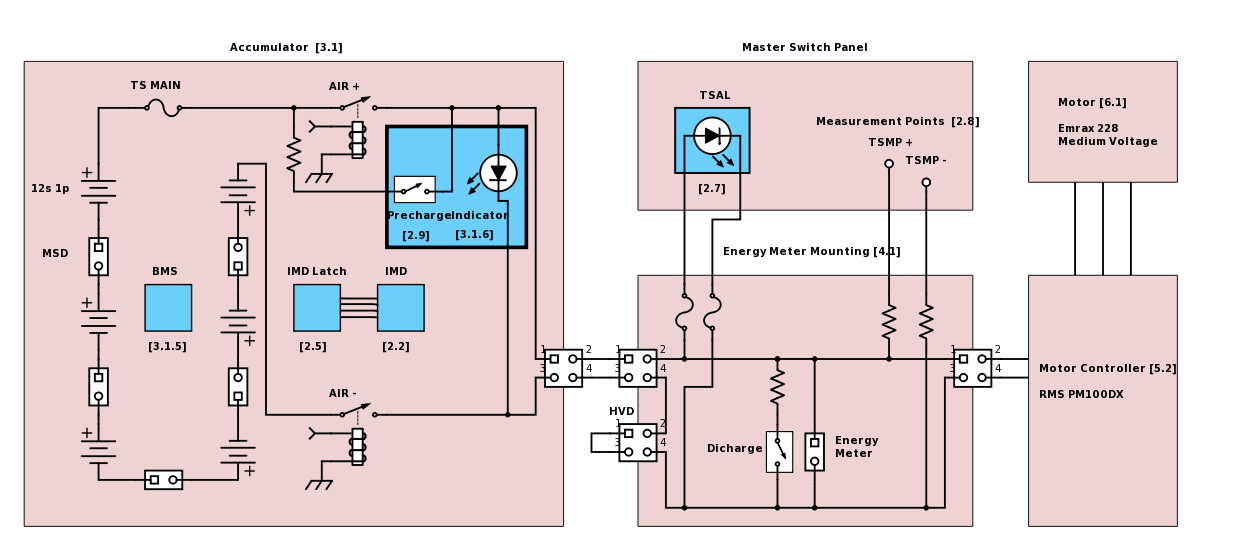
\includegraphics[width = 0.9 \textwidth]{TS-Block-Diagram.png}
  \caption{Block diagram of the enclosures of the Tractive System}
  \label{fig:TS_block_diagram}
  \end{figure}


\section{Electrical Systems}\label{electrical_systems}

\subsection{Shutdown Circuit}\label{shutdown_circuit}

\subsubsection{Description/ concept}
%Describe your concept of the shutdown circuit, the master switches, shut down buttons, brake over travel switch, etc.

The shutdown circuit directly controls the current that closes the AIRs. Since each switch/relay on the shutdown circuit is connected in series, that current must pass through every switch and safety check. If any device on the circuit is triggered by an unsafe condition, the current to the AIRs is cut off and the AIRs open, disconnecting the accumulator from the tractive system. Any capacitive load on the tractive system outside the accumulator is then discharged to ensure that all high voltage is contained inside the accumulator. 

	\begin{itemize}
		\item The GLV Master Switch (GLVMS) controls power to the entire low voltage system including the AIRs. As a result, high voltage cannot be present when the low voltage system is not active. The GLVMS has a lockout such that the vehicle can be safely worked on. 
		\item The Left E-Stop is a large red push-rotate button located at approximately the height of the driver's head on the left side of the vehicle. 
		\item The Right E-Stop is identical to the Left E-Stop located on the other side of the vehicle. 
		\item The Brake System Plausibility Device (BSPD) holds a normally open relay closed when it has not detected an implausibility. When it does detect an implausibility, it latches in a low state until the GLV system is power cycled. This shuts down the Tractive System in the event that the brake is pressed while the motors are being significantly driven.  
		\item The Brake Over Travel Switch (BOTS) is a push pull switch located behind the brake pedal. If the pedal over travels, the switch is pushed into an open state and stays that way until it is pulled back into the closed state. This shuts down the Tractive System in the event that brake pressure is lost. 
		\item The Dashboard E-stop functions the same as the other E-stops. It is located such that it can be easily pressed by the driver. 
		\item The Inertia Switch operates as a crash sensor that opens the shutdown circuit in the event that it detects an acceleration indicative of a collision. This ensures that the vehicle is electrically safe in an emergency situation. 
		\item The Battery Management System (BMS) monitors the condition of the accumulator. It holds a normally open relay closed while the lithium cells are operating within safe temperature and electrical conditions. 
		\item The Insulation Monitoring Device (IMD) detects any loss of isolation between the Tractive and GLV systems. It's output is held high while isolation is maintained. This holds a normally open relay closed through a latching circuit that prevents the IMD from re-closing the relay if the output goes low and then returns high. This latches the Tractive System in a shutdown state until the GLV system is power cycled. 
		\item The HVD interlock closes the shutdown circuit whenever the HVD is present. This automatically shuts down the Tractive System whenever the HVD is removed. 
		\item There is an interlock on the Tractive System connector on the accumulator which can be removed without tools. If the connector is removed, the Tractive System automatically shuts down. 
		\item The Tractive System Master Switch (TSMS) is the last switch in the shutdown circuit before the AIRs. It has a lockout such that the vehicle can be safely worked on. 
		\item Both the Pre-charge Relay and positive pole AIR have software controlled MOSFETs in series after them such that the timing of the pre-charge can be controlled by the sensing system.  
	\end{itemize}

	\begin{table}[H]
        \centering
        \begin{tabular}{|l|l|}
        \hline
            \textbf{Part} & \textbf{Function} \\ \hline
            GLV Main Switch (GLVMS) & Normally open, with lockout \\ \hline
            Shutdown buttons (SDB) (Left, right, cockpit) & Normally closed \\ \hline
            Brake System Plausibility Device (BSPD) & Normally Open \\ \hline
            Brake over travel switch (BOTS) & Push-pull normally closed button \\ \hline
            Inertia switch & Normally closed \\ \hline
            Battery Management System (AMS) & Normally open \\ \hline
            Insulation Monitoring Device (IMD) & Normally open \\ \hline
            Interlocks & Closed when TS connections are made \\ \hline
            Tractive System Main Switch (SMS) & Normally open, with lockout \\ \hline
        \end{tabular}
        \caption{List of switches in the shutdown circuit}
        \label{switchlist}
    \end{table}

\subsubsection{Wiring / additional circuitry} \label{sec:shutdown_wiring}

%TODO spec the breaker
	\Fref{fig:shutdown_circuit} shows the wiring of the shutdown circuit except the interlocks, which are detailed in section \ref{shutdown_system_interlocks}. The AIRs can only be closed and the tractive system energized when all of the elements of the shutdown circuit are closed. The shutdown circuit is expected to handle a maximum peak current of under 8A, so the wire gauge being used is 20AWG, protected by an appropriately-rated circuit breaker that is housed in the master switch panel. 


	\begin{sidewaysfigure}[p]
        \includegraphics[width= 1\textheight]{shutdown_circuit}
        \caption{Block Diagram of Shutdown Circuit}
        \label{fig:shutdown_circuit}
    \end{sidewaysfigure}

	\begin{table}[H]
        \centering
        \begin{tabular}{|l|l|}
        \hline
            Total Number of AIRs: & 2 \\ \hline
            Current per AIR & 3.9A peak while closing, 0.23 A average\\ \hline
            Additional parts consumption within the shutdown circuit: & 0.067 A (pre-charge and discharge relays)  \\ \hline
            Total current: & 7.867 A peak (everything closing simultaneously) \\ \hline
            Cross sectional area of the wiring used: & 0.52 mm$^2$ (20 AWG) \\ \hline
        \end{tabular}
        \caption{Wiring- Shutdown Circuit}
        \label{ShutdownCircuitTable}
    \end{table}

\subsubsection{Position in car}
%Provide CAD-renderings showing the relevant parts. Mark the parts in the renderings, if necessary.
The shutdown circuit passes through five major enclosures on the vehicle. It originates in the master switch panel, then passes through the BSPD in the bulkhead enclosure, then through the cockpit E-stop in the dashboard, and into the IMD and the BMS latches in the accumulator, finally going to the AIRs and out to the discharge circuit in the energy meter enclosure. It also passes through the side E-stop switches along the way. \newline

The shutdown circuit is wired between enclosures through waterproof TE Ampseal automotive connectors, is wrapped in abrasion-resistant mesh, and positively retained to chassis members with zip ties. Low voltage wiring is independently retained from high voltage wiring, and a minimum of 30mm separation is maintained. 


\subsection{IMD}\label{imd}
\subsubsection{Description (type, operation parameters)}%TODO

The IMD used will be a Bender A-ISOMETER IR155-3204. The output is normally high and only low if it detects an isolation fault. The output is then sent to the IMD latch board, where it is powers a SPST-NO relay which closes a switch in the shutdown circuit. The output of the IMD is also monitored directly by an ATmega on the AIR control board. \hl{The status of the IMD is also monitored by the BMS master, which sends messages to the dashboard over CAN to toggle the IMD light.} The IMD has a start up time of $\leq$ 2s. Further information on the IMD can be found in the appendix, section \ref{IMD_datasheet}.




%Describe the IMD used and use a table for the common operation parameters, like supply voltage, set point, etc. Also describe how the IMD indicator light is wired, etc.


\begin{center}
	\begin{table}[H]
		\begin{tabular}{|l|l|}
			\hline
			Supply voltage range: &  10..36VDC \\
			\hline
			Supply voltage: &  12VDC\\
			\hline
			Environmental temperature range: &  -40..105$^{\circ}$C \\
			\hline
			Selftest interval: &  Always at startup, then every 5 minutes \\
			\hline
			High voltage range: &  DC 0..1000V \\
			\hline
			Set response value: &  100k$\Omega$ \\
			\hline
			Max. operation current: &  150mA \\
			\hline
			Approximate time to shut down at 50\% of the response value:&  $\leq$ 40s \\
			\hline
		\end{tabular}
		\caption{Parameters of the IMD}
		\label{IMDParameters}
	\end{table}
\end{center}



\subsubsection{Wiring/cables/connectors/}
%Describe wiring, show schematics, describe connectors and cables used and show useful data regarding the wiring including wire gauge/temp/voltage rating and fuses protecting the wiring.
%TODO 

The  IMD uses the TYCO-MICRO MATE-N-LOK 1 x 2-1445088-8 connector and it's mate. \hlr{It connects to the IMD latch using 5-pin Molex LLC 1722861105 connectors. The signal is also sent to the BMS Master. The 18 AWG wire is more than sufficient for 150mA current draw of the IMD. The 18 AWG wire has a cross sectional area of 0.83mm$^2$, and is rated for at least 90\textdegree C, 300 V, and 16 amps. The HV wires to the IMD are protected by 3.15A fuses located on the pre-charge board. These fuses are identical to the fuses used to protect the TSAL, located in the energy meter enclosure documented in section {\ref{energy_meter_mounting}}. The datasheet can be found in section {\ref{appendix_energy_meter_mounting}}. The pre-charge board, seen to the left of the IMD in figure {\ref{fig:accumulator_top_view}}, is connected to TS+ and TS- (on the car side of the AIRs), as well as BAT+. It passes fused TS+ and TS- to the IMD. } 


\begin{figure} [!ht]
	\centering 
	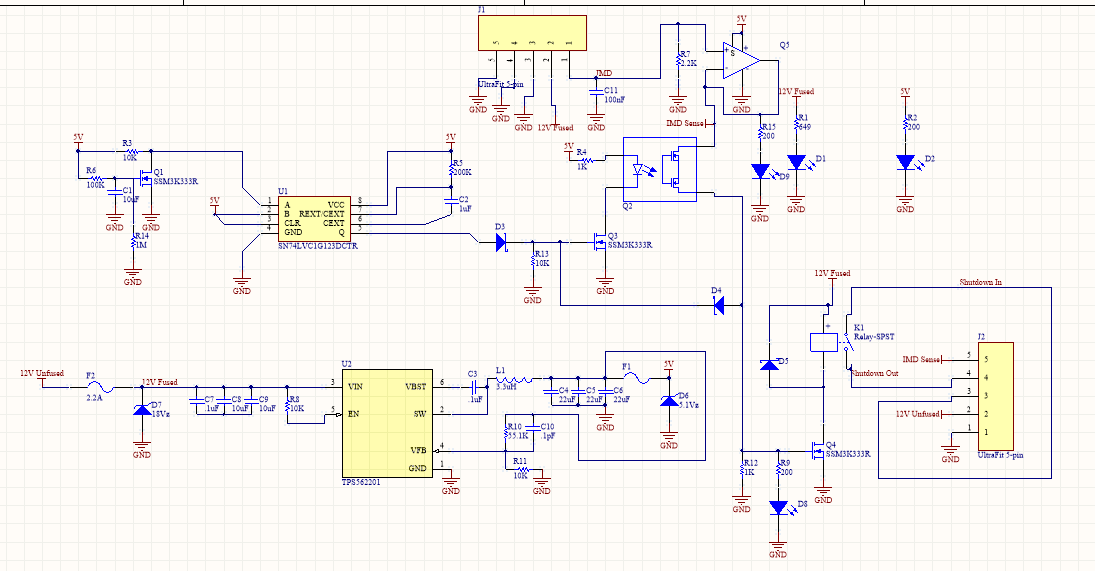
\includegraphics[width=1\textwidth]{IMD_Latch_Rev2_AltiumSchematic.PNG}
	\captionsetup{margin={0.3\textwidth,0.3\textwidth}}
	\caption{\hlr{The schematic for the IMD Latch.}}
	\label{fig:IMDLatch_Schematic}
\end{figure}

The IMD latch shown in \fref{fig:IMDLatch_Schematic} uses the signal from the IMD to close a relay in the shutdown circuit. In order for the shutdown relay to close a second relay needs to be closed. The second relay is initially powered by a one shot 4 second pulse from the GLV system. After the first four seconds the signal from the IMD is used to keep the secondary relay closed. If the IMD signal goes low the secondary relay will close. This opens the shutdown relay and makes it impossible for the IMD to close the shutdown relay again until the latch has been manually reset. The initial 4 second pulse is necessary to ensure that anomalous start up behavior from the IMD does not cause the secondary relay to open and force a manual reset.
%Describe wiring, show schematics, describe connectors and cables used and show useful data regarding the wiring including wire gauge/temp/voltage rating and fuses protecting the wiring.


\subsubsection*{2.2.3 Position in car}
%Position in car
%Provide CAD-renderings showing the relevant parts. Mark the parts in the rendering, if necessary.

The IMD will be located inside the accumulator, as shown in \fref{fig:accumulator_top_view}. \hl{It is located in the accumulator for continual monitoring of pack isolation while the accumulator is removed for charging.}

\begin{figure}[H]
    \centering 
    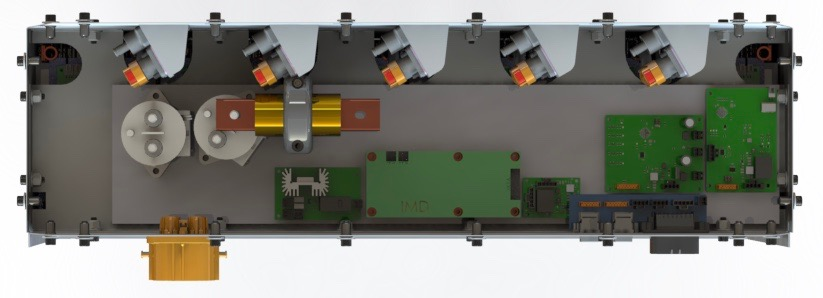
\includegraphics[width=1\textwidth]{Accum_top_view.jpg}
    \captionsetup{margin={0.3\textwidth,0.3\textwidth}}
    \caption{\hlr{View of the top of the accumulator}}
    \label{fig:accumulator_top_view}
\end{figure}


\subsection{Inertia Switch}\label{inertia_switch}
\subsubsection{Description (type, operation parameters)}
%Describe the Inertia Switch used and use a table for the common operation parameters, like supply voltage, temperature, etc.
The Sensata Resettable crash sensor (6-11g version) will trigger due to an impact that decelerates the vehicle between 6-11g.


	\begin{table}[H]
	    \centering
	    \begin{tabular}{|l|l|}
	    \hline
	    Inertia switch type & Sensata 6-11g crash sensor \\ \hline
	    Supply voltage range & 12 VDC \\ \hline
	    Supply voltage & 12VDC \\ \hline
	    \begin{tabular}[c]{@{}l@{}}Environmental temperature\\ range\end{tabular} & -10-120\degree C \\ \hline
	    Maximum operational current & \begin{tabular}[c]{@{}l@{}}20A for max. duration 30sec, \\ 10A max. continuous\end{tabular} \\ \hline
	    Trigger characteristics & \begin{tabular}[c]{@{}l@{}}Operate above 11g peak, 60ms duration\\ Not operate below 6g peak, 60ms duration\end{tabular} \\ \hline
	    \end{tabular}
	    \caption{Parameters of the Inertia Switch}
	    \label{InertiaTable}
	\end{table}

\subsubsection{Wiring/cables/connectors/}
            The Inertia switch will be wired to open the shutdown circuit in the case that there is a crash. The inertia switch is wired in-line with the shutdown circuit to be normally closed. Please see \fref{fig:shutdown_circuit} for the position of the inertia switch relative to the other shutdown system components.

\subsubsection{Position in car}
\hlr{The inertia switch will be located on the side of the dashboard enclosure. It is mounted upwards, so the top body panel will have to be temporarily removed to reset it,} as seen in \fref{fig:inertia_switch_mount}.

  \begin{figure}[H]
  \centering
  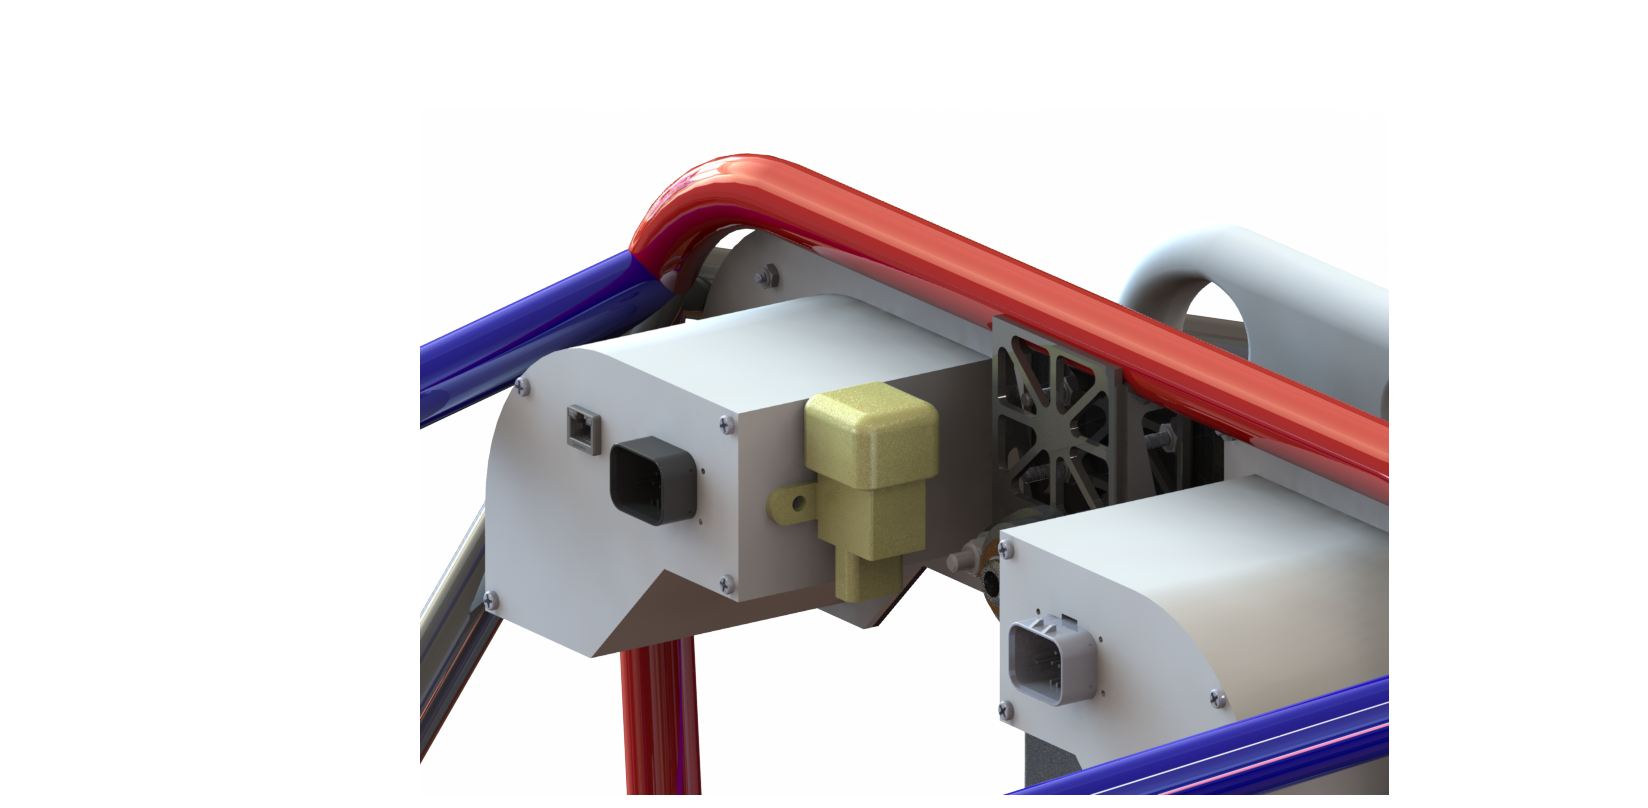
\includegraphics[width = 0.9 \textwidth]{ImpactSensor3-1-17}
  \caption{Positioning of the inertia switch alongside the dashboard enclosure}
  \label{fig:inertia_switch_mount}
  \end{figure}


\subsection{Brake Plausibility Device (BSPD)}\label{brake_plausibility_device}
\subsubsection{Description/additional circuitry}
%Describe how your electronic hardware brake plausibility system works (this is in addition to your ECU controlled brake plausibility software), provide tables with main operation parameters, and describe additional circuitry used to check or for an implausibility. Describe how the system reacts if an implausibility or error is detected.

The Brake System Plausibility Device (BSPD) is a custom circuit designed to open a relay in the shutdown circuit if the brakes are being pressed while there is positive-current being delivered to the motors for more than 0.5 seconds. The custom circuit takes in two digital signals, the brake signal and a boolean yes/no whether or not positive-current is being delivered to the motor. The positive-current will be sensed with our BMS using a hall-effect current sensor and a comparator which will output high when positive-current is being delivered to the motors. \\

\hl{The BMS uses a LEM HO 50-S hall effect current sensor. With our nominal pack voltage of 237.6V, it switches at 21A or 5kW to comply with EV5.6. As can be seen in the datasheet, which can be found in section {\ref{appendix_bspd}}, the sensor has a sensitivity of 16 mV/A. Figure {\ref{fig:bms_current_sense_schematic}} shows the circuit on the BMS, which amplifies the signal relative to the hall effect reference voltage with a gain of 2. Therefore, the threshold for 5kW of output power is at 672mV. This signal is compared to a voltage divider of a 100k resistor and a 14.3k resistor. With our VCC at 5V, this voltage divider outputs a value of 626mV, which sets the comparator to trigger high at a comfortable margin below the 5kW threshold.}\\

There are two main sections to the circuit: the timing section and the latching section. The timing section consists of a 555-timer in monostable mode which is configured to be powered from the output of an AND-gate which takes in both the brake signal and the positive-current signal. This 555-timer will output a high pulse if the AND gate outputs a high voltage for more than 0.5 seconds. \\

The latching section of the circuit is a simple SR-latch, which will hold the relay open when tripped by the timing section. \hl{The relay is held open until power is reset. Shortly after the circuit is powered, the 1G123 monostable multivibrator outputs a 1ms long pulse to set the latch, and close the shutdown circuit.} \\

The schematic can be seen in \fref{fig:bspd_schematic}. \\

	\begin{table}[H]
	    \centering
	    \begin{tabular}{|l|l|}
	    \hline
	    Brake sensor used: & Pegasus Brake Light switch, part 3601 \\ \hline
	    Torque encoder used: &  \hl{Magni-Tec} MHR5621\\ \hline
	    Supply voltages: & 5V \\ \hline
	    Maximum supply currents: & 15 mA\\ \hline
	    Operating temperature: & -55 to 150\degree C \\ \hline
	    Output used to control AIRs: & Opens a relay \\ \hline
	    \end{tabular}
	    \caption{Torque Encoder Data}
	    \label{TorqueEncoder1}
	\end{table}


\subsubsection{Wiring}
%Describe the wiring, show schematics including the circuit board, show data regarding the cables and connectors used.  If not detailed in section 2.1, be sure to show how the device open the shutdown circuit.

The output of the BSPD circuit will low-side drive a relay in series with the shutdown circuit. This board has not been fully designed, but it will utilize components common across other circuits.

  \begin{figure}[H]
        \centering
        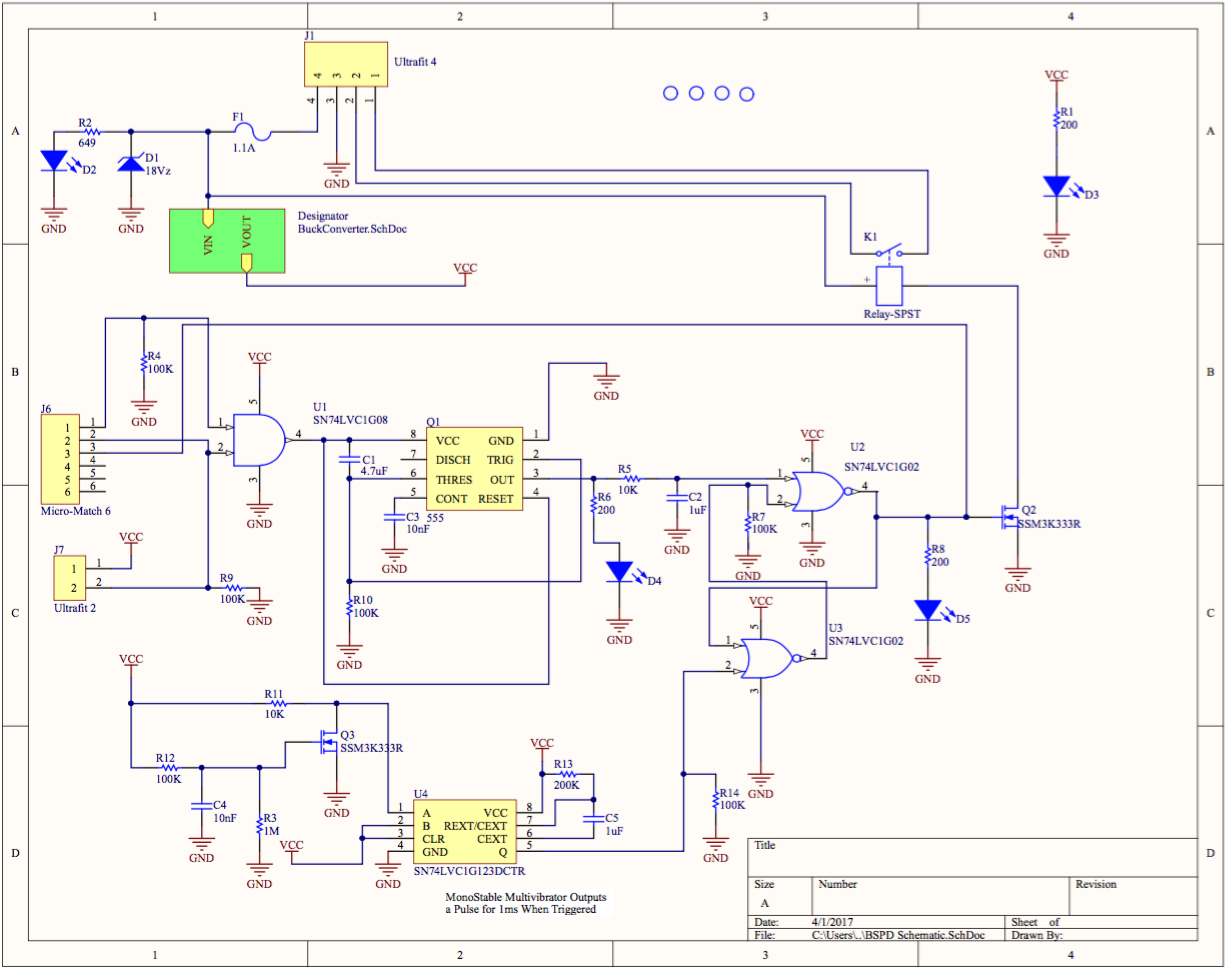
\includegraphics[width=\textwidth]{bspd_schematic_rev2.png}
        \caption{\hl{Schematic for BSPD circuit}}
        \label{fig:bspd_schematic}
  \end{figure}

  \begin{figure}[H]
        \centering
        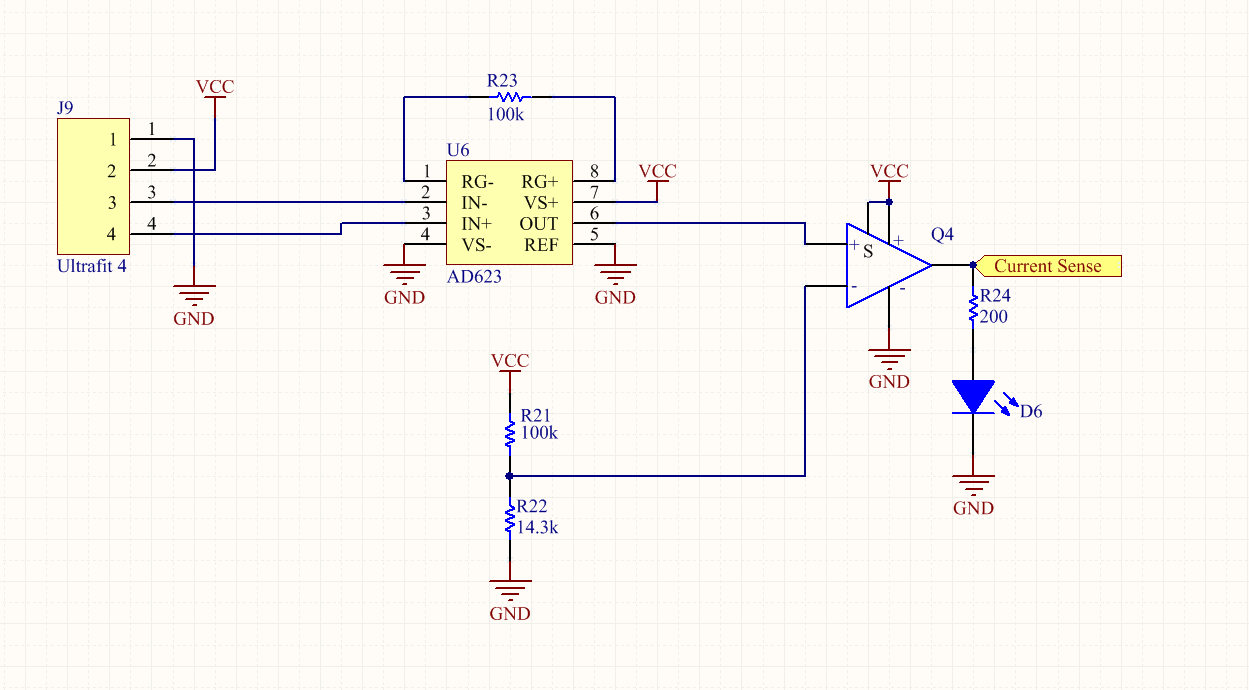
\includegraphics[width=\textwidth]{BMS_current_sense_schematic.png}
        \caption{\hl{Schematic for BMS current sensing circuit}}
        \label{fig:bms_current_sense_schematic}
  \end{figure}

\subsubsection{Position in car/mechanical fastening/mechanical connection}
%Provide CAD-renderings showing all relevant parts and discuss the mechanical connection of the sensors to the pedal assembly. Mark the parts in the rendering, if necessary.

This board is located in the bulkhead enclosure at the front of the car.

\subsection{Reset / Latching for IMD and BMS}\label{reset_latching_for_imd_and_bms}
\subsubsection{Description/circuitry}
%Describe the concept and circuitry of the latching/reset system for a tripped IMD or BMS.  Describe the method for resetting the IMD and BMS.

Resetting the IMD latch, which is shown in \fref{fig:IMDLatch_Schematic} , requires restarting the GLV system. Restarting the GLV system will cause the IMD latch to send a pulse. If the output of the IMD is high because there is no ground fault, the pulse from the GLV activation will close the secondary relay, which allows the signal from the IMD to close the shutdown circuit.\\

\hl{The BMS master controls a normally open relay on the shutdown circuit. In the case that the BMS detects a fault in cell temperature or voltage that requires a vehicle shutdown, the ATmega16m1 on the board opens the relay, and does not close the relay until it power cycled. Essentially, the BMS master is programmed to close its relay only once per power cycle. The master BMS will also serve as a CAN network monitor, and if another node in the vehicle detects a fault condition that requires vehicle shutdown that is not rules-required to be analog circuity, that node will send a shutdown message to the master BMS that will open the shutdown circuit. }

\subsubsection{Wiring/cables/connectors}
%TODO
%Describe wiring, show schematics, describe connectors and cables used and show useful data regarding the wiring.  If not detailed in section 2.1, be sure to show how the device opens the shutdown circuit.
The IMD latch will be connected to the accumulator interface board board via a \hlr{5-pin Molex LLC Ultrafit 1722861105 with 18 AWG wire, and the IMD connector using another 5-pin Molex LLC Ultrafit of the same type. The 18 AWG wire has a cross sectional area of .83mm$^2$, and is rated for at least 90\textdegree C, 300 V, and 16 amps.} This provides a considerable safety margin. The ribbon cable carries signals from the IMD. 18 AWG wire is used for the shutdown circuit and to supply power and ground to the IMD latch. The 18 AWG wire has a cross sectional area of .83mm$^2$, and is rated for 16 amps for chassis wiring and 2.3 amps for power transmission. The 18 wire will be rated for at least 90\textdegree C and 300~V, as required by the rules for wiring in the accumulator (see EV3.3.8 and EV4.5.4).\\


Similarly to the IMD latch, the BMS will be housed in the accumulator, and thus all of the shutdown circuit connections to and from it will be made with 18AWG wire rated to over 300V and 90\textdegree C in order to handle the maximum of \hl{5A} inrush current to the AIRs and maintain compliance with accumulator wiring regulations. PCB traces will also be appropriately sized to handle \hl{5A} peak current. 
% connects to IMD through either accumulator interface or AIR control.


\subsubsection{Position in car}
%Provide CAD-renderings showing the relevant parts. Mark the parts in the rendering, if necessary.
The IMD, IMD latch, and the BMS are in the accumulator, as shown in \fref{fig:accumulator_hero}. BMS is positioned there for ease of access to the battery, and the IMD latch is positioned there in order to be close to the IMD, which is located in the accumulator for continual monitoring of pack isolation while the accumulator is removed for charging. 

\subsection{Shutdown System Interlocks}\label{shutdown_system_interlocks}
\subsubsection{Description/circuitry}
%Describe the concept and circuitry of the Shutdown System Interlocks.
%Note: Interlocks are circuits used to open the shutdown circuit if a connector is disconnected or enclosure is opened.  This is not the entire shutdown circuit.
The vehicle's tractive system connectors are all lever action locking connectors from the TE Connectivity HVP 800 series. Their arrangement in the tractive system can be seen in \fref{fig:HV_connector_diagram}. These connectors can be removed without tools. In compliance with EV 3.3.6, \hl{the accumulator connector and HVD contain an interlock that opens the shutdown circuit when they are not installed.} 

  \begin{figure}[H]
        \centering
        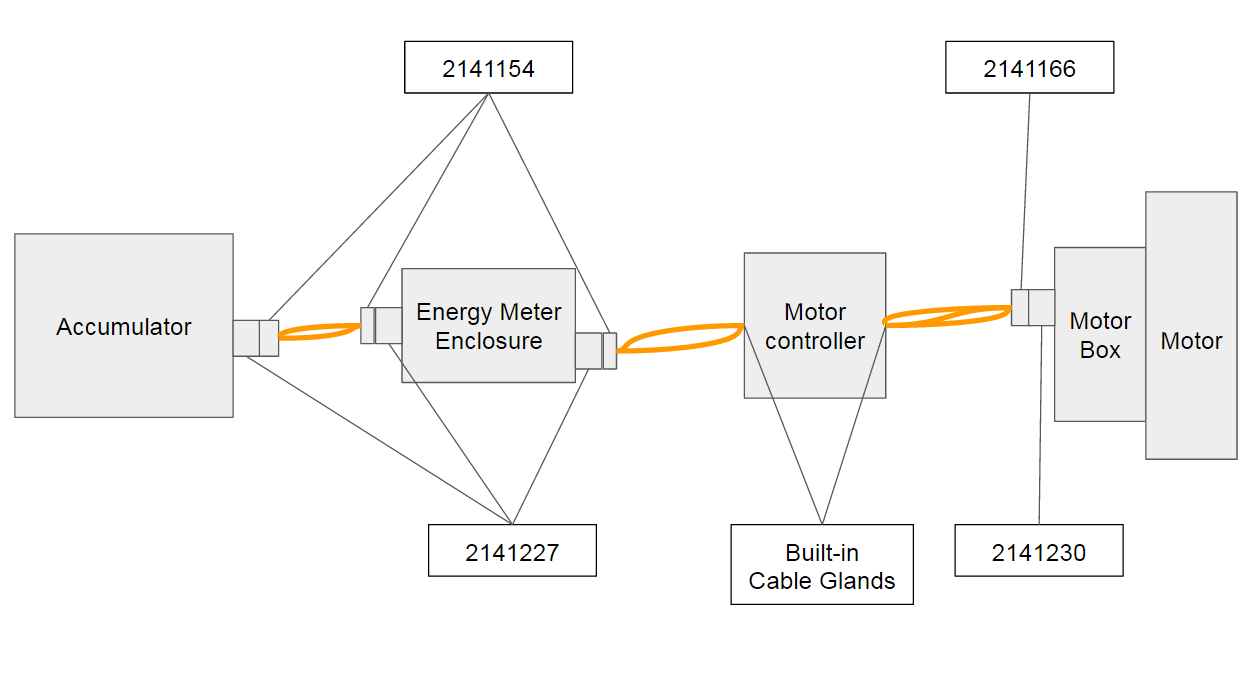
\includegraphics[width=.75\textwidth]{HV_connector_diagram.png}
        \caption{Diagram of HV connectors in the tractive system. They are labelled with TE Connectivity part numbers.}
        \label{fig:HV_connector_diagram}
  \end{figure}

In order to close the shutdown circuit during charging when the accumulator is removed from the vehicle, a connection must be made that overrides the interlocks in the HV connectors that remain with the vehicle. Our solution is a shunt in the LV charging connector that bypasses the circuit that normally connects \hl{HVD interlock}. The main accumulator connector interlock is still required to close the shutdown circuit, so EV 3.3.6 compliance is maintained. A schematic of this interlock circuitry can be seen in \fref{fig:HV_connector_schematic}.

\begin{figure}[H]
\centering
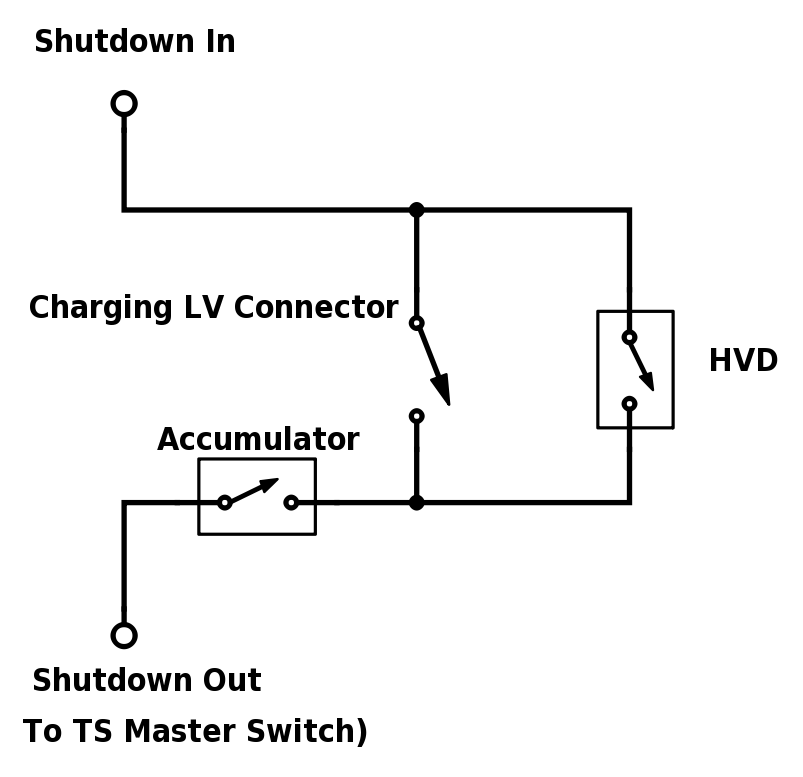
\includegraphics[width = .75\textwidth]{HV-connector-schematic.png}
\caption{Schematic of the HV interlocks in the vehicle. Note the LV connector that allows the shutdown circuit to close the AIRs when the vehicle is charging.}
\label{fig:HV_connector_schematic}
\end{figure}

\subsubsection{Wiring/cables/connectors}
%Describe wiring, show schematics, describe connectors and cables used and show useful data regarding the wiring.
The shutdown circuit interlock wires will be 20 or 22 AWG and rated to over 300V and 90\textdegree C and are protected by the main shutdown circuit breaker as in \fref{sec:shutdown_wiring}. 

\subsubsection{Position in car}
\hl{The accumulator connector is panel-mounted to the accumulator housing. The HVD is mounted on the energy meter enclosure, and is clearly visible from the rear of the vehicle.} See the render of the rear of the car in \fref{fig:rear_of_car}.

\begin{figure}[H]
\centering
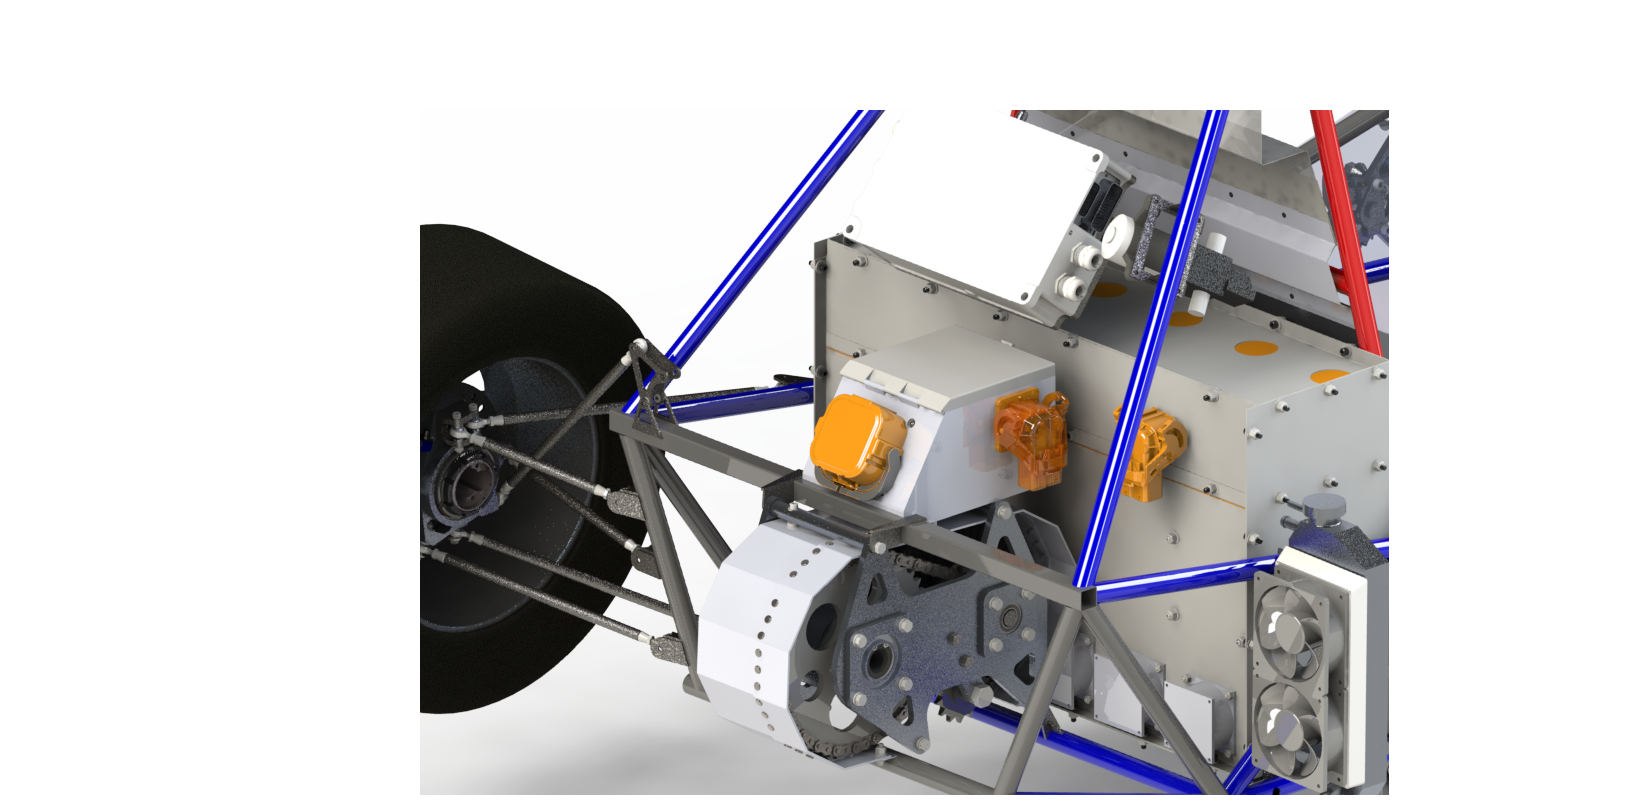
\includegraphics[width = .75\textwidth]{EnergyMeterBackISO}
\caption{Render of the rear of the vehicle showing location of HV connectors. \hlr{Connectors are highlighted in orange.} }
\label{fig:rear_of_car}
\end{figure}

\subsection{Tractive system active light}\label{tractive_system_active_light}
\subsubsection{Description/circuitry}
%Describe the tractive system active light and additional circuitry.
The TSAL illuminates when the tractive system is active, which is defined as the tractive system voltage being over 60V.

	\begin{table}[H]
	    \centering
	    \begin{tabular}{|l|l|}
	    \hline
	    Supply voltage: & 12V \\ \hline
	    Max. operational current: &  \hl{1.2A}\\ \hline
	    Lamp type: & LEDs \\ \hline
	    Power consumption: & \hl{14.4W (max)}\\ \hline
	    Brightness: & Unknown\\ \hline
	    Frequency: & 2 Hz \\ \hline
	    Size (length x height x width): & 41x41x32 mm \\ \hline
	    \end{tabular}
	    \caption{Parameters of the TSAL}
	    \label{TSALparameters}
	\end{table}
	
See the appendix \hyperlink{TSALdatasheet}{here} for a link to the TSAL Datasheet.

\subsubsection{Wiring/cables/connectors}
%Describe wiring, show schematics, describe connectors and cables used and show useful data regarding the wiring.  Include gauge, voltage and temperature rating of wiring used and any fuses or other overcurrent protection used.
\hl{The circuitry designed has a TS-controlled digital isolator whose power is supplied by the TS through two linear voltage regulators. When the TS is over 60V, a voltage divider with resistors of 30.1K and 1.91K causes the digital isolator to go logic high which allows the down regulated GLV to switch on the MOSFET allowing current to flow through the TSAL low side drive.} The frequency of the TSAL will be controlled by built in settings to flash at 2Hz. See \fref{fig:TSALcircuit} for a schematic diagram of the TSAL circuit.

\begin{figure}[H]
\centering
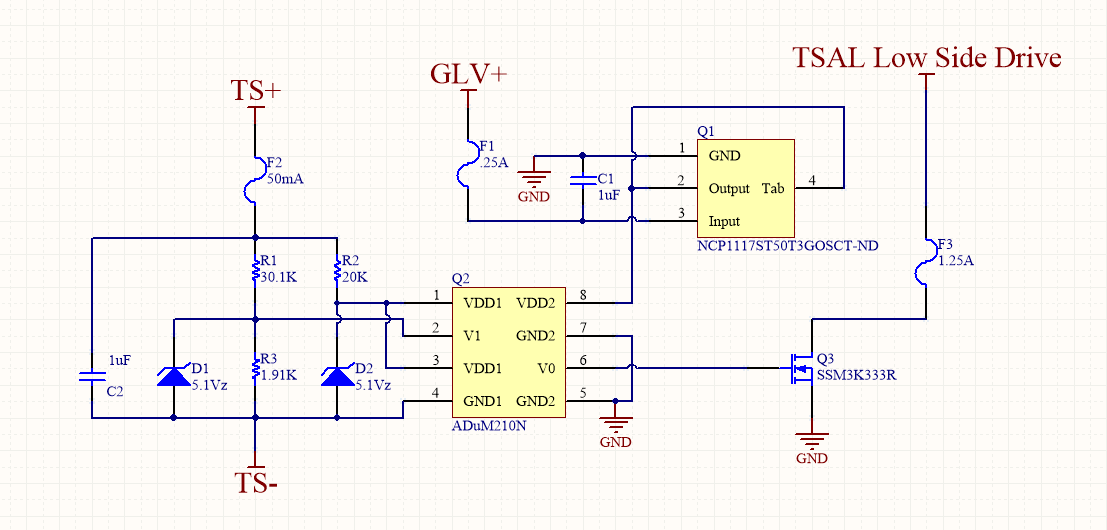
\includegraphics[scale=.7]{TSAL.png}
\caption{Schematic for the TSAL}
\label{fig:TSALcircuit}
\end{figure}

\hl{Per EV4.1.7, the HV and LV sides of the TSAL board are separated by at least 12.7 mm (1/2 in). See} \fref{fig:TSALspacing} \hl{for an image of the PCB layout.}

\begin{figure}[H]
\centering
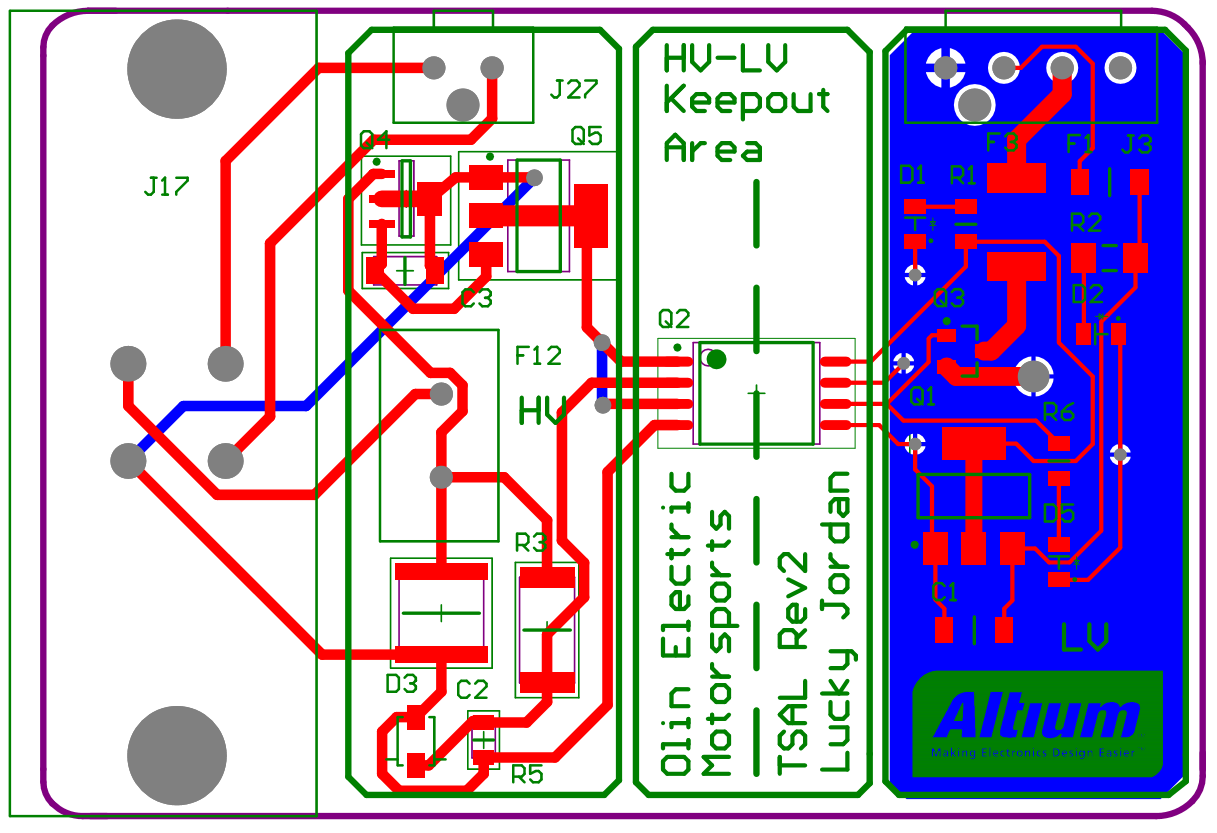
\includegraphics[scale=.7]{TSALspacing.png}
\caption{\hl{Spacing for the TSAL}}
\label{fig:TSALspacing}
\end{figure}

All connections made by wires will be 20 AWG rated for 600V, 125°C and 7A, while all PCB traces will be a minimum of 12 mil, but nominally 20 mil in width. The TS voltage will be fused to \hl{50mA}. The GLV voltage will be fused to \hl{.25A on the supply line for the digital isolator and 1.25A on the power line for the TSAL with traces of at least 60 mil}, able to handle \hl{1.5A} of current due to the \hl{1.2A} max current draw of the TSAL.

\hl{As seen in figure {\ref{fig:TS_block_diagram}}, the HV fuses for the TSAL are located in the energy meter enclosure, datasheet located in section {\ref{appendix_energy_meter_mounting}}. The HV wires from the energy meter enclosure to the master switch panel enclosure are shielded and covered in orange cable wrap, datasheet located in section {\ref{sec:appendix_TSAL}}}. 

\subsubsection{Position in car}
%Provide CAD-renderings showing the relevant parts. Mark the parts in the rendering, if necessary.
The TSAL will be mounted to the underside of the highest point of the main roll hoop, per EV 4.12.3 and 4.12.4 using a \hl{welded mount}. The PCB will be located in the master switch panel enclosure.

\begin{figure}[H]
\centering
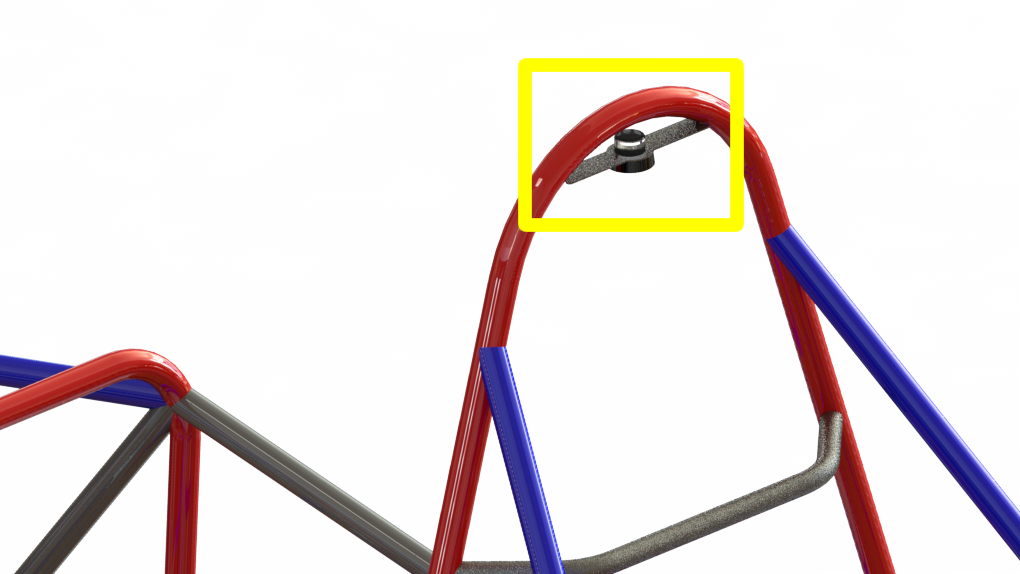
\includegraphics[scale=1]{TSAL_mounting.png}
\caption{CAD rendering of TSAL position under apex of main roll hoop}
\end{figure}

\subsection{Measurement points}\label{measurement_points}
\subsubsection{Description}
%Describe the housing used and how it can be accessed, etc.  Describe how the measurement points protected/covered when not in use and how the electrical connections on the back of the measurement points are protected when the measurement points are being used.
The TSMPs and GLVS ground measurement points are located on the master switch panel on the side of the vehicle, which also houses the TSAL circuitry in section \ref{tractive_system_active_light}. They will be a set of three clearly labeled and easily accessible shrouded banana jack connectors with hinged panel-mount covers to prevent any unintentional contact. These are visible in \fref{fig:master_switch_panel}. The measurement points provide a means for safe measurement of the tractive system potential , a secondary manual method for detecting isolation faults, and a reference point for system grounding  measurements. 


\subsubsection{Wiring, connectors, cables}
%Describe wiring, show schematics, and describe connectors and cables used and show useful data regarding the wiring.  Include details on the protection resistor including resistance, voltage and power rating.

\begin{figure}[H]
\centering
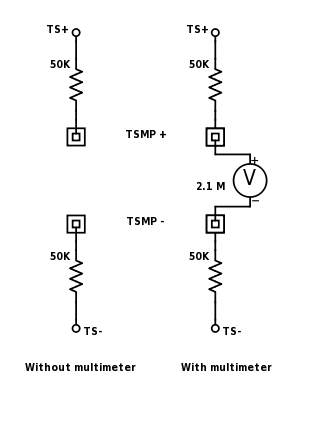
\includegraphics[scale=0.5]{TSMP-Schematic.png}
\caption{Schematic of TSMP wiring, illustrating the circuit with and without the multimeter, showing the protection resistors and the approximate expected resistance of the multimeter.}
\label{fig:TSMP_schematic}
\end{figure}

There are \hl{four} measurement points: HV+, HV-, \hl{GLVS+}, and GLVS chassis ground. The HV TSMP connections will protected with \hl{10k$\Omega$} current-limiting resistors. These resistors limit the maximum fault current (a short circuit between the measurement points) in accordance with EV4.4.6. 

\begin{align*}
V = I * R \\
300V = I * 20,000\Omega \\
I = 0.015A
\end{align*}

\begin{align*}
P = I * V \\
P = 0.015A * 300V \\
P = 4.5W
\end{align*}

According to the above calculations, the resistors will have to be rated to at least \hl{5W} and 300V. We will be using \hl{Vishay PAC500001002FAC000 10k 5W} resistors. The datasheets for the resistors, the connectors, and an example multimeter can be found in \fref{sec:appendix_TSMP}.

The TSMPs are protected with current-limiting resistors because protecting the wires with fuses introduces the failure mode in which one of the fuses has blown, and a measurement across the TSMPs shows an open circuit even though the tractive system is still energized. 

In case of gross operator error that results in connecting a multimeter from a TS measurement point to the GLVS ground measurement point, the IMD will detect a loss of isolation and open the shutdown circuit. 

\hl{As seen in figure {\ref{fig:TS_block_diagram}}, the current limiting resistors are located in the energy meter enclosure. The HV wires from the energy meter enclosure to the master switch panel enclosure are shielded and covered in orange cable wrap, datasheet located in section {\ref{sec:appendix_TSAL}}}.

\subsubsection{Position in car}
%Provide CAD-renderings showing the relevant parts. Mark the parts in the rendering, if necessary.
The TSMPs will be located in the master switch panel enclosure shown in \fref{fig:master_switch_panel} along with TSAL circuitry. The housing will be made of non-conductive material, and proper spacing between TS measurement point wiring and any part of the GLVS of 30mm through air will be maintained in accordance with EV 4.1.5.

\begin{figure}[H]
\centering
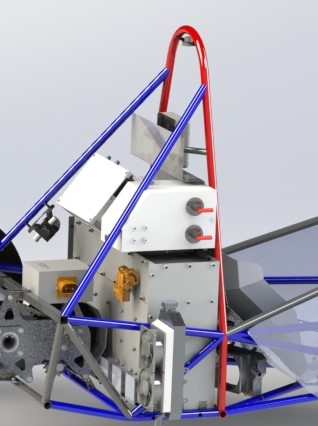
\includegraphics[scale=1]{MSP_Box_Angle}
\caption{CAD rendering of the master switch panel showing TS and GLVS master switches, and TS and GLVS ground measurement points. \hl{This current render has the enclosure protruding from the chassis envelope, but the enclosures team is currently redesigning the face of the master switch panel to be flush with the chassis members.}}
\label{fig:master_switch_panel}
\end{figure}

 
\subsection{Pre-Charge circuitry}\label{pre_charge_circuitry}
\subsubsection{Description}
%Describe your concept of the pre-charge circuitry.

In order to prevent inrush current that could damage the motor controller or AIRs, and to comply with EV4.11.1, our pre-charge circuit slowly charges the capacitive load of the motor controller through a power limiting resistor before closing the TS+ AIR. When the shutdown circuit closes, the TS- AIR is immediately closed, but the software controlled MOSFETs seen in \fref{fig:precharge_schem} will prevent the pre-charge relay and TS+ AIR from closing. After a short delay, the pre-charge relay is allowed to close. This delay is included to allow detection of a welded pre-charge relay. The motor controller tracks its pre-charge state, and signals over the CAN network to allow the TS+ AIR to close when pre-charge is complete. 

\subsubsection{Wiring, cables, current calculations, connectors}
%Describe wiring, show schematics, describe connectors and cables used and show useful data regarding the wiring.
%Give a plot “Percentage of Maximum Voltage” vs. time
%Give a plot Current vs. time
%For each plot, give the basic formula describing the plots

\begin{figure}[H]
    \centering
    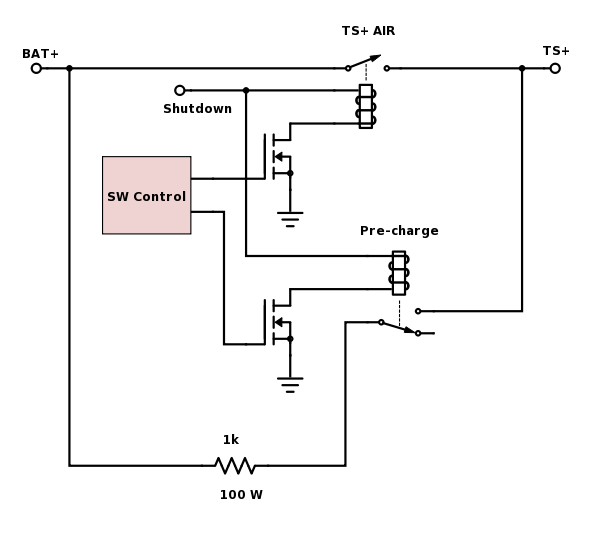
\includegraphics[width = 0.7 \textwidth]{precharge_schem}
    \caption{Schematic of the pre-charge circuit. Although the TS+ AIR and pre-charge relay are software controlled, the circuit is designed such that they cannot close if the shutdown circuit is open.}
    \label{fig:precharge_schem}
\end{figure}

\begin{figure}[H]
    \centering
    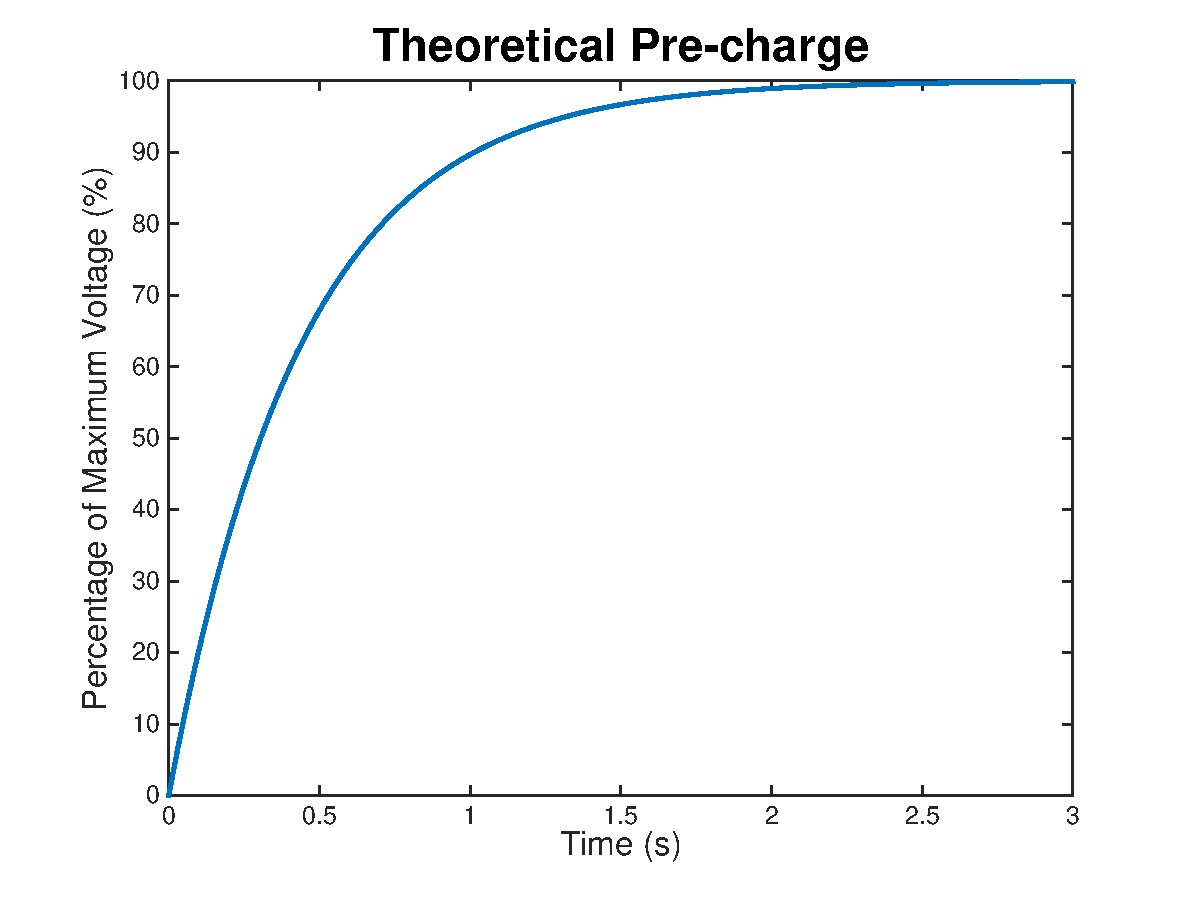
\includegraphics[width = 0.8 \textwidth]{precharge_voltage}
    \caption{Theoretical pre-charge of the 440$\mu$F motor controller capacitance using a 1$k\Omega$ resistor. This plot was created using the equation, $V(t) = V_{BAT}(1 - e^{-t/RC})$ where $V_{BAT}$ is our maximum pack voltage of just under 300VDC. Our motor controller is expecting an approximately 95\% pre-charge within 3 seconds, so this circuit covers the needs of our motor controller and is in compliance with EV4.11.1 }
    \label{fig:precharge_voltage}
\end{figure}

\begin{figure}[H]
    \centering
    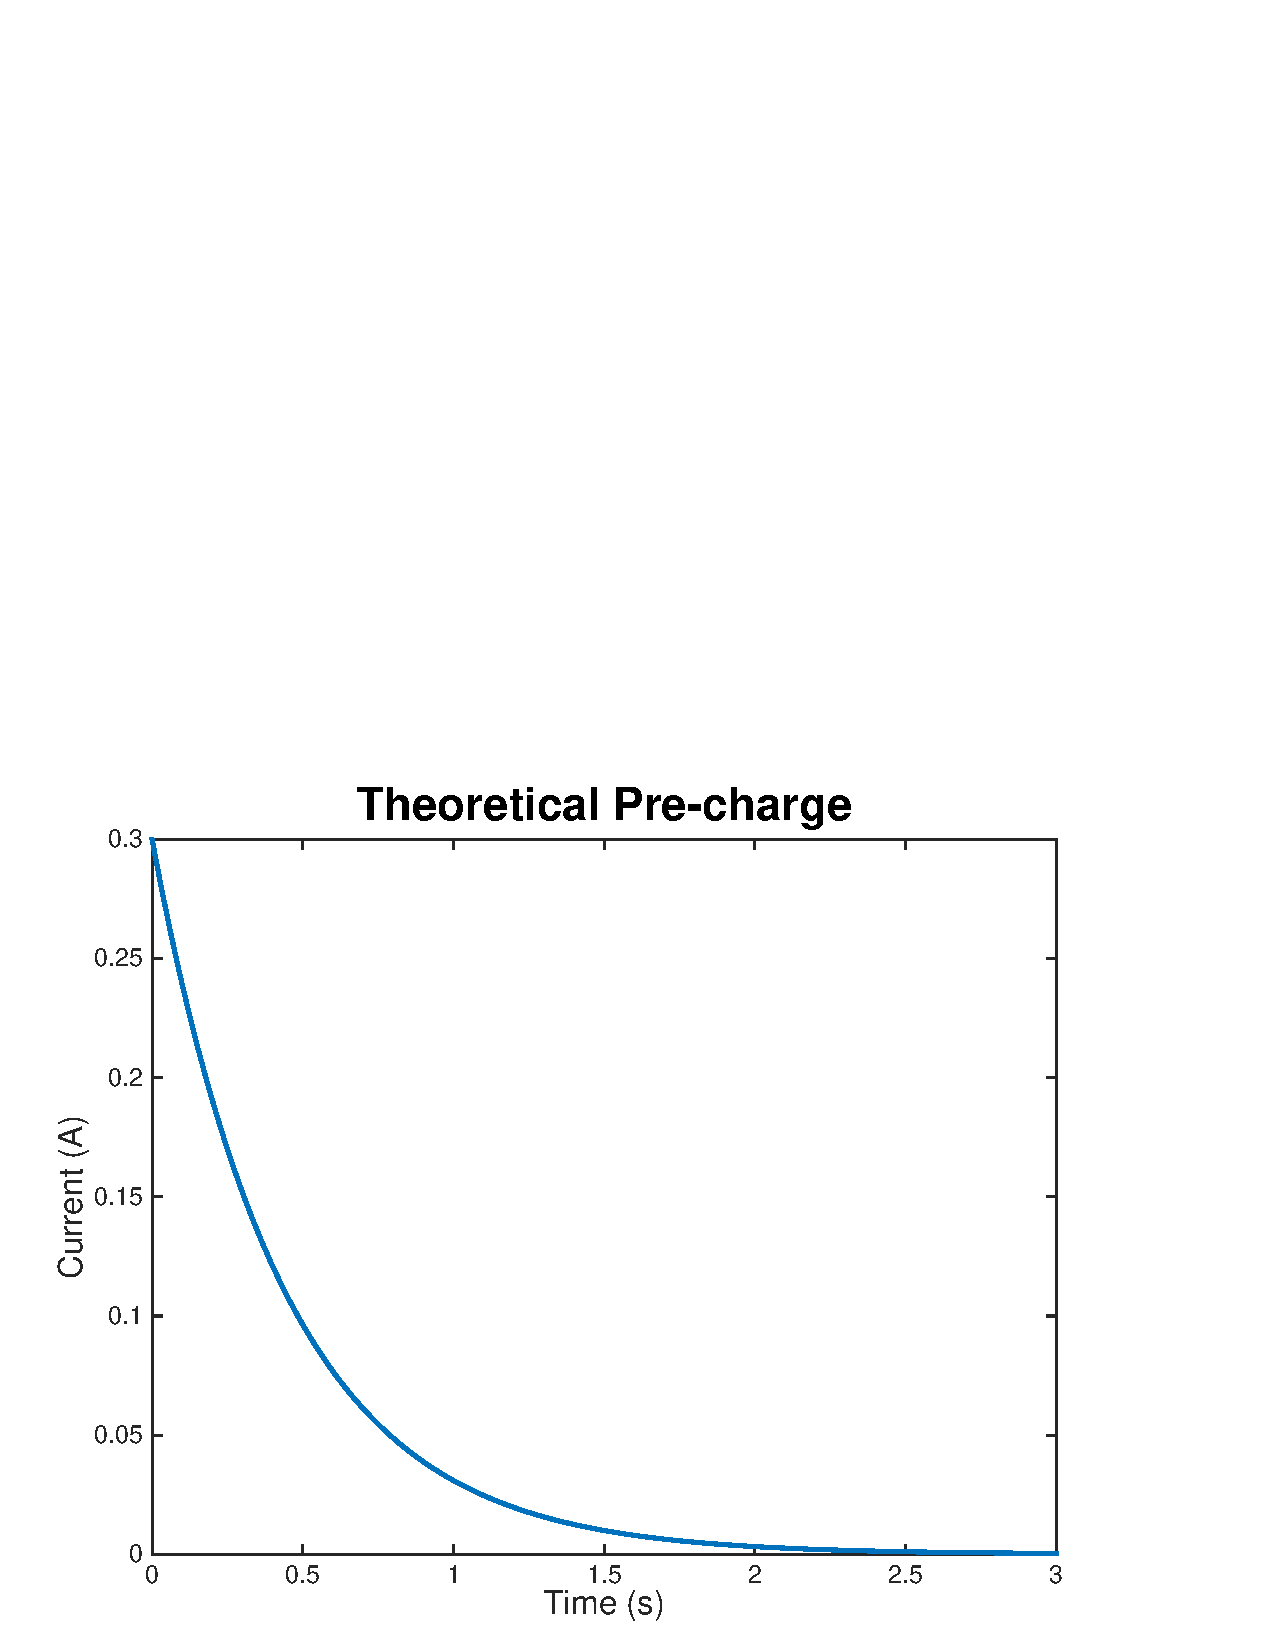
\includegraphics[width = 0.8 \textwidth]{precharge_current}
    \caption{The current of the theoretical pre-charge from \fref{fig:precharge_voltage}. This plot was created using the equation $I(t) = \frac{V(t)}{R}$ where $V(t)$ is the voltage across the pre-charge resistor found by the equation $V(t) = V_{BAT} * e^{-t/RC}$ }
    \label{fig:precharge_current}
\end{figure}

    \begin{table}[H]
	    \centering
	    \begin{tabular}{|l|l|}
	    \hline
	    Resistor type & Riedon PF2470 Power Film Resistor \\ \hline
	    Resistance & 1 $k\Omega$ \\ \hline
	    Continuous power rating & 100 W \\ \hline
	    Overload power rating & 140 W \\ \hline
	    Voltage rating & 700 V \\ \hline
	    Cross-sectional area of wire used & 0.83mm$^2$ (18 AWG)\\ \hline
	    \end{tabular}
	    \caption{General data of pre-charge resistor. \hl{See the datasheet in appendix section }\ref{appendix_precharge}.}
	    \label{prechargeresistor}
	\end{table}

	\begin{table}[H]
	    \centering
	    \begin{tabular}{|l|l|}
	    \hline
	    Relay type & Omron G2RL-1-E DC12 \\ \hline
	    Contact arrangement & SPDT \\ \hline
	    Continuous DC current & 16A \\ \hline
	    Voltage rating & 300VDC \\ \hline
	    Cross-sectional area of wire used & 0.83mm$^2$ (18 AWG) \\ \hline
	    \end{tabular}
	    \caption{General data of the pre-charge relay \hl{See the datasheet in appendix section }\ref{appendix_precharge}.}
	    \label{PCrelay}
	\end{table}

\subsubsection{Position in car}
%Provide CAD-renderings showing all relevant parts. Mark the parts in the rendering, if necessary.
The pre-charge circuit will be located within the accumulator. \hlr{The pre-charge circuitry will be located on the AIR control PCB seen in figure {\ref{fig:accumulator_top_view_2}} (the PCB with the heat sink) in the top section of the accumulator, as described in section {\ref{accumulator_mechanical_configuration}}.}

\begin{figure}[H]
    \centering 
    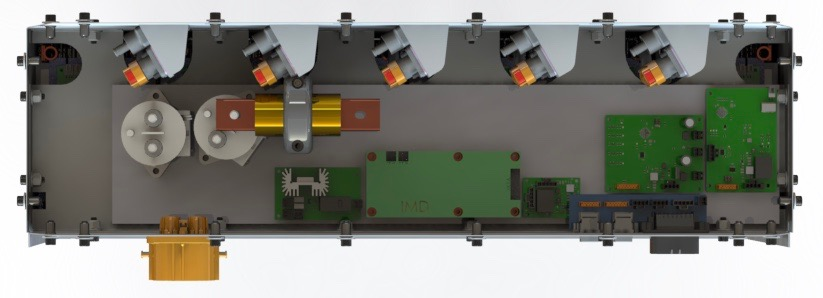
\includegraphics[width=1\textwidth]{Accum_top_view.jpg}
    \captionsetup{margin={0.3\textwidth,0.3\textwidth}}
    \caption{\hlr{View of the top of the accumulator}}
    \label{fig:accumulator_top_view_2}
\end{figure}

\subsection{Discharge circuitry}\label{discharge_circuitry}
\subsubsection{Description}
%Describe your concept of the discharge circuitry.
When the car is shut down, and the AIRs have disconnected the accumulator from the rest of the tractive system, there is still energy stored in the capacitive load of tractive system components like the motor controller that could be harmful to the driver, team members, or first responders. The discharge circuit dissipates the energy found on the vehicle side of the tractive system after a shutdown. The circuit is designed to operate even if the vehicle looses all power. When the shutdown circuit is opened, the normally closed discharge relay connects a power resistor across the two poles of the tractive system.  

\subsubsection{Wiring, cables, current calculations, connectors}
%Describe wiring, show schematics, describe connectors and cables used and show useful data regarding the wiring.
%Give a plot “Voltage” vs. time
%Give the formula describing this behavior
%Give a plot “Discharge current” vs. time
%Give the formula describing your plot

Since the power resistor limits the current on the discharge circuit, a fuse is not needed to protect the wiring. It is also dangerous for the discharge circuit to not operate if a fuse were to blow. 

\begin{figure}[H]
    \centering
    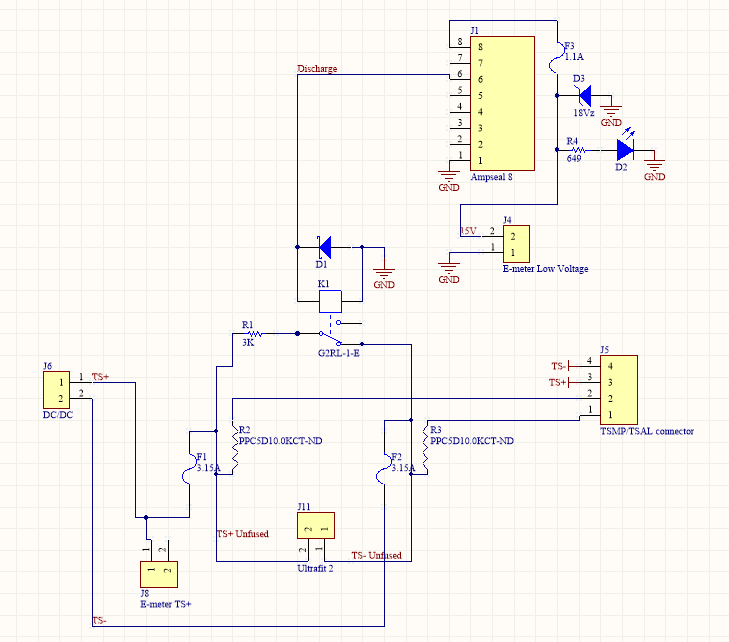
\includegraphics[width = 0.7 \textwidth]{Discharge.png}
    \caption{Schematic of the discharge system\hlr{. The wiring for the TSMPs, TSAL power, and E-meter connections are also visible.}}
    \label{discharge_schem}
\end{figure}

\begin{figure}[H]
    \centering
    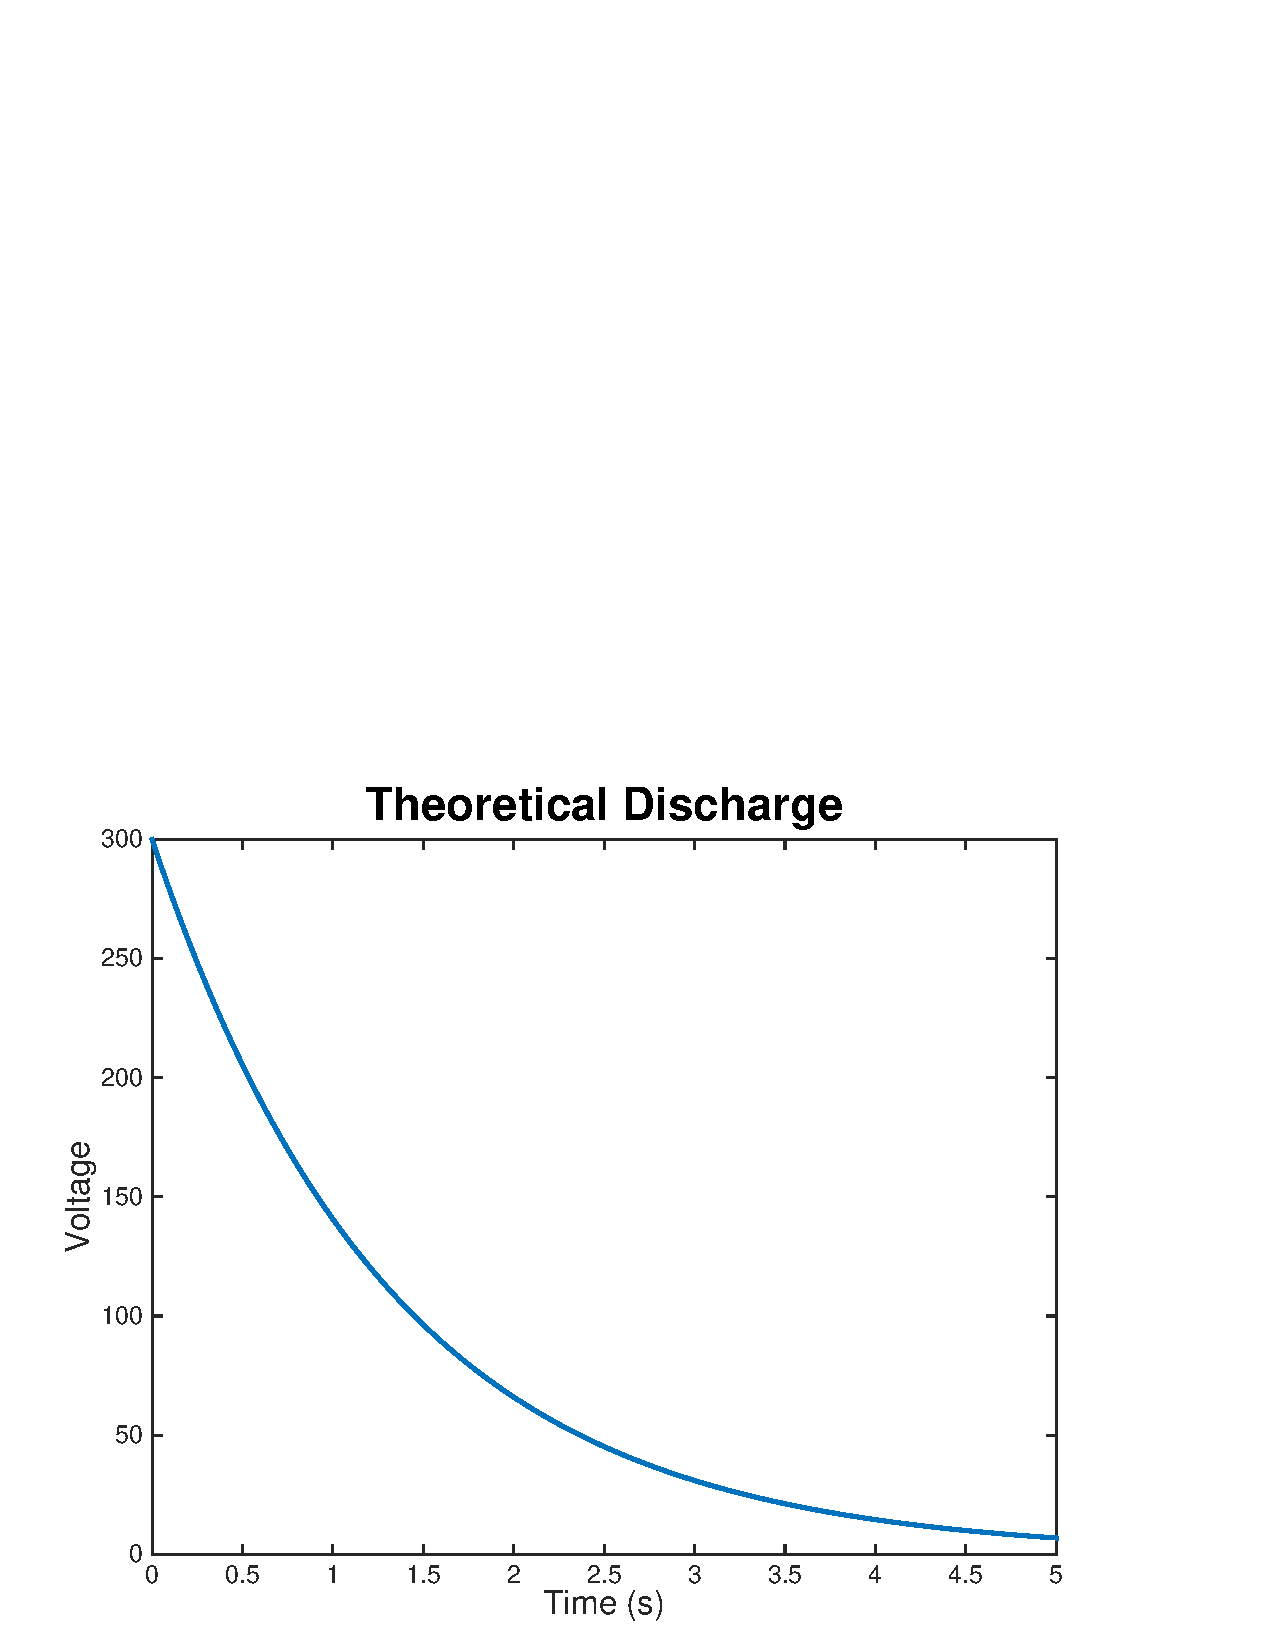
\includegraphics[width = 0.7 \textwidth]{discharge_voltage}
    \caption{Theoretical discharge of the 440 $\mu F$ capacitive load of the motor controller across the 3 k$\Omega$ resistor. This was calculated using the equation $V(t) = V_{0} * e^{-t/RC}$.}
    \label{fig:discharge_voltage}
\end{figure}

\begin{figure}[H]
    \centering
    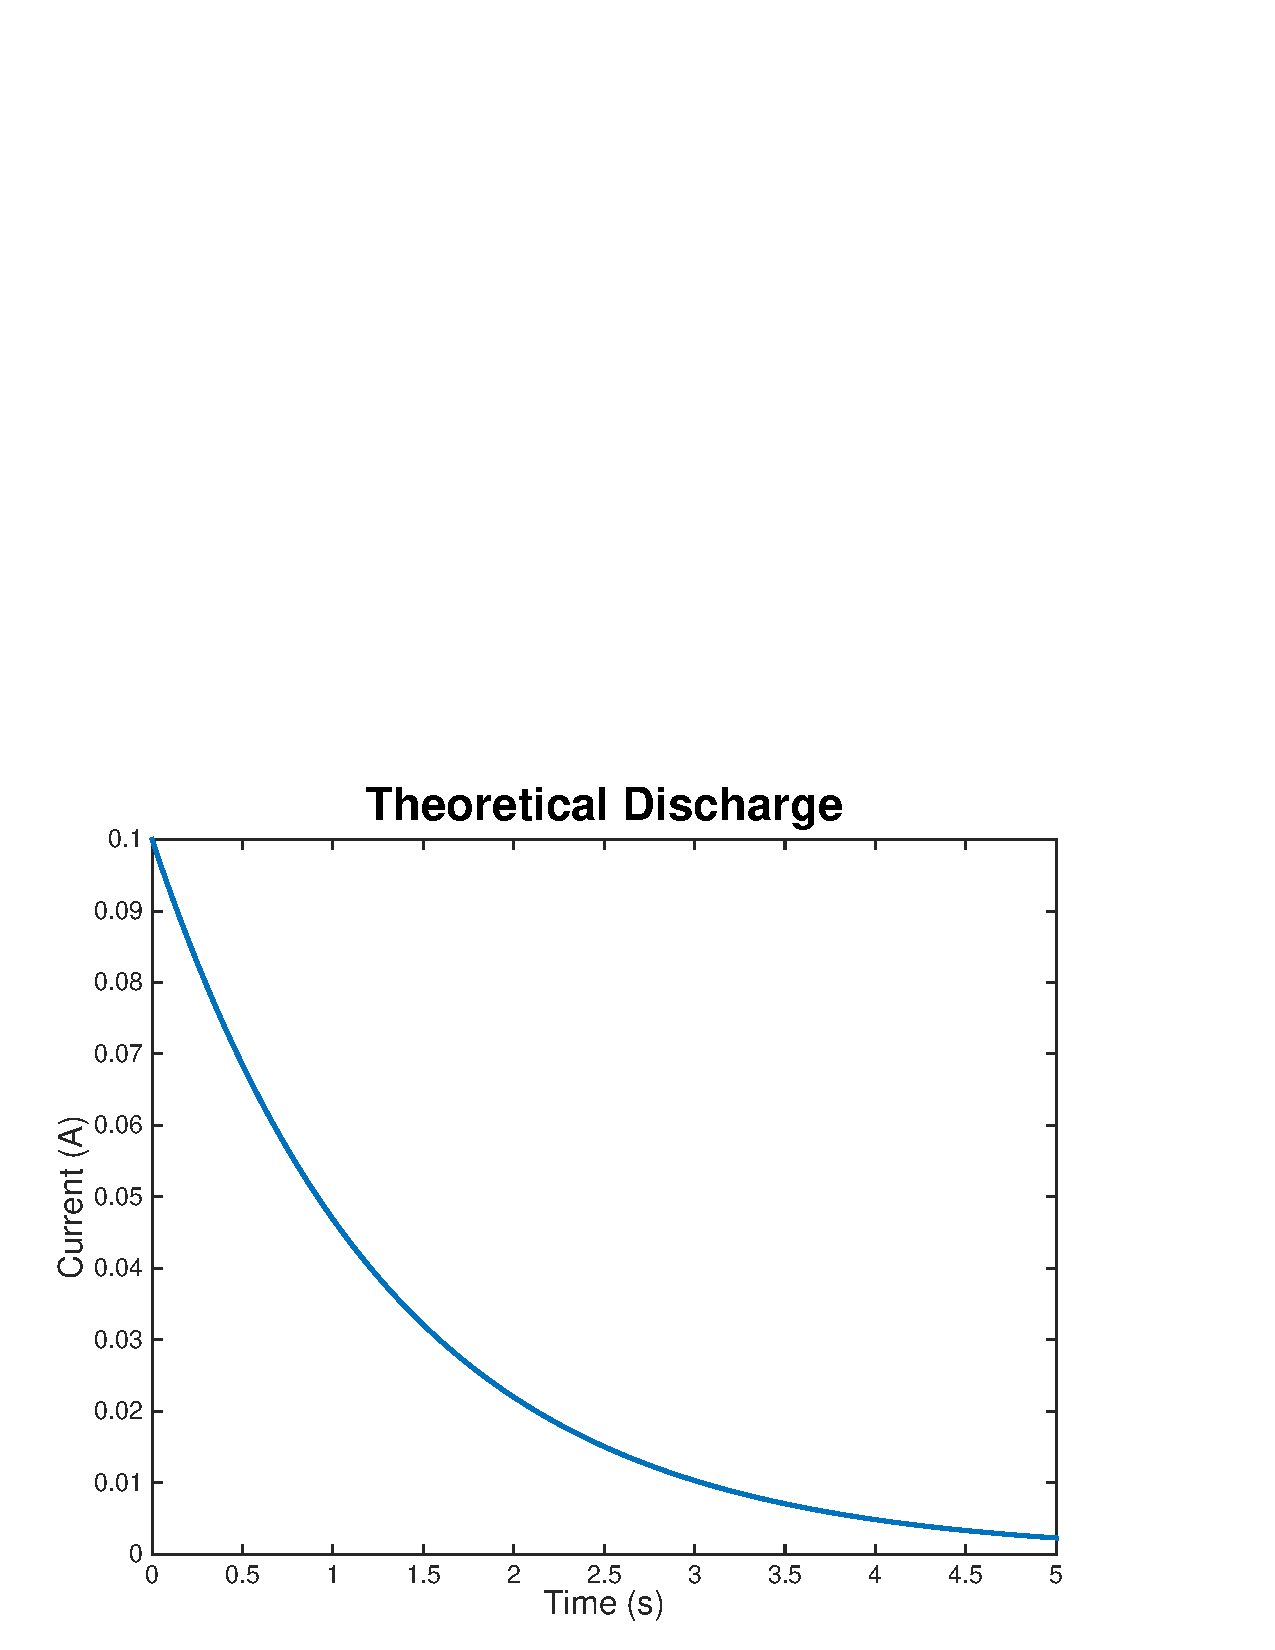
\includegraphics[width = 0.7 \textwidth]{discharge_current}
    \caption{Current of the theoretical discharge from \fref{fig:discharge_voltage}. This was computed using the voltage exponential and the equation $I = \frac{V}{R}$.}
    \label{fig:discharge_current}
\end{figure}

	\begin{table}[H]
		\centering
		\begin{tabular}{|l|l|}
		\hline
		Resistor type & Ohmite AP101 TO-247-2 \\ \hline
		Resistance & 3 k\ohm \\ \hline
		Continuous power rating & 100 W \\ \hline
		Overload power rating & 1.5 times rated power for 5 seconds \\ \hline
		Maximum expected current & 0.1 A \\ \hline
		Average current & 0.0261 A\\ \hline
		Cross-sectional area of the wire used & 0.83mm$^2$ (18 AWG) \\ \hline
		\end{tabular}
		\caption{General data of the discharge circuit}
		\label{dctable}
	\end{table}

\hl{The discharge relay is identical to the relay used for pre-charge and detailed in table {\ref{PCrelay}}. Note, as this is a SPDT relay, we can configure it to be normally open for pre-charge, and normally closed for discharge.}

\begin{figure}[H]
    \centering
    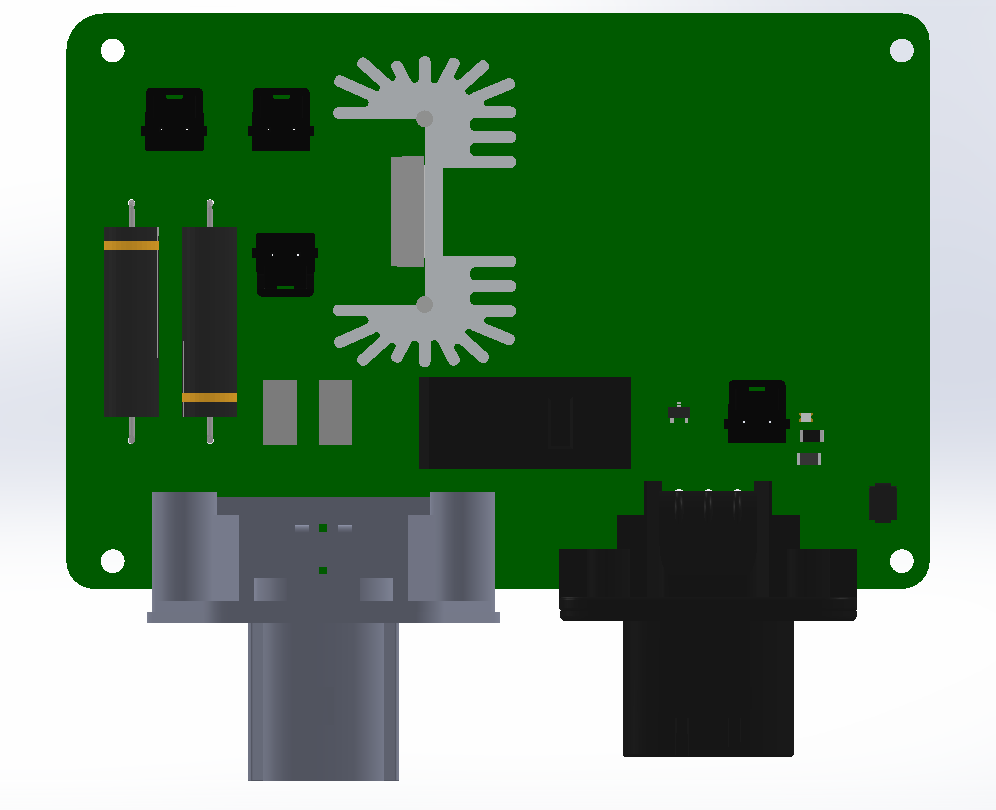
\includegraphics[width = 0.7 \textwidth]{discharge_pcb}
    \caption{\hlr{Render of the discharge circuit PCB. The discharge resistor is a TO-247 package mounted to a heatsink. }}
    \label{discharge_pcb}
\end{figure}

\hl{As shown in figure {\ref{discharge_pcb}} the discharge resistor is mounted to an Ohmite RA-T2X-51E heatsink. Figure {\ref{discharge_heat}} shows the modeled temperature of the discharge resistor under the maximum continuous discharge current for 15 seconds. This temperature curve was computed using the equation,}

\begin{equation}
    \Delta T = \frac{(P_{in} - P_{out}) \Delta t}{m*C_p}
\end{equation}

\hl{Where $P_{out}$ is the power dissipation of the heatsink given by, }

\begin{equation}
    P_{out} = \frac{1}{R_{therm}}(T-T_{amb}),
\end{equation}

\hl{$P_{in}$ is the power generated by the resistor, $\Delta t$ is the time step of the simulation, $m$ is the mass of the heatsink in kg, $C_p$ is the specific heat of aluminum, $R_{therm}$ is the thermal resistance of the heatsink under natural convection in $\frac{\degree C}{W}$, $T$ is the temperature of the heatsink, and $T_{amb}$ is the temperature of the ambient air. Code for this simulation can be found in the appendix section {\ref{appendix_discharge}}}




\begin{figure}[H]
    \centering
    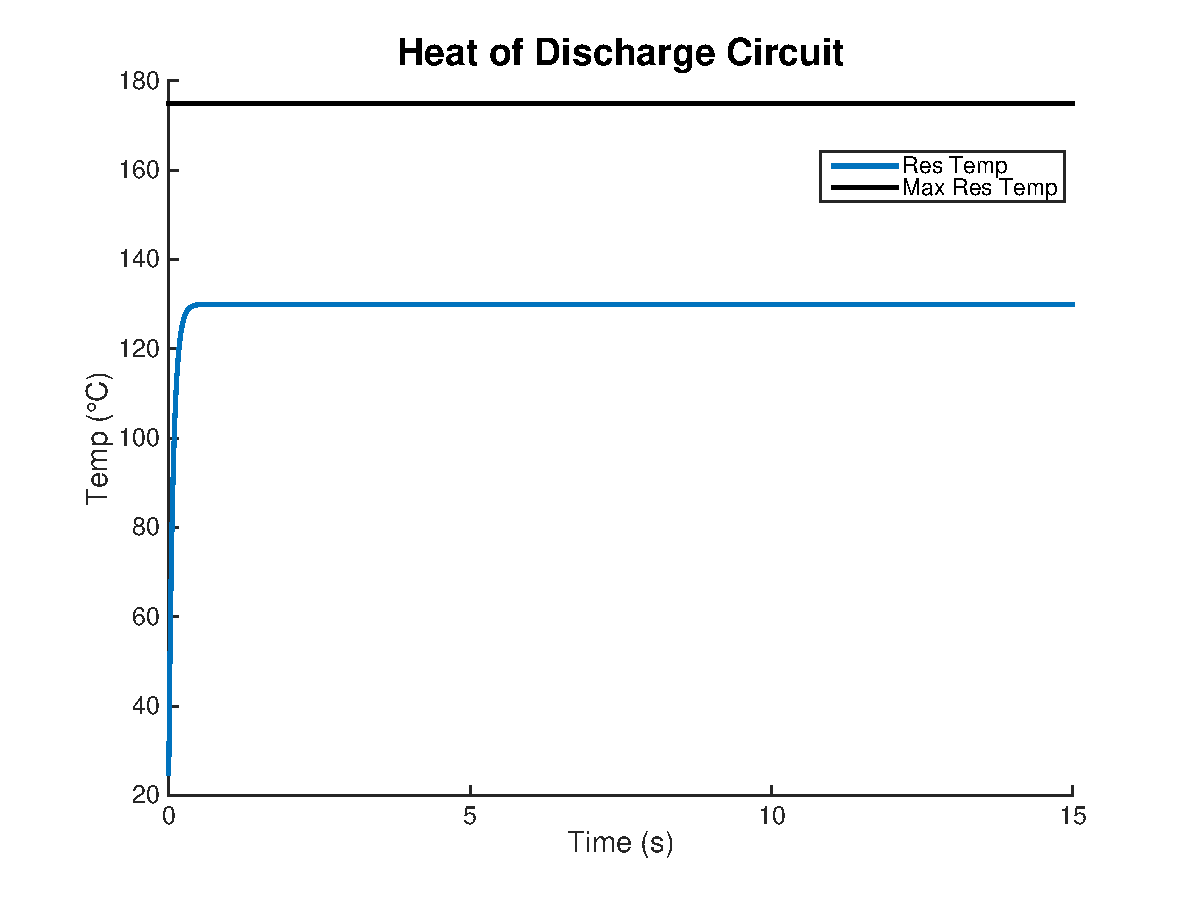
\includegraphics[width = 0.7 \textwidth]{discharge_heat_2}
    \caption{\hlr{Model of discharge resistor temperature under maximum continuous discharge current for 15 seconds.}}
    \label{discharge_heat}
\end{figure}



\subsubsection{Position in car}
%Provide CAD-renderings showing all relevant parts. Mark the parts in the rendering, if necessary.
The discharge circuit is located within the Energy Meter enclosure detailed in section \ref{energy_meter_mounting}, in close proximity to the motor controller which is the main capacitive load in the tractive system. 

\subsection{HV Disconnect (HVD)}\label{hv_disconnect}
\subsubsection{Description}
%Describe your concept of the HVD and how it can be operated.
We will be using the \hl{630A Fuse} version of a TE Connectivity AMP+ Manual Service Disconnect as our HVD. Shown in \fref{fig:TE_MSD}, it is a sealed, lever operated panel mount device and can be removed without tools. To protect technicians, it has no exposed conductors and provides internal HV interlocking in compliance with EV4.7.5. 

\begin{figure}[H]
\centering
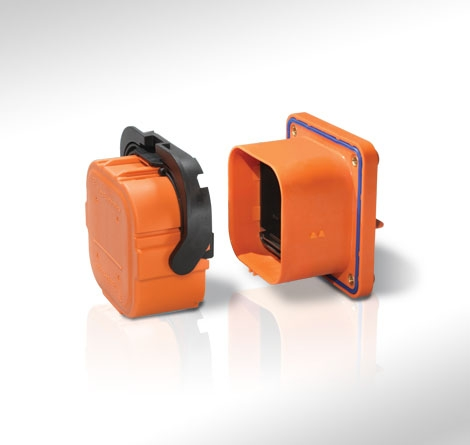
\includegraphics[scale=.7]{TE_Manual_Service_Disconnect.jpg}
\caption{The TE Manual Service Disconnect}
\label{fig:TE_MSD}
\end{figure}

\subsubsection{Wiring, cables, current calculations, connectors}
%Describe wiring, show schematics, describe connectors and cables and show useful data regarding the wiring.  Include information on the working voltage and current rating of the HVD.
The Manual Service Disconnect is rated for 495V and contains a 630A fuse, which is more than our maximum current of 225A as shown in \fref{tab:batterytable}. This fuse is superfluous to the TS main fuse, and is simply included as part of the disconnect.  It has a dual lever action, which first disconnects the shutdown circuit interlock inside the plug before disconnecting the high power terminals, which causes the AIRs to open and the tractive system to de-energize. The Manual Service Disconnect is a sealed panel mount device, which prevents the ingress of any water or debris. \\

The datasheet can be found in section \ref{appendix_hvd}.\\

The HVD is in series with the negative pole of the tractive system, on the vehicle side of the AIRs, as shown in \fref{fig:TS_block_diagram}. 

\subsubsection{Position in car}
%Provide CAD-renderings showing all relevant parts. Mark the parts in the rendering, if necessary.
The HVD is mounted at the rear of the vehicle, on the rear-facing side of the energy meter enclosure, however this enclosure is yet to be designed. It is bright orange, and will be clearly marked and easily accessible from the rear of the vehicle. In accordance with EV 4.7.1, the HVD will be mounted more than 350mm from the ground.  

\begin{figure}[H]
\centering
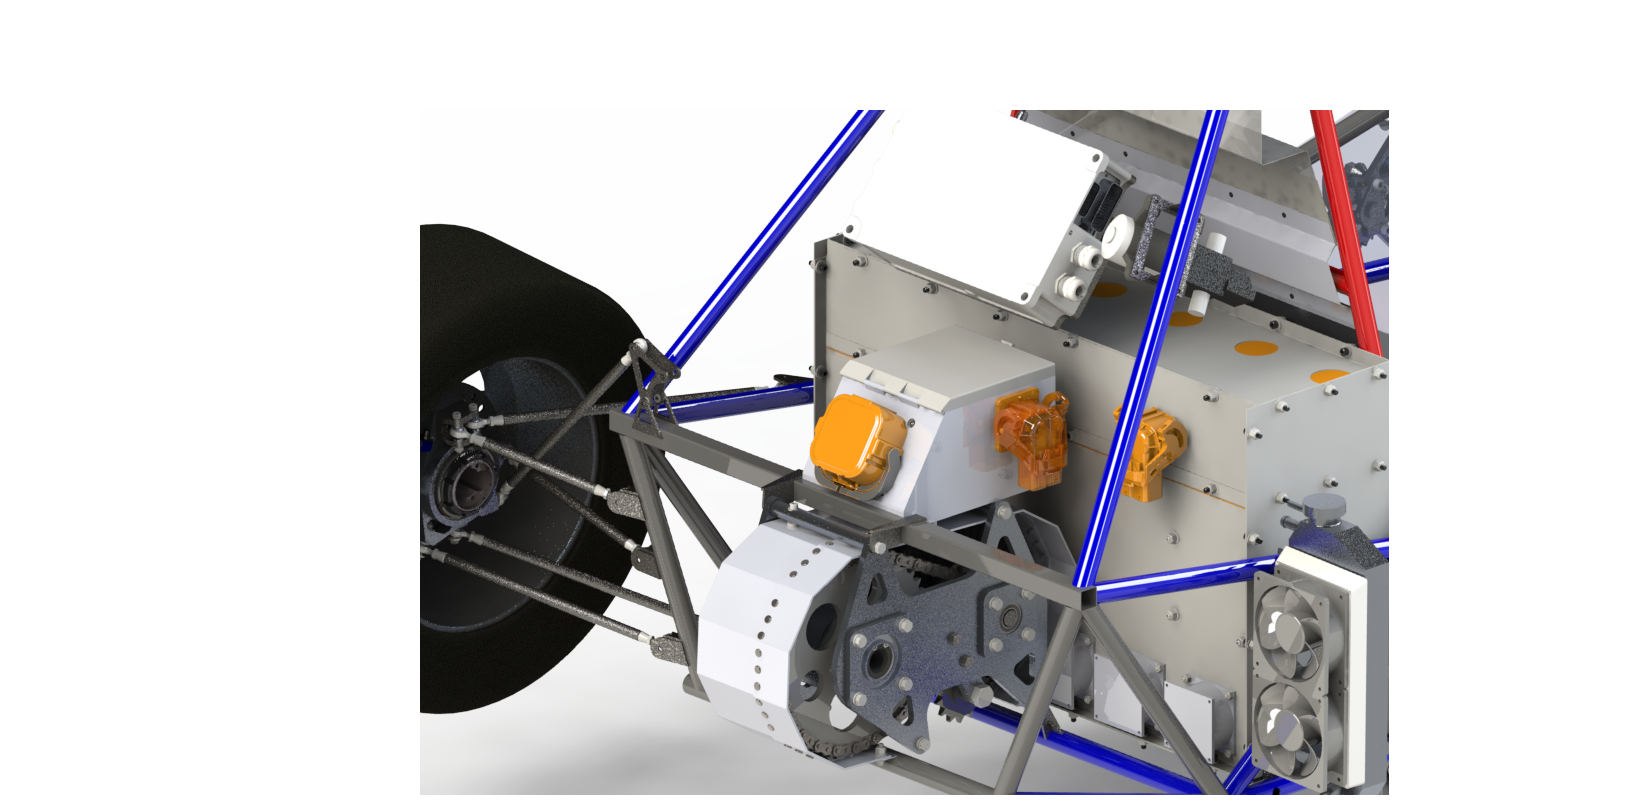
\includegraphics[width=.75\textwidth]{EnergyMeterBackISO}
\caption{The HVD's location in the car.}
\label{fig:hvd}
\end{figure}

\hlr{As seen in} \fref{fig:hvd_side}\hl{, the HVD mounting on the energy meter enclosure is currently in violation of EV4.2.1. This is not a final configuration, and the enclosures team is currently redesigning this enclosure and its mounting to move the HVD entirely within the chassis envelope.}

\begin{figure}[H]
\centering
\includegraphics[width=.75\textwidth]{EnergyMeterBackOfCar}
\caption{\hlr{a side view of the HVD mounting, showing protrusion from the chassis envelope. This is a temporary state, and will not be reflected in final design}}
\label{fig:hvd_side}
\end{figure}


\subsection{Ready-To-Drive-Sound (RTDS)}\label{ready_to_drive_sound}
\subsubsection{Description}
%Describe your concept of the RTDS, how is the sound produced, what are the parameters for activating the RTDS, etc.
The Ready to Drive sound is located as a component of the dashboard subsystem, and contains a buzzer (\href{http://www.mallory-sonalert.com/specifications/STA20502.PDF}{Link: Mallory Sonalert Products Inc. STA20502})\ref{Ready to Drive}. The buzzer  makes a noise when given a square wave at 1.25kHz, with the loudness proportional
to the voltage. When the shutdown sequence is complete, a message will be sent out over the CAN bus \hl{from the Master Switch Panel monitor PCB, alerting the Dashboard CAN node to wait for the start sequence. The start sequence consists of pressing the brake pedal and then the start button while the shutdown circuit is entirely closed. The dashboard will} then provide the 1.25kHz wave to the gate of an N-FET which will provide a ground path for the buzzer. \hl{To prompt the driver, the start button will not illuminate until the shutdown circuit is closed and the brake pedal is pressed.}
\subsubsection{Wiring, cables, current calculations, connectors}
%Describe wiring, show schematics, describe connectors and cables and show useful data regarding the wiring.
\hl{Once the vehicle is in ready to drive mode, the dashboard CAN node} will activate the ready to drive sound node to \hl{drive the N-FET high} for 2 seconds, thus letting the buzzer sound for 2 seconds. 


\begin{figure}[H]
	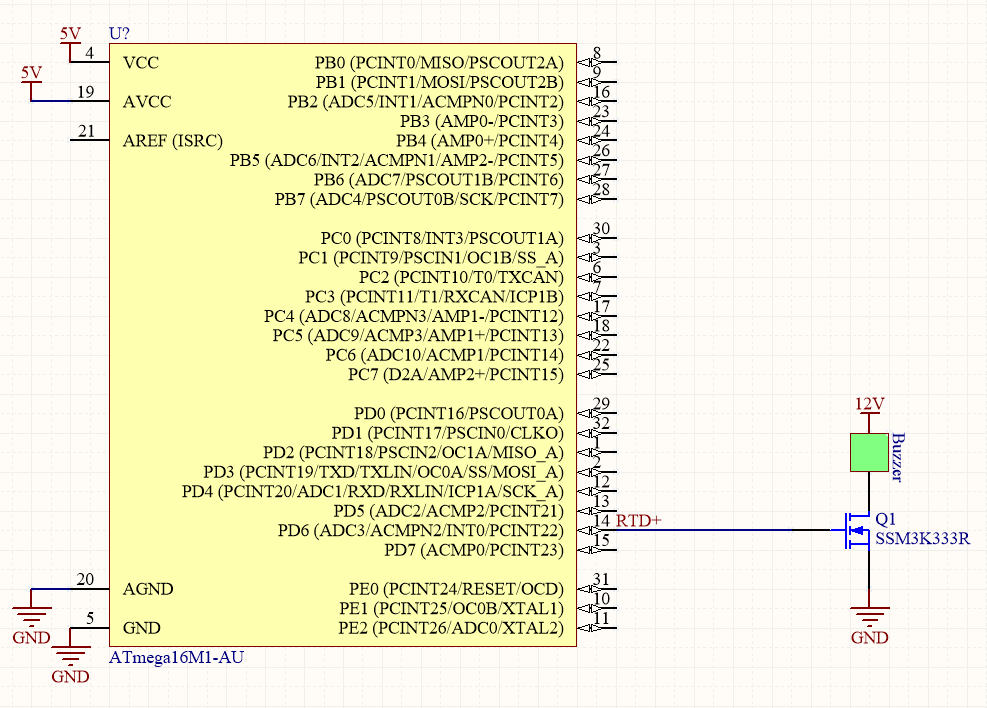
\includegraphics[width=\linewidth]{RTDS_Schematic_Simplified}
	\caption{Ready to Drive Sound Schematic as a subsystem of the dashboard's PCB}
\end{figure}
\begin{figure}[H]
\centering
	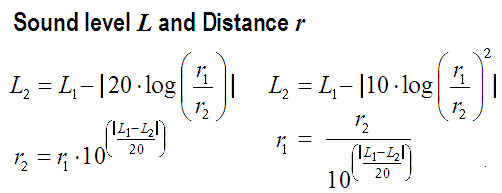
\includegraphics[width=0.6\linewidth]{FormulasForDistanceAndSoundLevel}
	\caption{Inverse Square Law equations needed to calculate the volume at a certain distance}
\end{figure}
Using the inverse square law as referenced in the appendix  for sound pressure levels \ref{Ready to Drive}, 97db at 122cm will translate to 93db at 2m which is a loud enough volume without inducing harm to the listener. 
\subsubsection{Position in car}
%Provide CAD-renderings showing all relevant parts. Mark the parts in the rendering, if necessary.
The ready to drive sound will be located in the dashboard enclosure. The buzzer will be mounted
to the exterior and front side of this enclosure, facing the front of the car as seen in figure \ref{dashboard_right}. It must be contained outside of the box so that the buzzer is
loud enough. The speaker is waterproof, so it doesn't require any extra protection besides using an RTV silicone seal for final installation. 

\begin{figure}[H]
\centering
	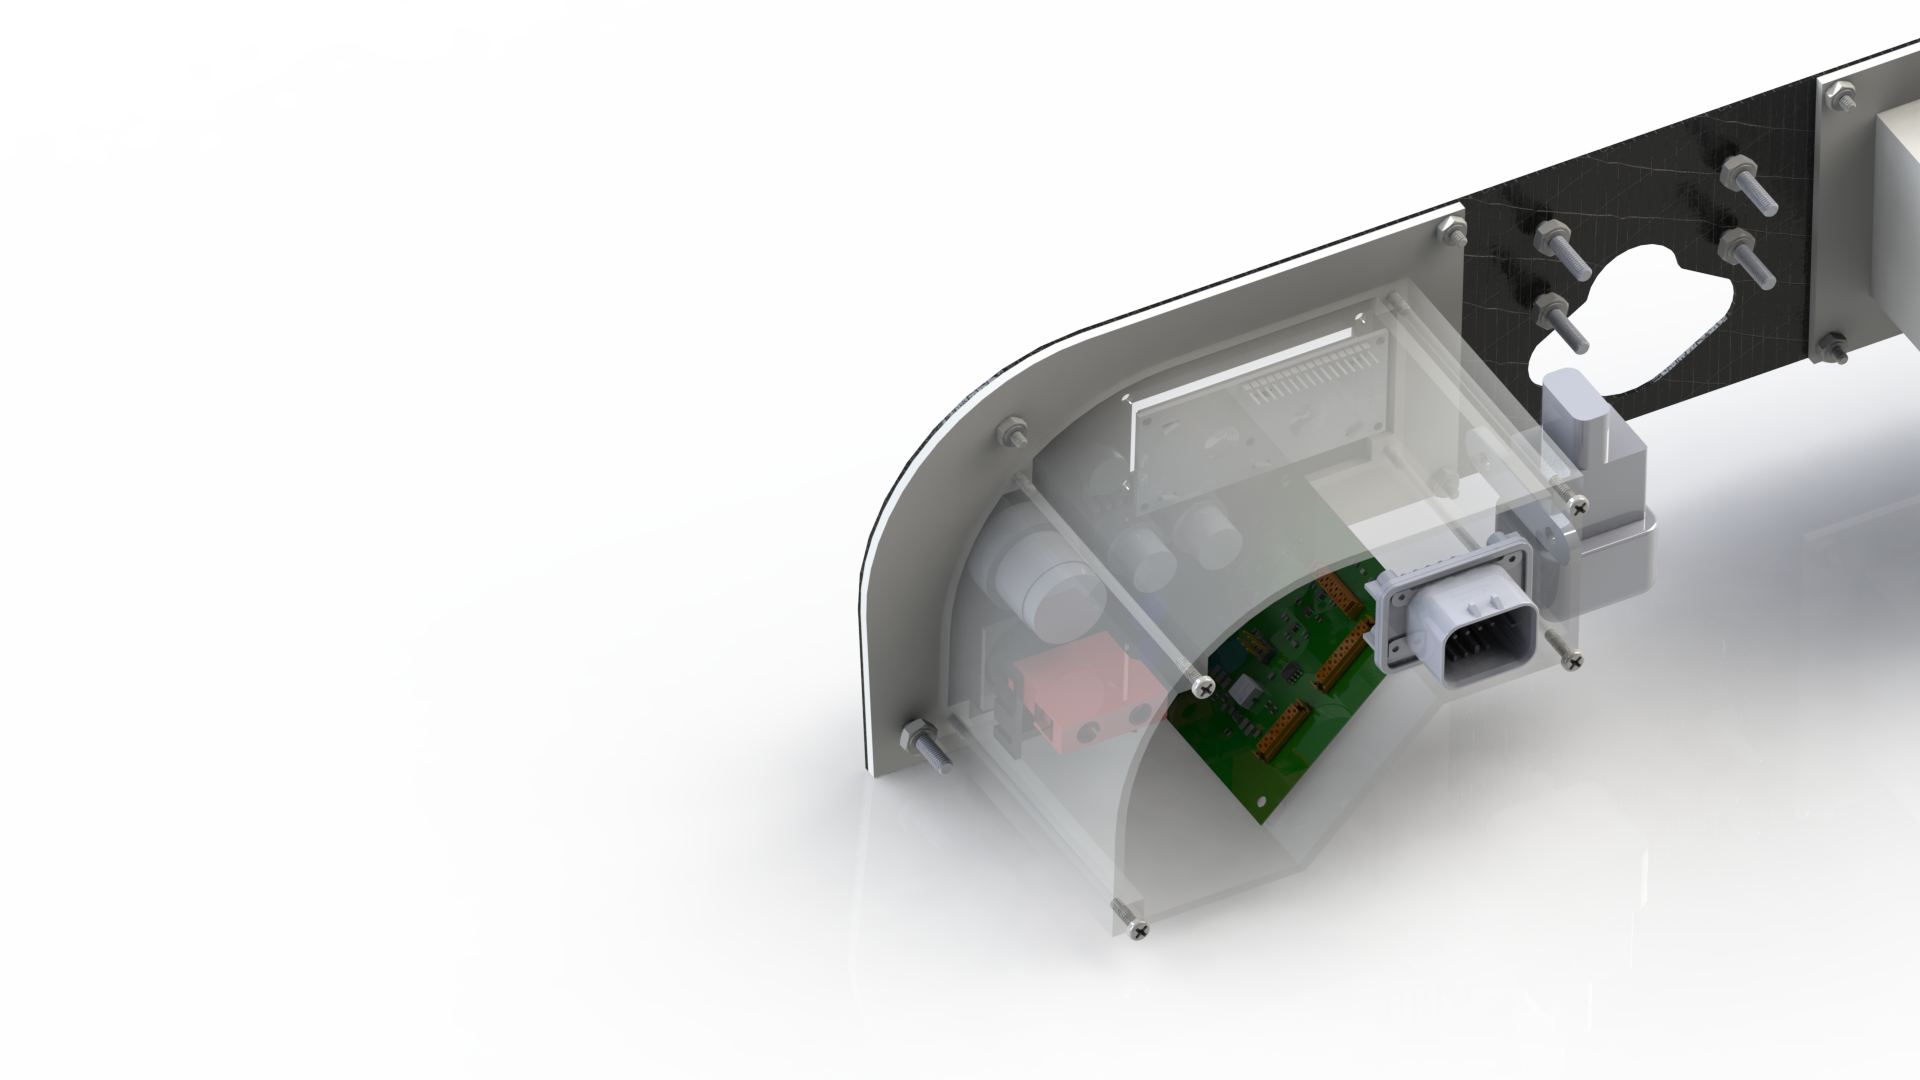
\includegraphics[width=0.6\linewidth]{dashboard_right}
	\caption{Rendering of Dashboard Right}
	\label{dashboard_right}
\end{figure}


\section{Accumulator}\label{accumulator}
\subsection{Accumulator pack 1}\label{accumulator_pack_1}
\subsubsection{Overview/description/parameters}\label{accumulator_overview}
%Describe concept of accumulator pack, provide table with main parameters like number of cells, cell stacks separated by maintenance plugs, cell configuration, resulting voltages->minimum, maximum, nominal, currents, capacity etc.

The accumulator pack is based on 72 \hl{A123 AMP20M1HD-A LiFePO4} pouch cells, in a 72s1p configuration. It is divided into six segments of 12 cells each, which each have their own distributed voltage and temperature management systems that communicate to a master BMS node that interacts with the car's CAN network and can open the shutdown circuit. Each cell has nominal characteristics seen in \fref{tab:cells}, and together they form an accumulator with a max voltage of \hl{259.2 V}, and a max output current of \hl{600 A}, with \hl{25.9 MJ} total capacity. Details can be found in \fref{tab:batterytable}.  


	\begin{table}[H]
	    \centering
	    \begin{tabular}{|l|l|}
	        \hline
	        Maximum Voltage & \hl{259.2 VDC} \\ \hline
	        Nominal Voltage & \hl{237.6 VDC} \\ \hline
	        Minimum Voltage & \hl{144 VDC} \\ \hline
	        Maximum output current & \hl{600 A (10s Pulse)} \\ \hline
	        Maximum nominal current & \hl{200 A} \\ \hline
	        Maximum charging current & \hl{100 A} \\ \hline
	        Total number of cells & 72 \\ \hline
	        Cell configuration & 72s1p \\ \hline
	        Total capacity & \hl{25.9 MJ} \\ \hline
	        Number of cell stacks (segments) & 6 \\ \hline
	    \end{tabular}
	    \caption{Main accumulator parameters}
	    \label{tab:batterytable}
	\end{table}

\begin{figure}[H]
\centering
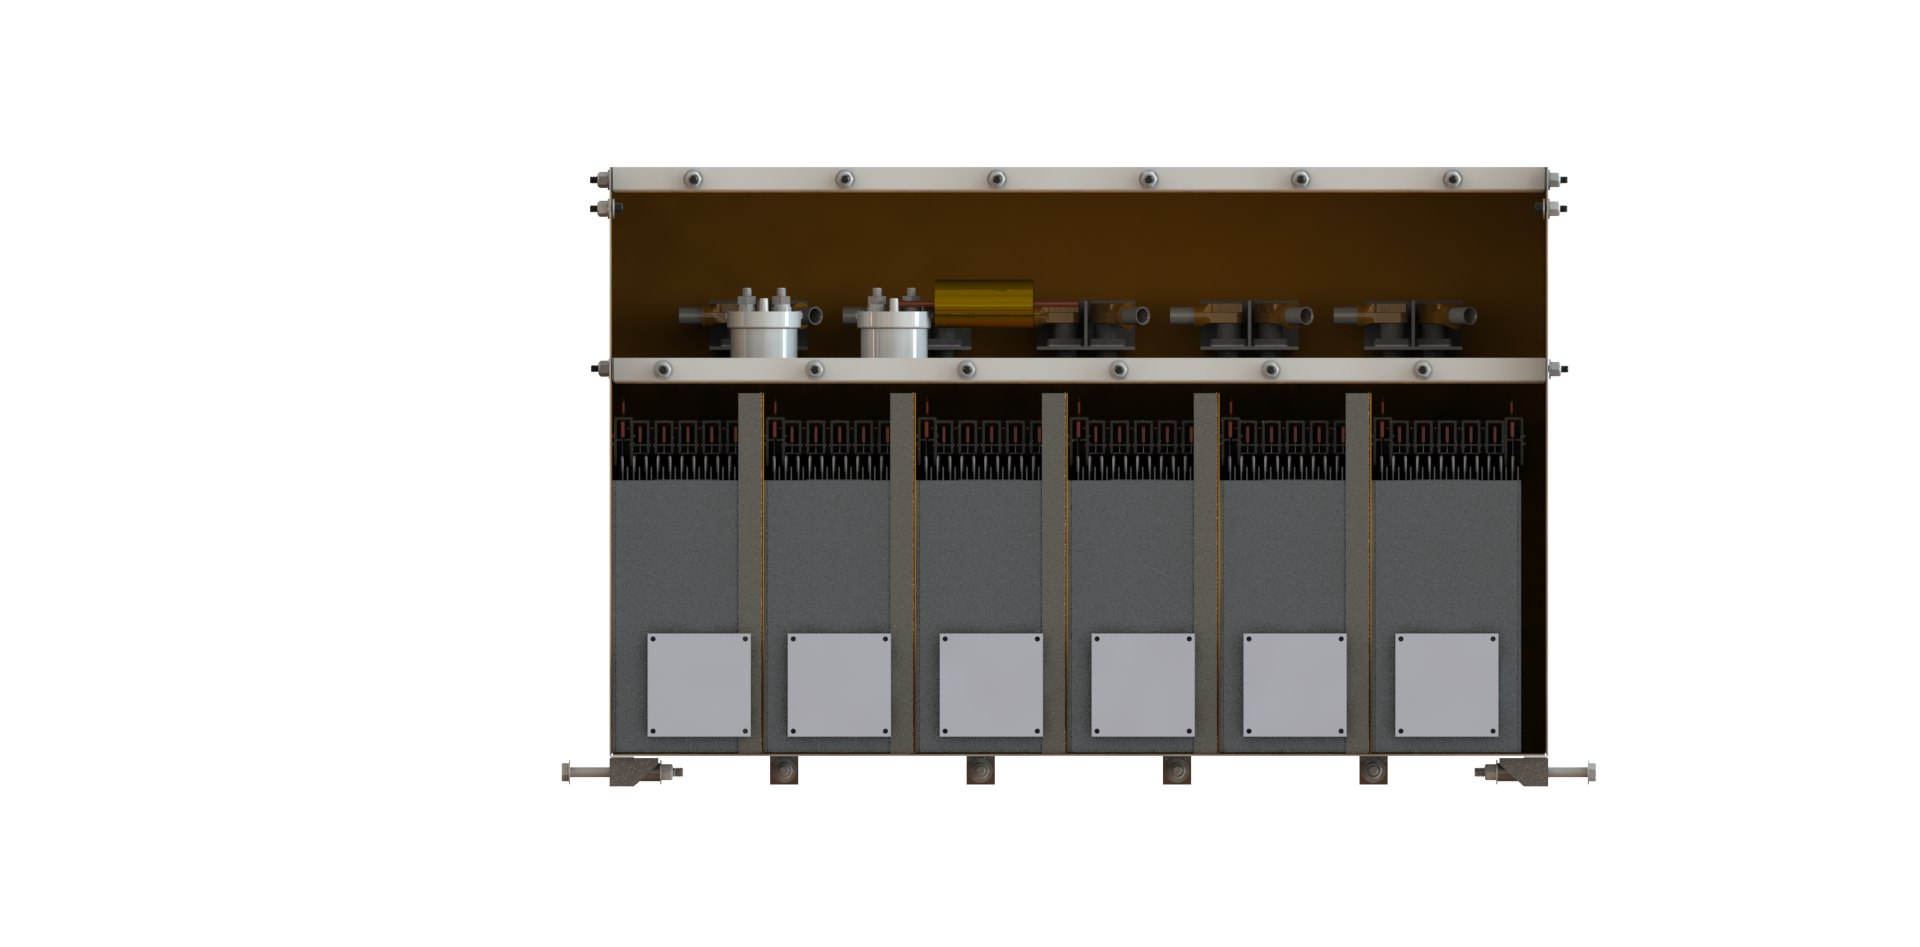
\includegraphics[width=1\textwidth]{accumulator_front}
\caption{\hl{Render of the accumulator with one panel removed to show cell arrangement.}}
\label{fig:accumulator_hero}
\end{figure}

\subsubsection{Cell description}\label{accumulator_cell_description}
%Describe the cell type used and the chemistry, provide table with main parameters.

The cells we are using are LG Chem Model P2.7, which are lithium nickel manganese cobalt oxide (NMC) pouch cells. The relevant values from the datasheet are shown in \fref{tab:cells}.


	\begin{table}[H]
	    \centering
	    \begin{tabular}{|l|l|}
	        \hline
	        Cell Manufacturer and Type &
	            \begin{tabular}[c]{@{}l@{}}
	                LG Chem\\ Model P2.7
	            \end{tabular} \\ \hline
	        Cell nominal capacity & 25.9 Ah \\ \hline
	        Maximum Voltage & 4.15 V \\ \hline
	        Nominal Voltage & 3.7 V \\ \hline
	        Minimum Voltage & 2.8 V \\ \hline
	        Maximum output current & 225 A \\ \hline
	        Maximum nominal output current & 125 A \\ \hline
	        Maximum charging current & 180 A \\ \hline
	        Maximum Cell Temperature (discharging) & 45\degree C \\ \hline
	        Maximum Cell Temperature (charging) & 45\degree C \\ \hline 
	        Cell Chemistry & NMC/LMO\\ \hline
	    \end{tabular}
	    \caption{Main cell specification}
	    \label{tab:cells}
	\end{table}

\subsubsection{Cell configuration}\label{accumulator_cell_configuration}
%Describe cell configuration, cell interconnect, show schematics of electrical configuration and CAD of connection techniques, cover additional parts like internal cell fuses etc.
The P2.7 pouch cells are connected in six segments of 12 cells in series, for a total configuration of 72s1p, as shown in \fref{fig:cell_configuration_schematic}. 

\begin{figure}[H]
\centering
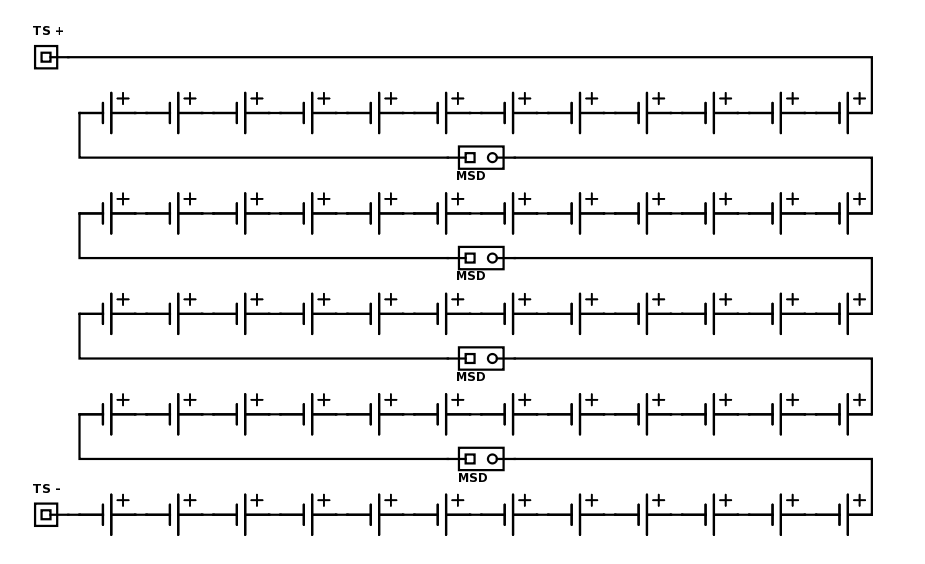
\includegraphics[width=0.6\textwidth]{Cell-configuration-schematic.png}
\caption{A schematic of the accumulator's cell configuration showing cells in series and manual service disconnects}
\label{fig:cell_configuration_schematic}
\end{figure}

To connect the cells into segments, they are stacked on one another with 1mm 6061 aluminum heat sinks and neoprene compression foam to distribute load. The cells are alternated in polarity for easy tab connection. Data on the foam can be found in the appendix, in section \ref{appendix_accumulator_cell_configuration}.

\hl{Individual cells are connected by squeezing their tabs together with bolted copper plates. Voltage sensing is done using wires connected to these plates. Each bolted plate assembly is isolated with a 3d-printed cover. This cover protects each terminal from shorts during assembly and maintenance. Each cover is retained with a zip-tie. This is a safer assembly technique than welding the cell tabs together, and allows for replacement of damaged cells if necessary.} 

\begin{figure}[H]
\centering
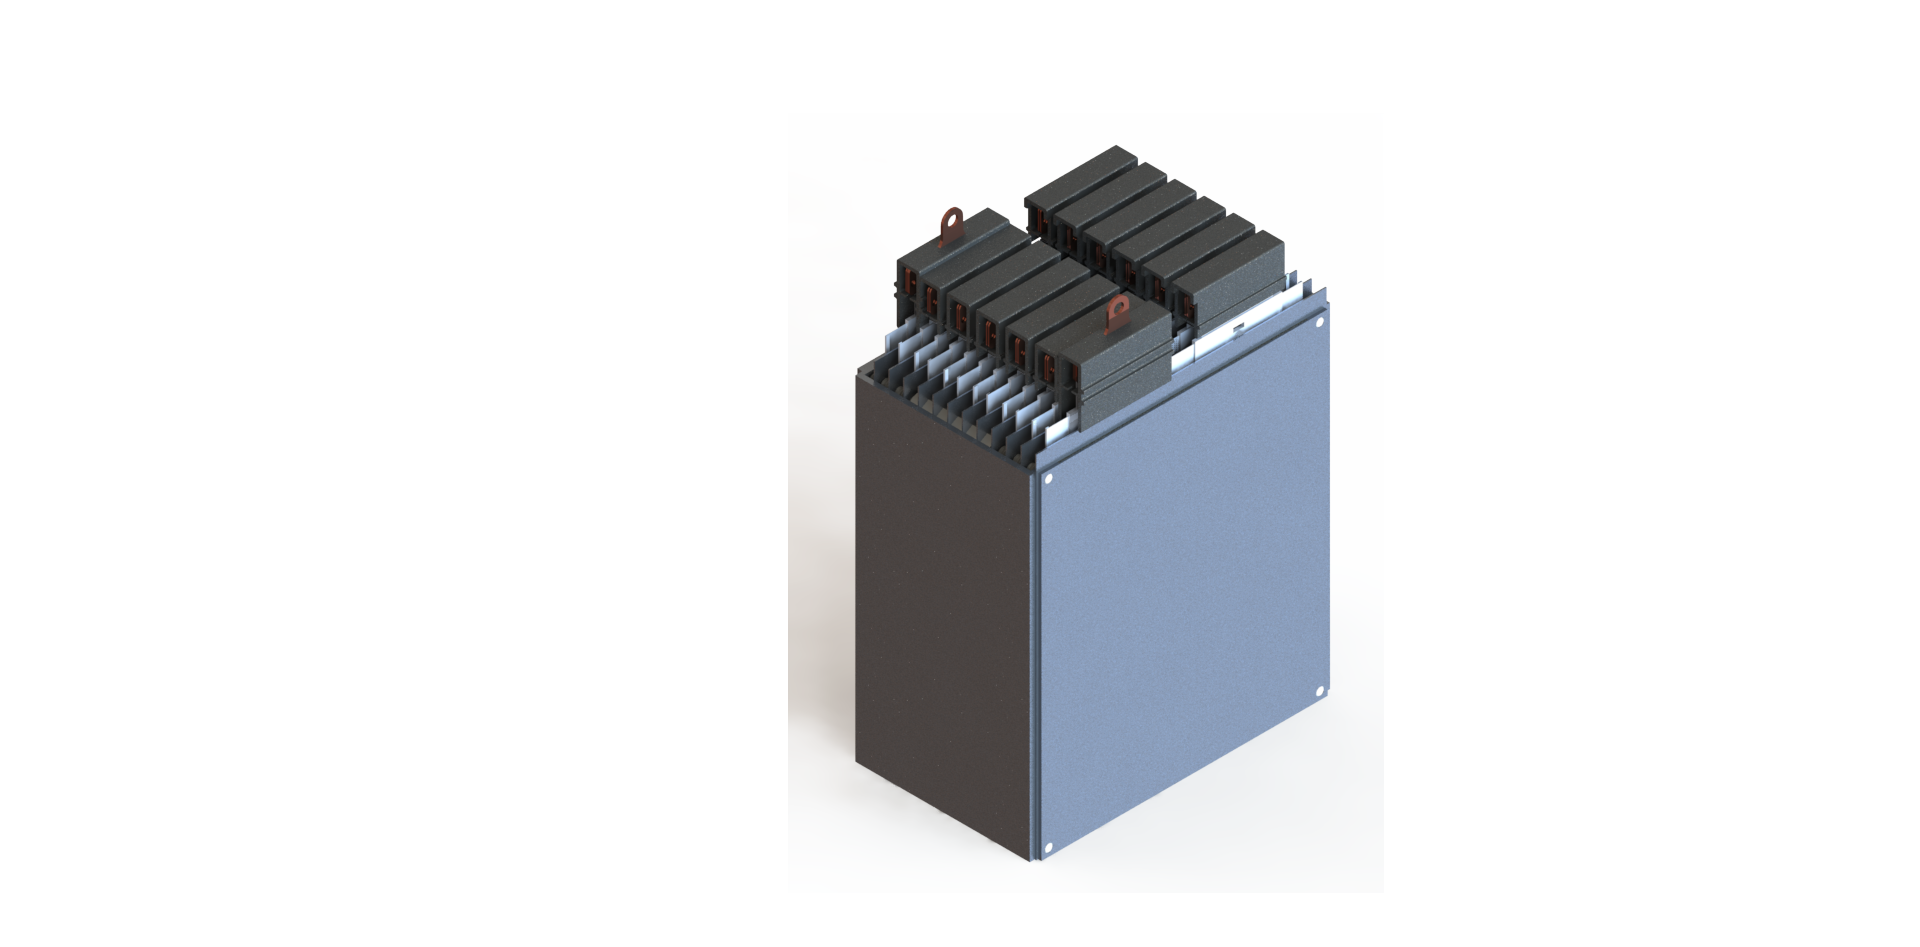
\includegraphics[width=1\textwidth]{module_iso_method_2}
\caption{\hl{Single segment of 12 cells with 3d-printed covers over clamped cell tabs.}}
\label{fig:cell_tabs}
\end{figure}

In between the segments, there will be a 4AWG jumper made of the vehicle's HV cable, with a 1-position connector on each end. These will be on the tops of the cell segments, and will be easily removable, so as to act as the manual service disconnects between segments. We are currently in communication with sales representatives from Amphenol about an appropriate connector for our application, and we are considering the Radlok connector system, seen in \fref{fig:radlok}.

\begin{figure}[H]
\centering
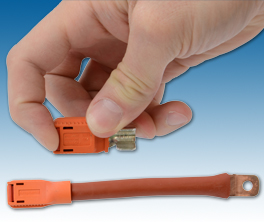
\includegraphics[width=0.6\textwidth]{RADLOK-main.jpg}
\caption{Radlok connector example. The product page can be found \href{http://www.amphenol-industrial.com/radlok}{here}}
\label{fig:radlok}
\end{figure}


\subsubsection{Cell temperature monitoring}\label{accumulator_cell_temperature_monitoring}
%Describe how the temperature of the cells is monitored, where the temperature sensors are placed, how many cells are monitored, etc. Show schematics, cover additional parts, etc.

In compliance with EV3.6.3 and EV3.6.6 the temperature of every cell will be measured within \hlr{10mm} of the negative terminal. We will achieve this by \hl{epoxying} an NTC thermistor to the insulated section of the negative terminal of each cell, as close as possible to the body of the cell. The thermistors will be electrically isolated from the terminal by the insulating foil of the cell, and the temperature measurement will most closely approximate the internal temperature of the electrode by being close to the body of the cell. 

\begin{figure}[H]
    \centering
    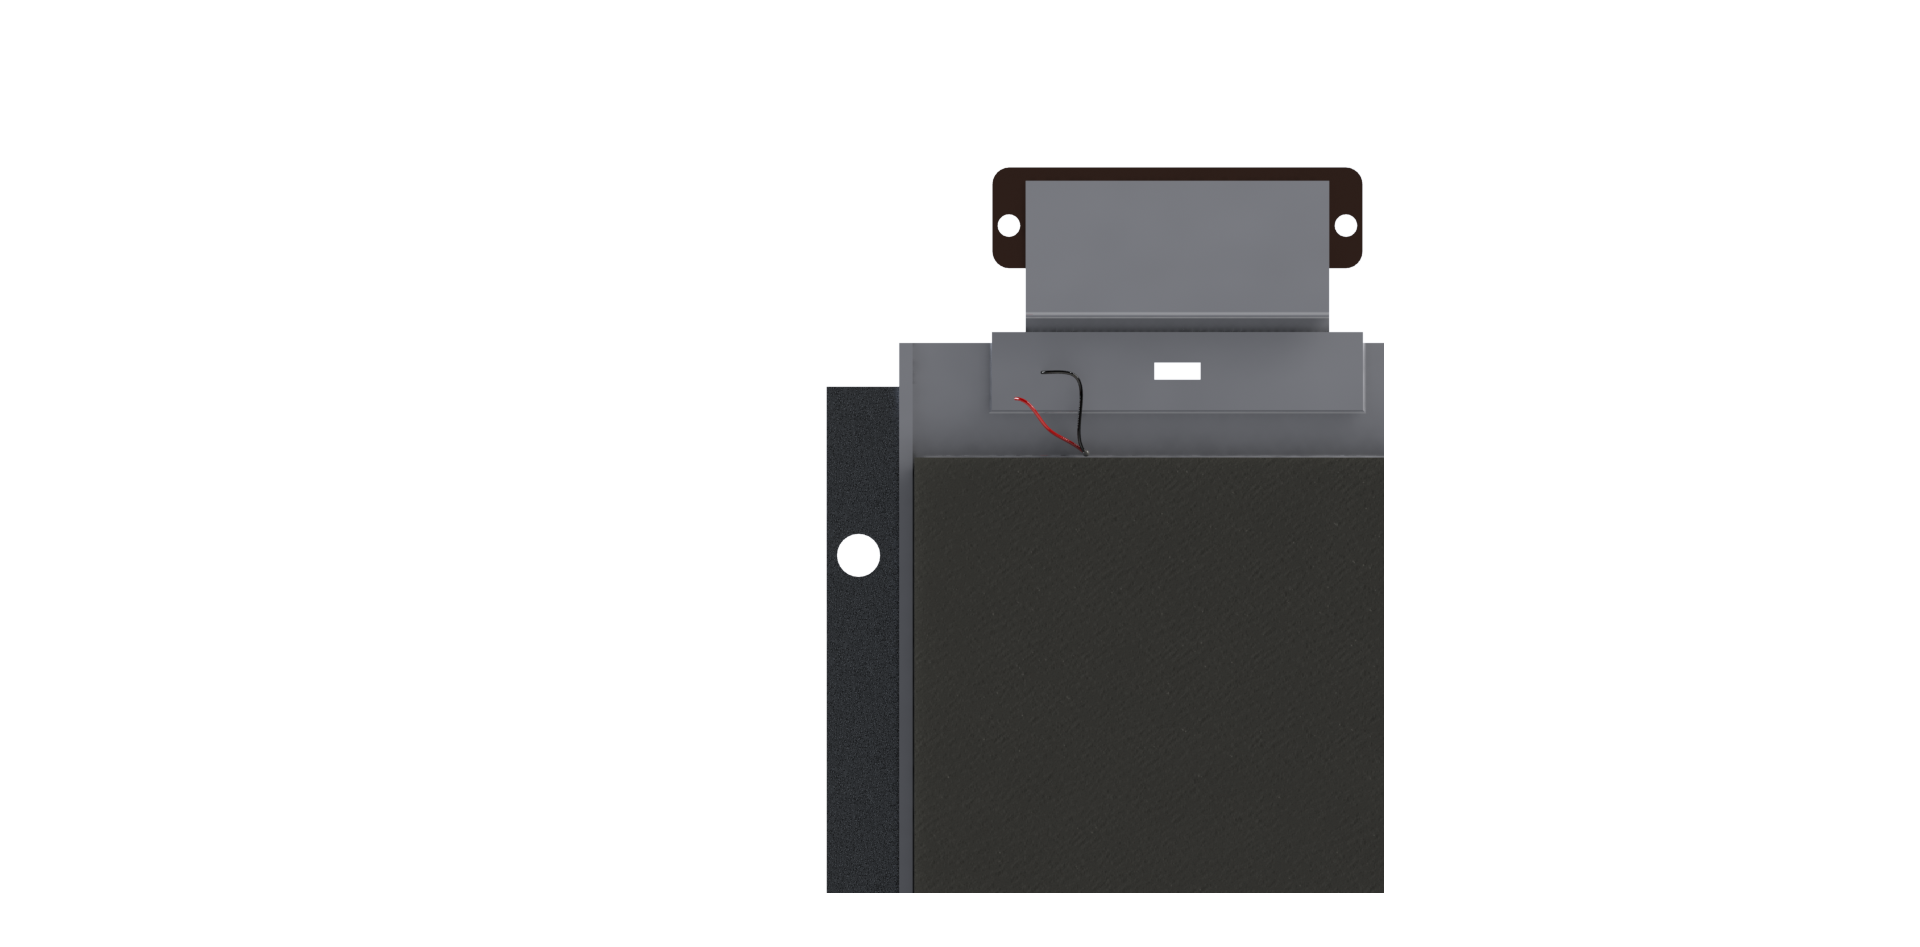
\includegraphics[width=1\textwidth]{thermistor}
    \caption{\hl{Approximate positioning of the thermistors (seen here with red and black leads) relative to the cells}}
    \label{fig:cell_temp_monitor}
\end{figure}

\begin{figure}[H]
    \centering
    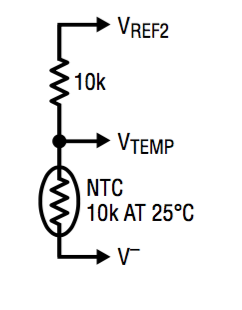
\includegraphics[width=0.2\textwidth]{therm_circuit}
    \caption{Circuit for sensing NTC thermistors}
    \label{fig:therm_circuit}
\end{figure}

\begin{figure}[H]
    \centering
    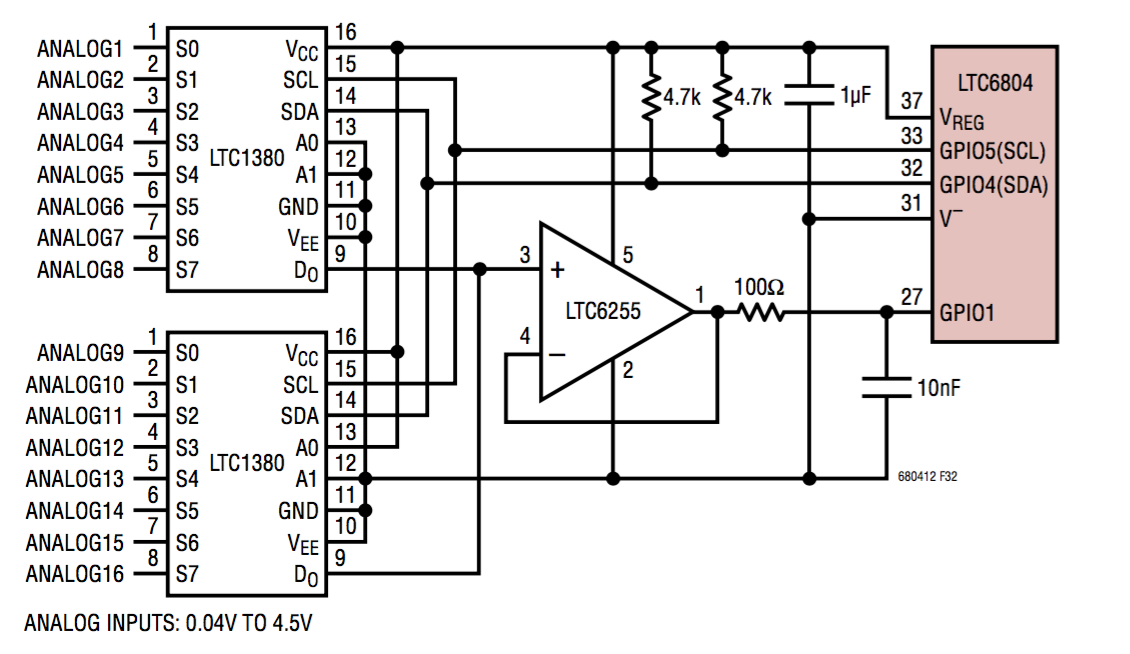
\includegraphics[width=0.8\textwidth]{mux_circuit}
    \caption{Circuit for multiplexing analog inputs for LTC6804 BMS chip}
    \label{fig:mux_circuit}
\end{figure}

The NTC thermistors are electrically connected in a voltage divider as shown in \fref{fig:therm_circuit}. Each of the temperature measurement voltages are multiplexed into a single GPIO pin on the LTC6804. See \fref{sec:accumulator_battery_management_system} for a more detailed description of the implementation of the LTC6804 BMS. 

The maximum cell operating temperature is 45 \textdegree C. Our thermistors are 1\% accurate, and the total measurement error of the ADC is $<$0.1\%, then in the worst case we will be reading 44.5 \textdegree C when the temperature is actually over the rating. To give the system a small safety margin, the BMS triggers a shutdown if it ever detects a cell temperature of 44 \textdegree C or higher. 


\subsubsection{Battery management system}\label{sec:accumulator_battery_management_system}
%Describe the BMS used including at least the following:
%-	Sense wiring protection (fusing / fusible link wire used)
%-	What upper and lower voltage does the BMS react at and how does it react?
%-	What cell temperature does the BMS react at and how does it react?
%-	Show tables of operation parameters
%-	Describe how many cells are sensed by each BMS board, the configuration of the cells, the configuration of the boards and how any comms wiring between boards is protected 
%-	Describe how the BMS is able to open the AIRs if any error is detected
%-	Describe where galvanic isolation occurs between TS and GLV system connections.

Each segment of the accumulator will be monitored and controlled for faults by its own distributed battery management system, which in turn communicates with a central master BMS that calculates state of charge, state of health, and monitors power consumption. In the case of a critical fault, the distributed segment BMS will send error messages over CAN to the master BMS, which has a relay that can open the shutdown circuit. In order to ensure that all segments remain in working order, the master BMS will employ a software watchdog timer, which will shut down the car if it fails to receive communication of nominal operation from each segment after a period of time. 

The distributed segment BMS is implemented using the Linear Technology LTC6804-1, which communicates over a daisy-chain-able galvanically-isolated SPI interface called isoSPI. The LTC6804 is capable of measuring the voltages of up to 12 lithium-ion batteries, and is also capable of measuring up to 16 analog inputs with its analog multiplexer. We are using the analog inputs to measure cell temperatures as referenced in section \ref{accumulator_cell_temperature_monitoring}. The LTC6804 datasheet can be found in the appendix under section \ref{appendix_accumulator_temperature}. 

\begin{figure}[H]
    \centering
    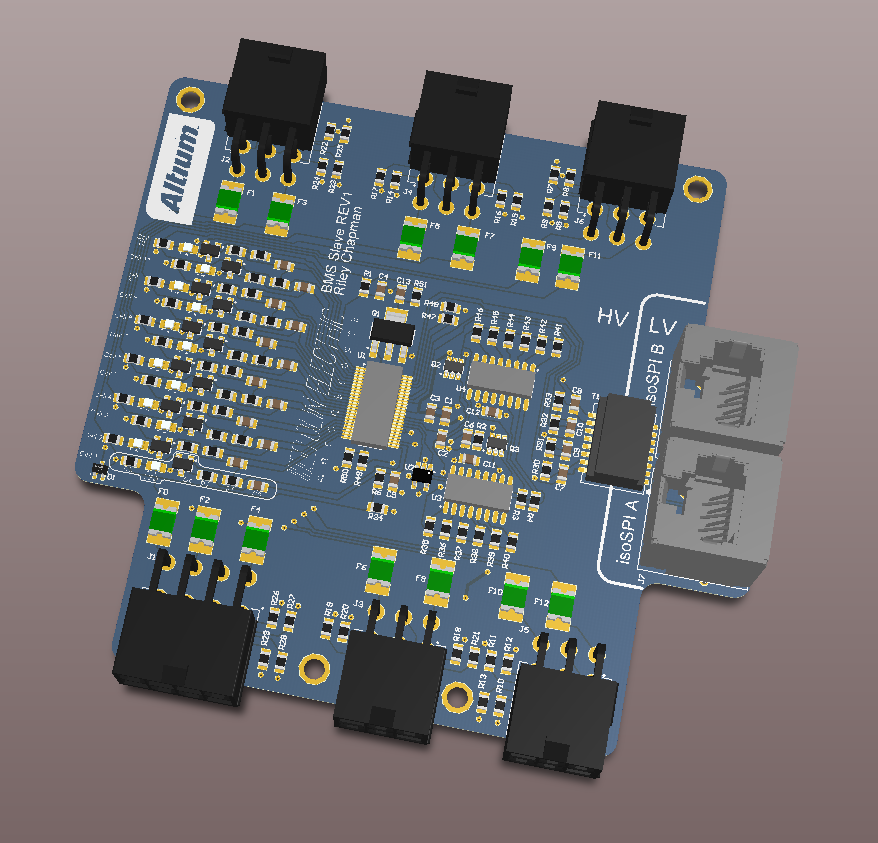
\includegraphics[width=1\textwidth]{BMS_slave_iso}
    \caption{\hl{Render of the LTC6804-1 based distributed segment BMS.}}
    \label{fig:BMS_slave_iso}
\end{figure}

\begin{figure}[H]
    \centering
    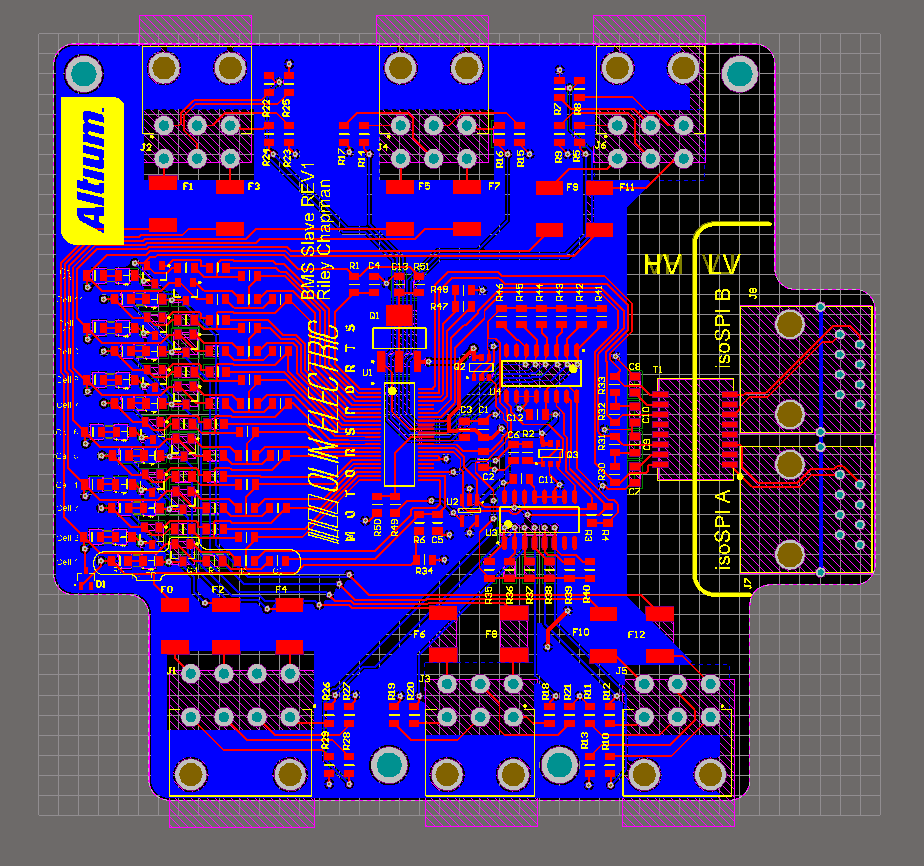
\includegraphics[width=0.8\textwidth]{BMS_slave_2D}
    \caption{\hl{Two dimensional view of distributed segment BMS.}}
    \label{fig:BMS_slave_2D}
\end{figure}

Communication wiring between the distributed segment BMS boards and the master BMS is achieved in a daisy chain via isoSPI, which terminates on the master BMS with an isoSPI interpreting ICs. The communication wiring will be properly retained to maintain spacing of 30mm from any TS voltage. 

The master BMS will be a node on the vehicle's CAN system, implemented using an ATmega16m1, a robust CAN-enabled automotive microcontroller. Its primary duties are measuring current leaving the pack via current-sensing coils, estimating state of charge and state of health, and opening the shutdown circuit if the distributed BMS boards sense a fault or fail to report nominal operational parameters. 

The maximum Total Measurement Error (TME) of the LTC6804 is 1.2 mV, so in order to account for this error, the max voltage the BMS will react to is 4.1488V, and the minimum voltage is 2.8012V. 

The BMS reacts to an upper voltage of 4.100V when charging by shunting excess power from that cell across a discharge resistor. This gives us a 48.8 mV leeway before we approach the max voltage of the cell, corrected for the maximum TME of 1.2 mV. If any cells ever reach 4.1488 V, the BMS will shut down the car by opening the shutdown circuit. This could occur during charging or regeneration in a rare case. 

The BMS reacts to critical low voltage of 2.8012V by shutting down the vehicle. This case is harder to remedy, because we can't recharge individual cells on the fly, so to avoid damaging the electrodes inside the cells, the BMS opens the shutdown circuit and de-energizes the vehicle. 

\subsubsection{Accumulator indicator}\label{accumulator_indicator}
%Describe the indicator, show wiring, provide tables with operation, PCB design, etc.
The Accumulator Indicator Light (AIL) will be powered directly by the TS voltage using \hl{a linear voltage regulator, a Zener diode and a voltage divider to switch the AIL low-side drive MOSFET. When the TS voltage reaches 60V the Zener diode will allow current to flow through the voltage divider triggering the gate of the MOSFET. The AIL has been specified to only need 2mA because the maximum output current of the linear regulator is 10mA. See} \fref{fig:AILcircuit} \hl{for a schematic diagram of the TSAL circuit.}
\\

\begin{figure}[H]
\centering
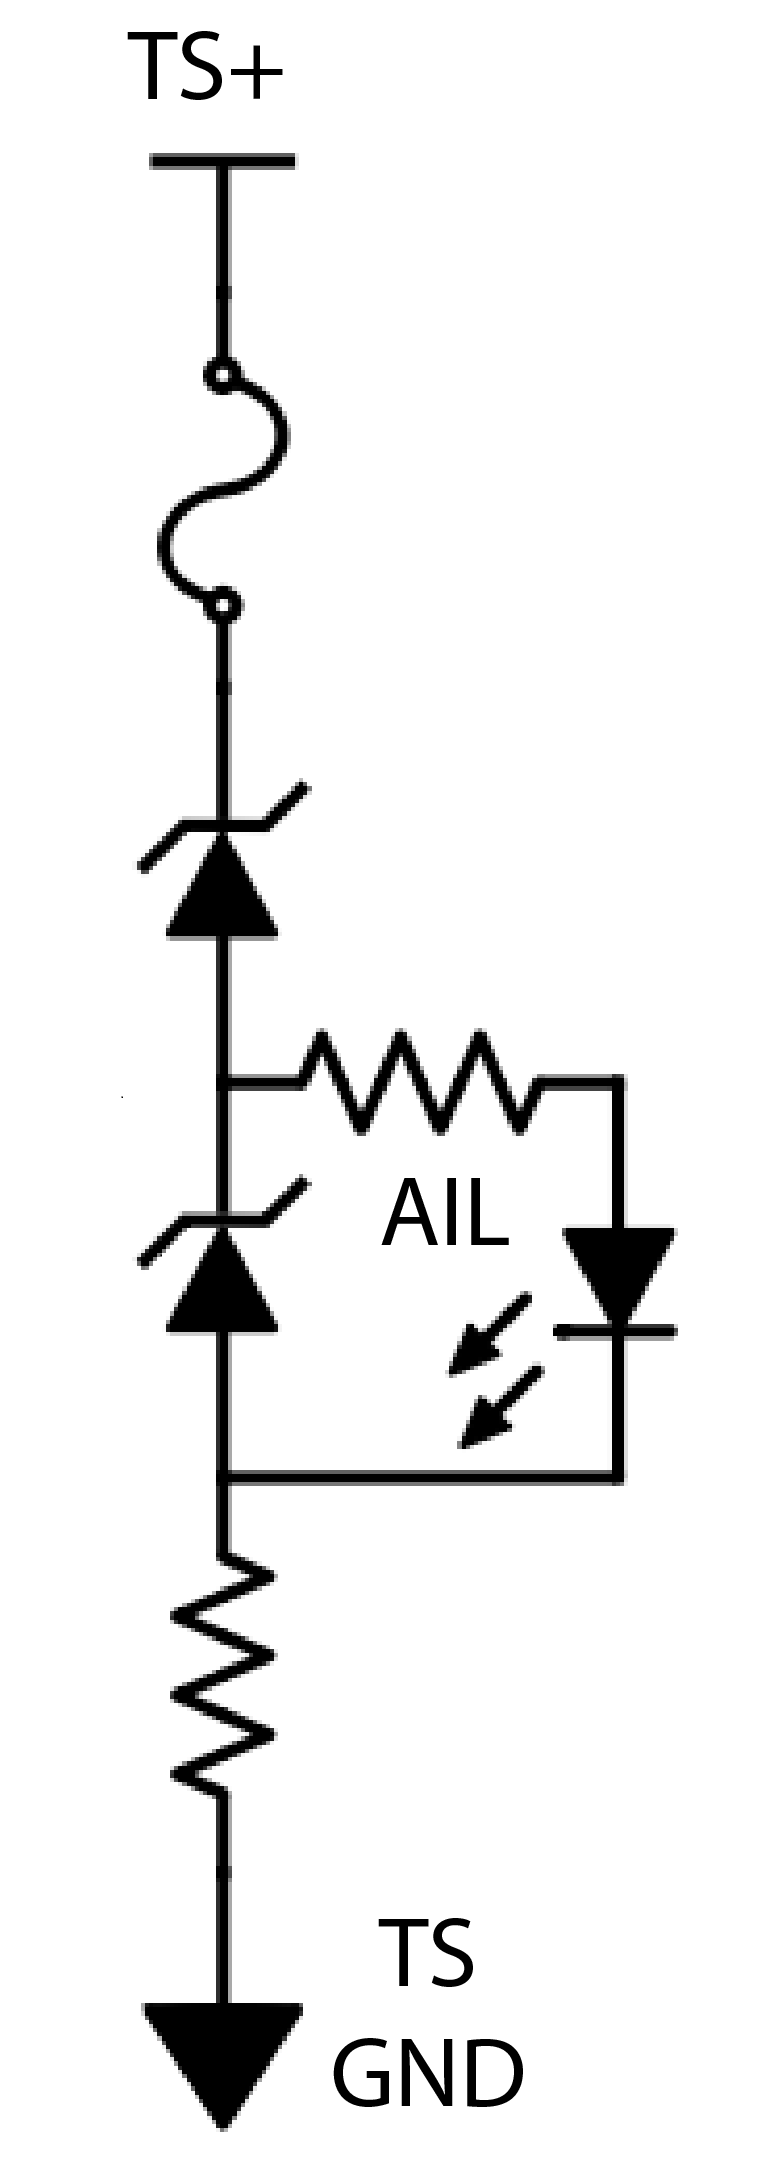
\includegraphics[scale=.8]{AIL.png}
\caption{Schematic for the AIL}
\label{fig:AILcircuit}
\end{figure}

The AIL will be located on the \hl{pre-charge} PCB, fused to \hl{3.15A}, and have traces of \hl{25} mil. All connections made by wires will be 20 AWG rated for 600V, 125°C and 7A.


\subsubsection{Wiring, cables, current calculations, connectors}\label{accumulator_wiring}
%Describe the internal wiring, show schematics, provide calculations for currents and voltages and show data regarding the cables and connectors used.
% Discuss maximum expected current, DC and AC how long will this be provided?
% Compare the maximum values to nominal currents
% Give a table for each kind of wire in your tractive-system:
% Describe your maintenance plugs, provide pictures
% Use tables like the one shown below:

%TODO

This wire is used for high power connections in the accumulator. High power connectors are documented in section \ref{shutdown_system_interlocks}. 

\begin{table}[H]
    \centering
    \begin{tabular}{|l|l|}
    \hline
    Wire type & \hl{2 AWG shielded cable}\\ \hline
    Current rating & \hl{255 A} \\ \hline
    Maximum operating voltage & 1 kV \\ \hline
    Temperature rating & -55\degree C to 150\degree C \\ \hline
    \end{tabular}
    \caption{Wire data of the company: Champlain Cable, \hl{EXRAD SAE 150 XLE Shielded Cable}}
    \label{accumulator_motortomcwire}
\end{table}



\subsubsection{Accumulator Insulation Relays (AIRs)}
%Describe the AIRs used and their main operation parameters, use tables, etc.
We will use KILOVAC EV200 contactors as our insulation relays. In compliance with EV3.3.5 they are mounted in a compartment separated from the rest of the accumulator by insulating G10/FR4 fiberglass. 

%talk about positioning inside the accumulator

	\begin{table}[H]
	    \centering
	    \begin{tabular}{|l|l|}
	        \hline
	        Relay Type: & Normally Open \\ \hline
	        Contact arrangement & SPST-NO-DM \\ \hline
	        Continuous DC current rating & 500A \\ \hline
	        Overload DC current rating & 2000A at 320VDC\\ \hline
	        Maximum operation voltage & 900VDC \\ \hline
	        Nominal coil voltage & 12VDC \\ \hline
	        Normal Load switching & Make and break up to 650A \\ \hline
	        Maximum Load switching & 3 times at 2,000A \\ \hline
	    \end{tabular}
	    \caption{Basic AIR Data}
	    \label{air}
	\end{table}

\subsubsection{Fusing}\label{accumulator_fusing}
%Describe the fuses used and their main operation parameters, use tables, etc.
%Additionally, fill out the following table for each fuse type used:
%TODO

	\begin{table}[H]
	    \centering
	    \begin{tabular}{|l|l|}
	    \hline
	        Fuse manufacturer and type: & \begin{tabular}[c]{@{}l@{}}Bussmann,\\ LPJ type\end{tabular} \\ \hline
	        Continuous current rating & \hl{200 A} \\ \hline
	        Maximum operating voltage & 600 V \\ \hline
	        Type of fuse & Time delay \\ \hline
	        I2t rating & Not Listed \\ \hline
	        \begin{tabular}[c]{@{}l@{}}Interrupt Current (max. current\\ at which the fuse can interrupt\\ the circuit)\end{tabular} & 300 kA \\ \hline
	    \end{tabular}
	    \caption{Tractive system main fuse, LPJ type. \href{http://www.cooperindustries.com/content/dam/public/bussmann/Electrical/Resources/product-datasheets-b/Bus_Ele_DS_1007_LPJ_70-600.pdf}{Datasheet here.}}
	    \label{tsfuse}
	\end{table}

%Create a table with components and wires protected by the fuse(s) and the according continuous current rating, below is an example table with some potential entries.  Complete this table with information for your design and add/remove additional locations as applicable.  Ensure that the rating of all the components is greater than the rating of the fuse such that none of the other components become the fuse.


    \begin{table}[H]
        \centering
        \begin{tabular}{|l|l|l|l|l|}
            \hline
            Location & Wire Size & Wire Ampacity & Fuse type & Fuse rating \\ \hline
            \begin{tabular}[c]{@{}l@{}}

            \hl{TS Main fuse (before HVD,\\ on pos pole)}\end{tabular} & \hl{2 AWG} & \hl{255A} & \hl{LPJ type} & \hl{200A} \\ \hline
            \begin{tabular}[c]{@{}l@{}}\hl{TS+ to IMD}\end{tabular} & \hl{22 AWG} & \hl{5A} & \hl{Littelfuse 808} & \hl{3.15A} \\ \hline
            \hl{Cell to BMS x72} & \begin{tabular}[c]{@{}l@{}}\hl{22AWG}\end{tabular} & \begin{tabular}[c]{@{}l@{}}\end{tabular} & \begin{tabular}[c]{@{}l@{}}\hl{PTC chip\\fuse x72}\end{tabular} & \hl{200mA }\\ \hline
        \end{tabular}
        \caption{\hl{Fuse Protection Table}}
        \label{allfuses}
    \end{table}

\hl{The Littelfuse 808 protecting the IMD is identical to the Littelfuse 80813150440 that protects the Vicor DC/DC converter. The datasheet can be found in appendix section {\ref{appendix_energy_meter_mounting}}. The PTC fuses datasheet can be found in appendix section {\ref{appendix_accumulator_fusing}}. }

\subsubsection{Charging}\label{accumulator_charging}
%Describe how the accumulator will be charged. How will the charger be connected? How will the accumulator be supervised during charging? Show schematics, CAD-Renderings, etc., if needed
%TODO

	\begin{table}[H]
	    \centering
	    \begin{tabular}{|l|l|}
	        \hline
	        Charger Type: & ELCON PFC 2000+ TCCH-288-6  \\ \hline
	        Maximum charging power & 24.9 A \\ \hline
	        Maximum charging voltage & 4.15 V (Per Cell) 298.8 V (Overall) \\ \hline
	        Maximum charging current & 5 A \\ \hline
	        Interface with accumulator & TE Connectivity HVP 800 lever action locking connector \\ \hline
	        Input voltage & 125VAC or 230VAC \\ \hline
	        Input current & 15A @ 125VAC or 8A @ 230VAC  \\ \hline
	    \end{tabular}
	    \caption{General Charger data}
	    \label{charger}
	\end{table}


 	\begin{figure}[H]
		\centering
		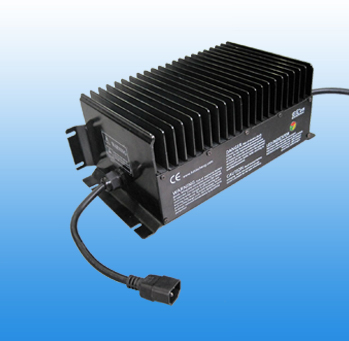
\includegraphics[width = 0.4 \textwidth]{Battery_Charger.jpg}
		\caption{Elcon PFC 2000+ Battery Charger}
		\label{Elcon Battery Charger}
	\end{figure}

	The charging system consists of two main components:  A charger that connects to the main pack connector and supplies the current needed to charge the accumulator, and a charging circuit that provides power to the AMS, opens the AIRS if the shutdown button is pressed, and displays critical information while charging. \hl{The IMD will remain active while the accumulator is charging.}
	
	This CE-Listed charger supplies constant current at 6A until cell voltages reach 4.15V. Then, constant voltage is supplied at 4.15V per cell, summing to 298.8 volts, until the cells are fully charged. The charging power lines are protected via the charger's short-circuit protection, which automatically stops charging if a short-circuit condition occurs.
	
	The charger interfaces with the accumulator through a lever action locking connector from TE Connectivity's HVP 800 series (P/Ns 2141227(accumulator side) and 2141154(charger side)). \hl{These connectors are connected to the charger by 10AWG wires through a charging interlock system that piggy-backs off of the discharge circuit, seen below in }\fref{fig:ChargerInterlock}.


	 \begin{figure}[H]
		\centering
		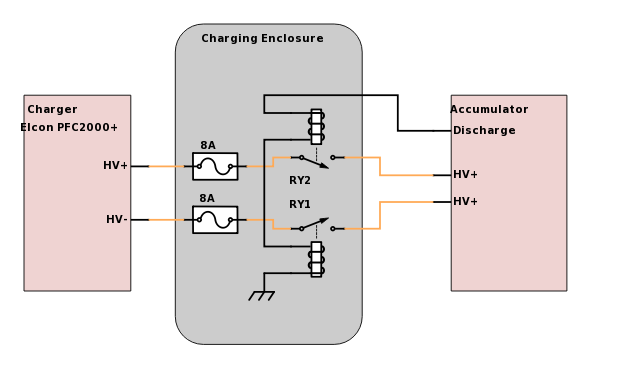
\includegraphics[width = 0.7 \textwidth]{Charging-Interlock.png}
		\caption{\hl{The charging interlock system, showing fuses and relays for charging the accumulator}}
		\label{fig:ChargerInterlock}
	\end{figure}
	
    \hl{The charging interlock system consists of two Littelfuse KLKD 10x38 600VDC 8A fuses connected to two Omron G9EJ-1-E 400VDC relays that are powered by the discharge circuit (the end of the accumulator shutdown circuit) mounted inside a protective enclosure on the charging cart. They only allow the charging connector to be energized if the shutdown circuit on the charging cart is closed meaning all of the HV and LV connectors are properly connected. See appendix section {\ref{appendix_accumulator_charger}} for datasheets.}
 	
	The accumulator will only be charged on the charging cart. The cart will be able to support the full weight of the accumulator and only move when a dead man's switch is activated.
	
	The accumulator cart will contain a specialized charging circuit that allows the accumulator to be charged through the main pack connector. The charging circuit mimics the shutdown circuit in the vehicle.The charging circuit will contain a clearly labeled emergency stop push button with a minimum diameter of 25mm which opens the AIRS and the charging relays ands stops charging. It will also communicate with the AMS over CAN and display critical information during charging.
	
	The AMS will be active during charging and have the ability to open the AIRS and stop charging in the event of dangerous battery conditions.The AMS will communicate with the Charger over CAN and turn off the charger in the event of a fault to maintain compliance with EV8.3.5. 
	
	

\subsubsection{Mechanical Configuration/materials}\label{accumulator_mechanical_configuration}
%Describe the concept of the container, show how the cells are mounted, use CAD-Renderings, show data regarding materials used, etc.


\hl{The main structure of the accumulator container is made from .050" 430 stainless steel sheet. The front, left, right, and bottom walls are made from one folded sheet. The rear wall is made from another folded sheet. Inside are six segments of 12 cells. The segments are separated by internal vertical walls. The internal vertical walls are made from 20ga (.0359") 430 stainless steel sheet. The internal vertical walls are attached to the bottom wall with spot welds. The internal vertical walls are attached to the external vertical walls with spot welds. All walls are internally lined with a sheet of garolite to provide insulation.}

\begin{figure}[H]
\centering
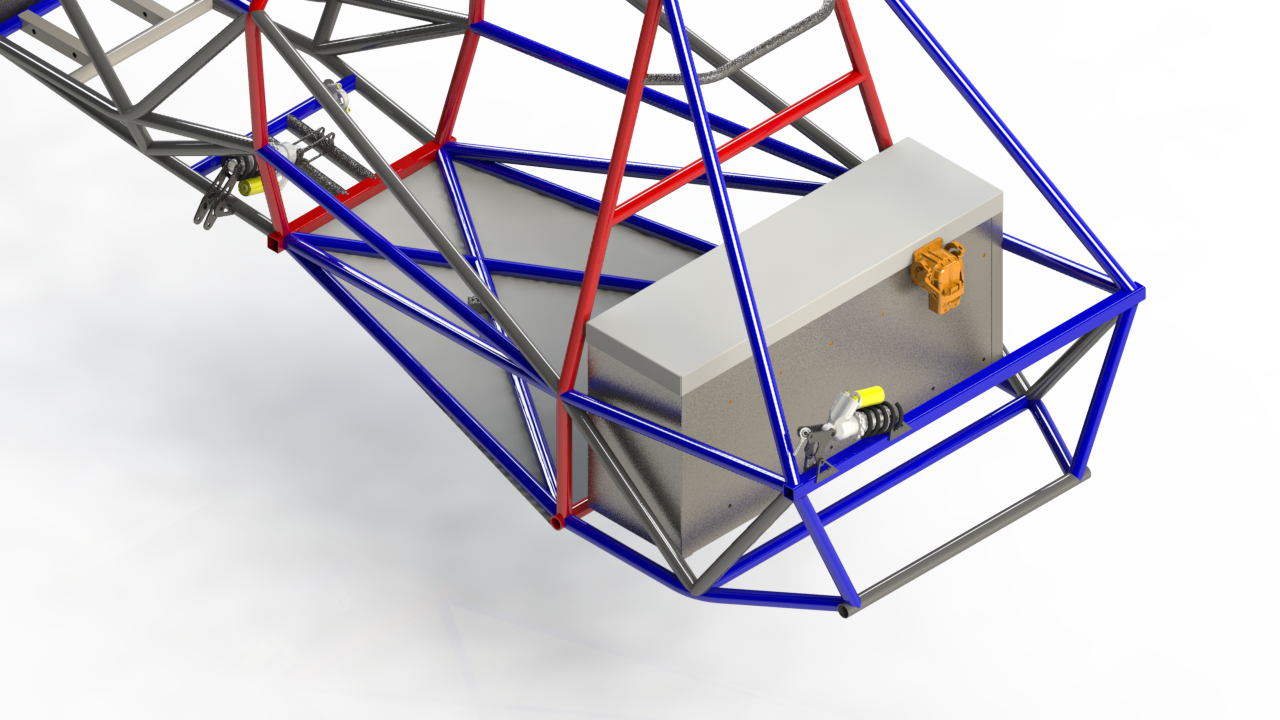
\includegraphics[width=1\textwidth]{accumulator}
\caption{\hl{Isometric render of the fully assembled accumulator. }}
\label{fig:accumulator}
\end{figure}

\hl{The cells we are using must be compressed on their large face to within the manufacturer recommended range (4-18psi). We are considering two methods of cell compression. In the first, the cells are compressed between  two aluminum face sheets by threaded rods. 4 threaded rods are used to compress each segment. In the second method, the threaded rods are replaced by aluminum end caps that set the distance between the aluminum face sheets. In both methods, cell compression pressure will be set by imposing a strain on the stack. The materials will be characterized and the necessary strain will be applied such that the cells remain in the specified pressure range. Each compressed segment is individually installed into the accumulator, then the rear wall is attached.}

\begin{figure}[H]
\centering
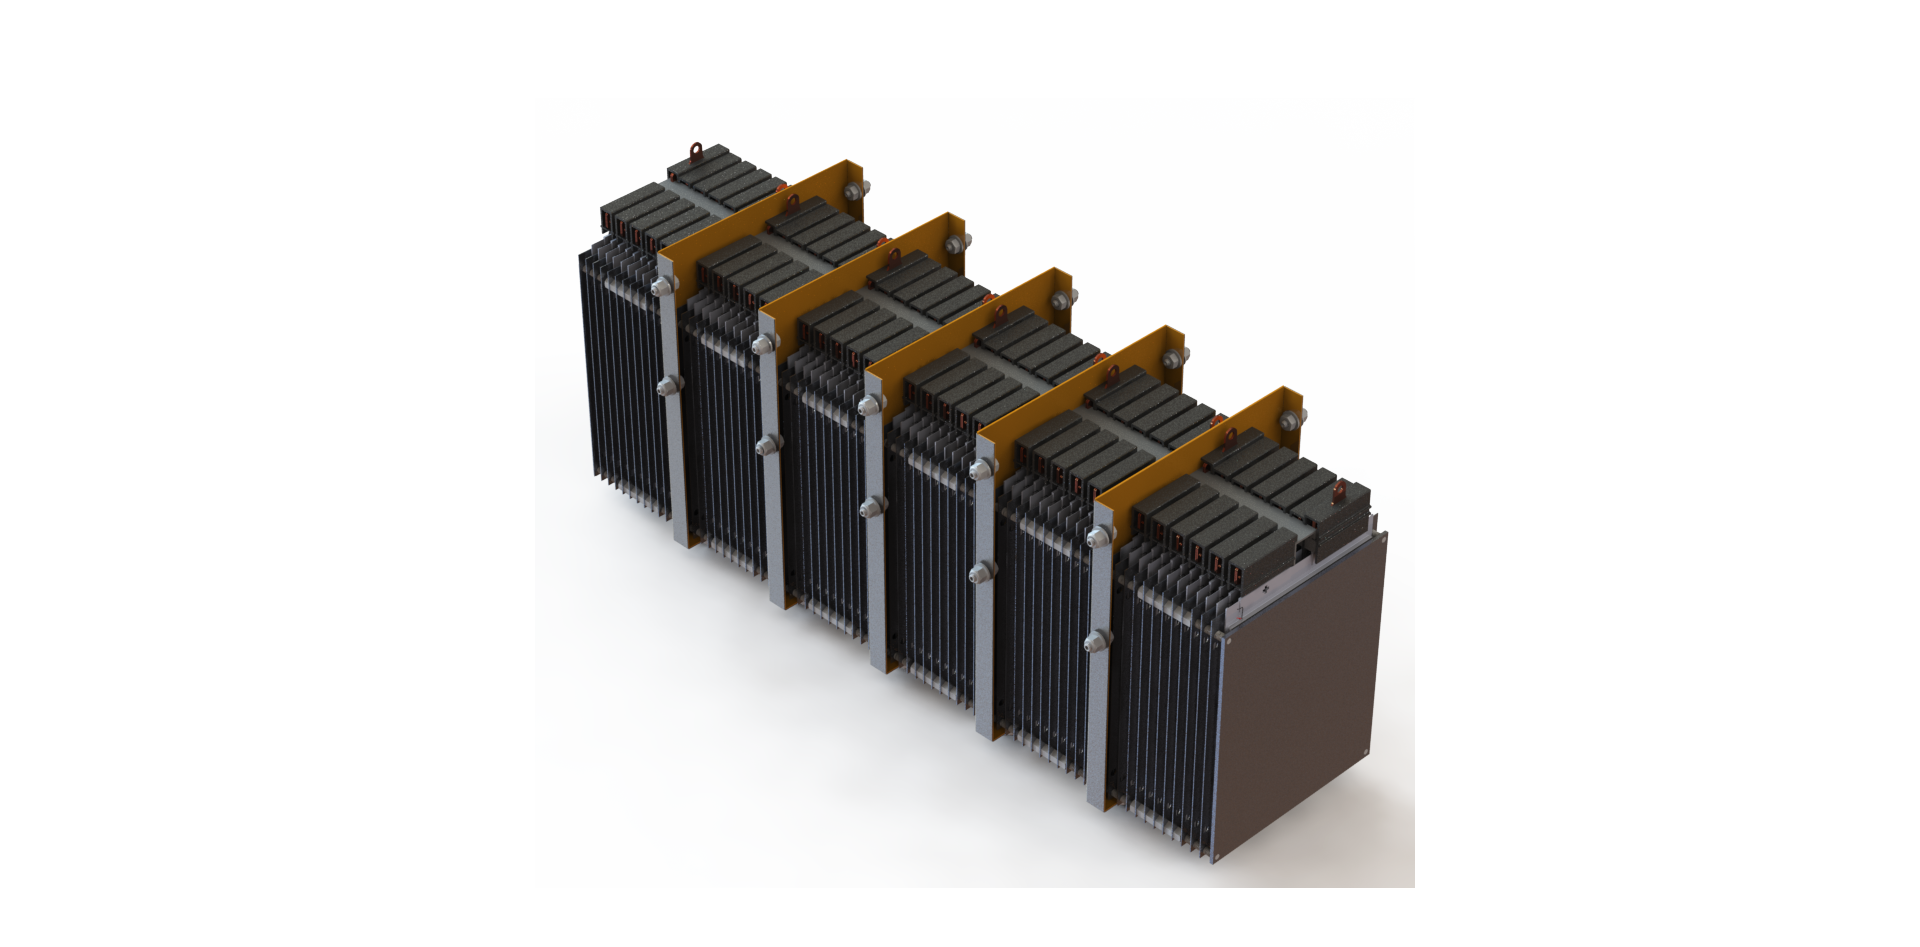
\includegraphics[width=1\textwidth]{cell_stack}
\caption{Configuration of cell modules, with dividing walls.}
\label{fig:cell_stack}
\end{figure}


\hl{Individual cells are connected by squeezing their tabs together with bolted copper plates. Voltage sensing is done using wires connected to these plates. Each bolted plate assembly is isolated with a 3d-printed cover. This cover protects each terminal from shorts during assembly and maintenance. Each cover is retained with a zip-tie. Thermistors are epoxied to the negative terminal of all cells for temperature monitoring.

The Accumulator Interrupt Relays, Main Pack Fuse, Battery Management System, Service Disconnects, and other related electronics are located in the top section of the accumulator. This section is separated from the lower section by a .050" 430 stainless sheet that is insulated on both sides by 1/32" garolite. The divider is fastened with 18 1/4"-20 grade 5 fasteners. The top section is closed with a lid similar to the divider. It is attached to the side walls with an identical fastener pattern.

All structural fasteners are secured with nylok nuts. The nylok nuts are all located outside the accumulator container. All insulating garolite is epoxied to the surface it insulates.}


\subsubsection{Position in car}
%Provide CAD-renderings showing the relevant parts. Mark the parts in the rendering, if necessary.  Ensure that the required mechanical structure to protect the accumulator and other electrical components is clearly identified.

\begin{figure}[H]
	\centering  % this centers the image
	
	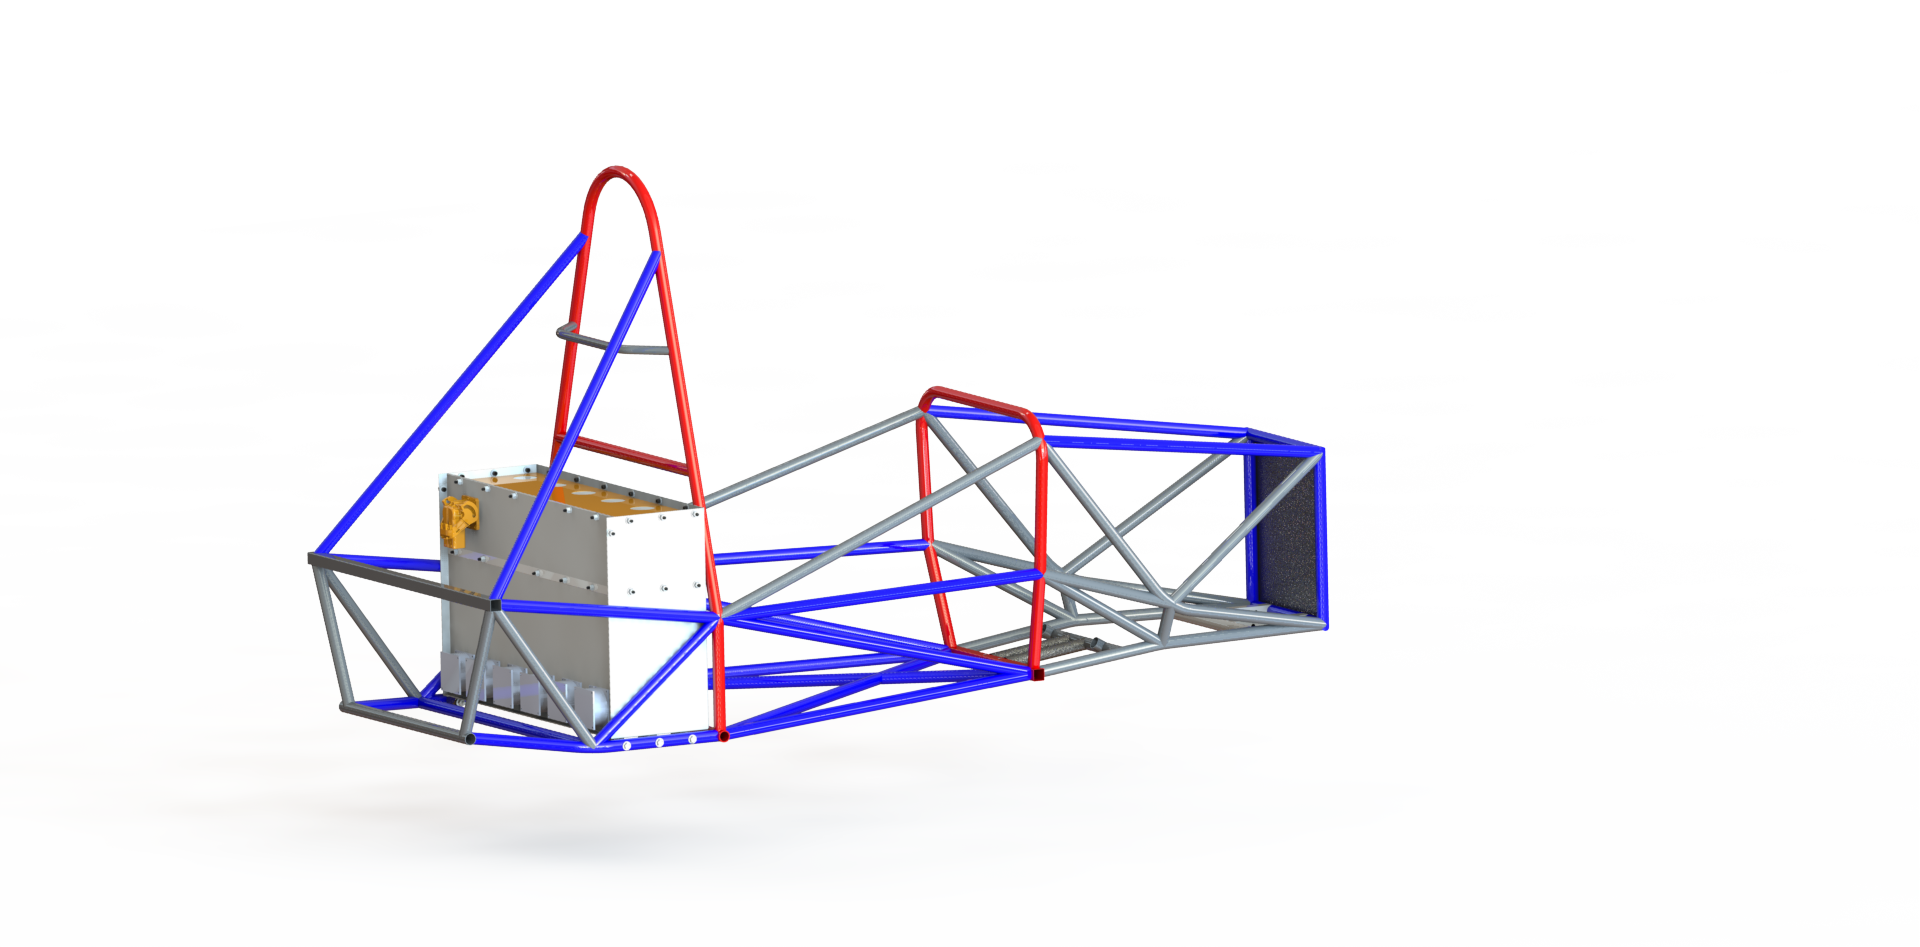
\includegraphics[width=1\textwidth]{acc_in_frame}
    %\captionsetup{margin={0.3\textwidth,0.3\textwidth}}
	
	\caption{\hl{Position of the accumulator in the frame.}}
	
	\label{fig:acc_in_frame}
\end{figure}

\subsection{Accumulator pack 2}\label{accumulator_pack_2}
We only have one accumulator, described in \ref{accumulator_pack_1}.

\section{Energy meter mounting} \label{energy_meter_mounting}
\subsection{Description}
%Describe where the energy meter is mounted and how, etc.
The vehicle's energy meter is mounted in a dedicated tractive system enclosure at the rear of the car that we call the energy meter enclosure. As is visible in \fref{fig:TS_block_diagram}, the energy meter enclosure is a pass-through enclosure that connects in series with both poles of the tractive system between the accumulator and the motor controller. Inside are the energy meter, the high-voltage low-current fuses that protect the TSAL (section \ref{tractive_system_active_light}), the current-limiting resistors that protect the TSMPs (section \ref{measurement_points}), and the discharge circuit (section \ref{discharge_circuitry}). 

\subsection{Wiring, cables, current calculations, connectors}
%Describe the wiring, show schematics, provide calculations for currents and voltages, and show data regarding the cables and connectors used.

The energy meter current calculations require it to be connected in series with the low pole of the tractive system. It is bolted onto custom-made copper bus bars with \hlr{serrated, distorted-thread locking }fasteners to ensure electrical connection, \hlr{which can be seen in }\fref{fig:energy_meter_internals}. 

\begin{figure}[H]
\centering
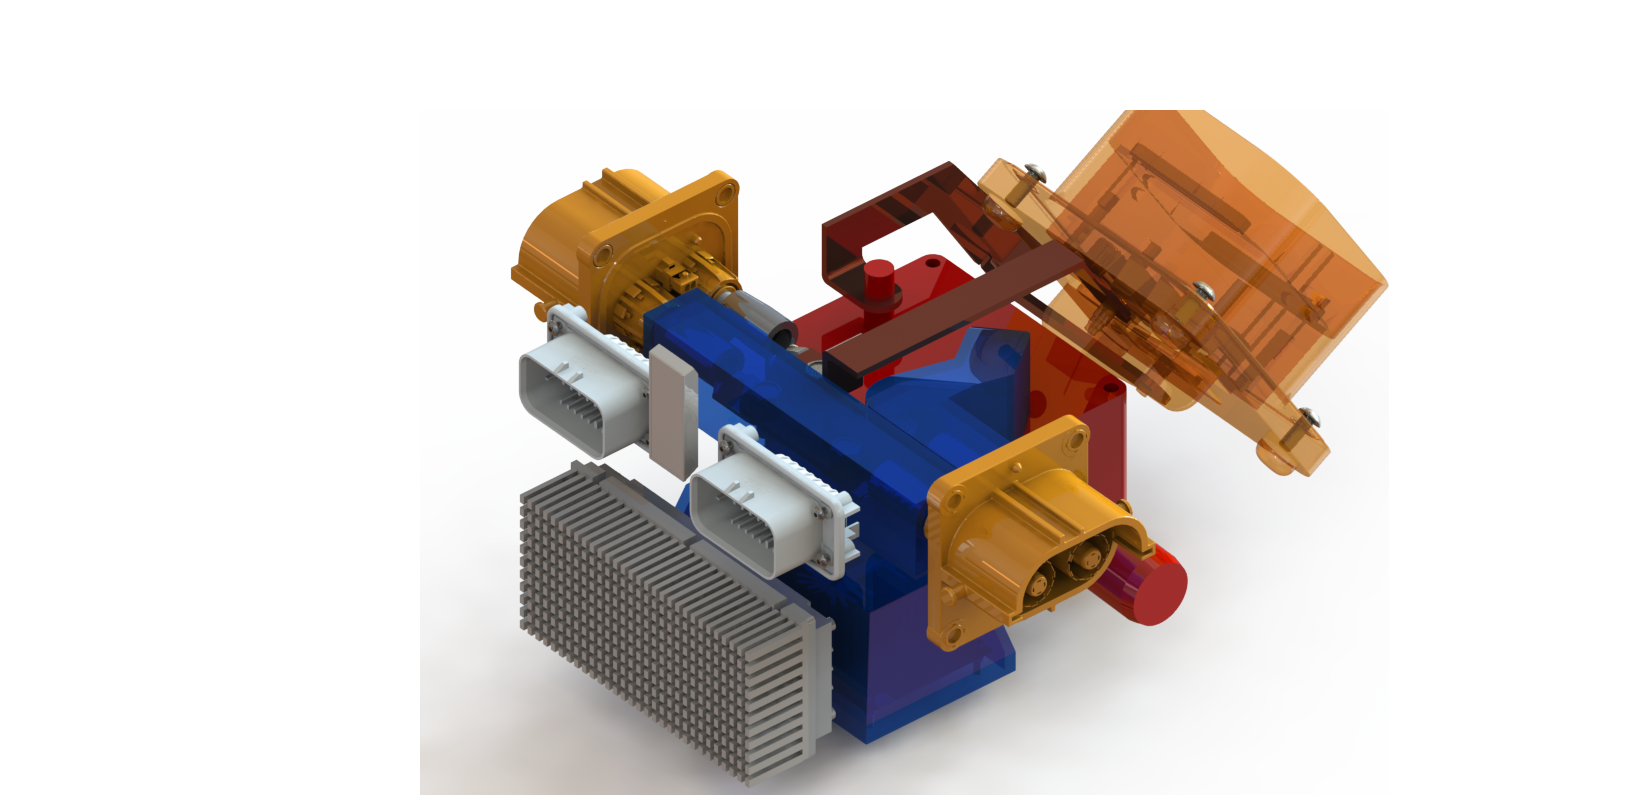
\includegraphics[width=0.8\textwidth]{EnergyMeterExposedInternalsCovered}
\caption{\hlr{Rendering of the internal geometry of the energy meter enclosure. The energy meter itself is visible in red. The blue solids are insulating covers to separate the individual HV bus bars from one another and to protect the LV energy meter circuitry at the base of the enclosure. See }\fref{fig:energy_meter_mounting_render}\hlr{ for a render of the enclosure in the vehicle}}
\label{fig:energy_meter_internals}
\end{figure}

\Fref{fig:energy_meter_internals_enclosure} \hlr{shows the internals of the energy meter enclosure from another angle, also including the housing. Internal covers are removed to show bus bar geometry. Bus bars will be wrapped in Kapton polyimide tape with a protective heat-shrink sleeve.}

\begin{figure}[H]
\centering
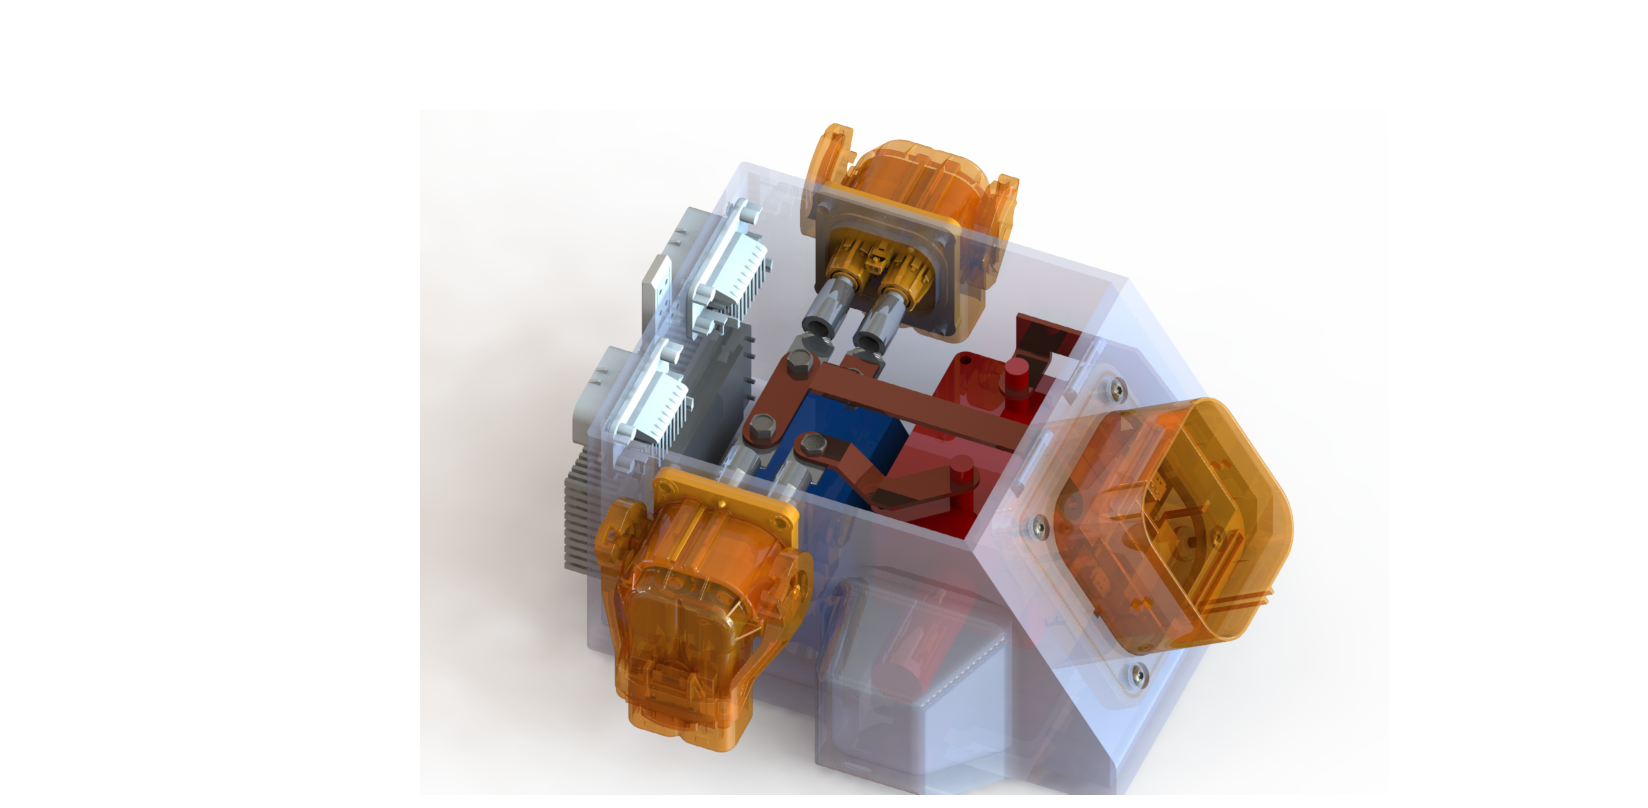
\includegraphics[width=0.8\textwidth]{EnergyMeterInternalsNoCovers}
\caption{\hlr{Rendering of the energy meter enclosure showing the housing. Internal bus bar covers have been hidden to show bus bar structure.}}
\label{fig:energy_meter_internals_enclosure}
\end{figure}

Voltage measurement connections to TS+ for the energy meter, and connections for the TSAL fuses and TSMP current-limiting resistors are made via ring terminals to the corresponding bus bars. The wires for the TSMPs, the TSAL, and the energy meter will all be 20AWG rated to 300V and 90\textdegree C. The energy meter itself also requires GLVS power, which means that proper HV wire spacing of 30mm will be upheld. 



\begin{figure}[H]
\centering
\includegraphics[width=0.6\textwidth]{Energy-Meter-Schematic-w-HVD.png}
\caption{Schematic of the internals of the energy meter. Fuses S1 and S2 are Littelfuse 80813150440s, and resistors R1 and R2 are the TSMP resistors from section \ref{measurement_points}.}
\label{fig:energy_meter_schematic}
\end{figure}

\Fref{fig:energy_meter_schematic} shows the internals of the energy meter box \hlr{in electrical schematic form}. The GLVS connector contains the shutdown circuit power for the discharge circuit, the interlock from the HVD, and GLVS power for the energy meter. The high voltage low power connector contains TSMP and TSAL high voltage connections to the master switch panel. High power connections are shown in orange.

The energy meter TS+ connection and the TSAL TS+ measurement wire share the same fused connection, and the TSAL TS- measurement wire has its own fuse. The fuse specifications can be found in \fref{tab:TSAL_and_EM_fuse}. The datasheet for the fuse can be found in \fref{tab:TSAL_and_EM_fuse}.

\begin{table}[H]
	\centering
	\begin{tabular}{|l|l|}
	\hline
	Fuse manufacturer and type & Littelfuse 80813150440 \\ \hline
	Continuous current rating & 2.00 A \\ \hline
	Maximum operating voltage & 450VDC \\ \hline
	Type of fuse & Fast-acting \\ \hline
	I2T & 0.0610 A$^{2}$sec \\ \hline
	Interrupt current rating & 10,000 A \\ \hline
	\end{tabular}
	\caption{TS+ fuse for energy meter and TSAL TS+ measurement wire}
	\label{tab:TSAL_and_EM_fuse}
\end{table}

\subsection{Position in car}
%Provide CAD-renderings showing all relevant parts. Mark the parts in the rendering, if necessary.
The energy meter housing is mounted to the chassis at the rear of the vehicle, in close proximity to the motor, motor controller, and accumulator, and with the HVD easily visible and accessible from the rear. See \fref{fig:energy_meter_mounting_render}.

\begin{figure}
\centering
\includegraphics[width=0.5\textwidth]{EnergyMeterBackISO}
\caption{Render of the rear of the vehicle showing the mounting for the energy meter enclosure at the rear of the vehicle}
\label{fig:energy_meter_mounting_render}
\end{figure}


\section{Motor controller}\label{motor_controller}
\subsection{Motor controller 1}\label{motor_controller_1}
\subsubsection{Description, type, operation parameters}
%Describe important functions; provide table with main parameters like resulting voltages->minimum, maximum, nominal, currents etc.

The motor controller regulates the power delivered to the motor. This motor controller is preferable for its small package and isolated control interface. We will communicate with it using our CAN bus. 

\begin{table}[H]
	\centering
	\begin{tabular}{|l|l|}
	\hline
	Motor Controller type & Rinehart PM100DX \\ \hline
	Maximum continuous power & 86 kVA \\ \hline
	Maximum peak power & 100 kVA for 10s \\ \hline
	Maximum input voltage & 400 VDC \\ \hline
	Output voltage & Not listed \\ \hline
	Maximum continuous output current & 300 A \\ \hline
	Maximum peak current & 350 A for 10s \\ \hline
	Control method & CAN \\ \hline
	Cooling method & Water \\ \hline   
	Auxiliary supply voltage & 12 VDC \\ \hline
	\end{tabular}
	\caption{General Motor Controller data}
	\label{MC}
\end{table}

\subsubsection{Wiring, cables, current calculations, connectors}
%Describe the wiring, show schematics, provide calculations for currents and voltages and show data regarding the cables and connectors used.

The PM100DX has five high voltage connections (DC+, DC-, Phase A, Phase B, Phase C) as seen in \fref{fig:TS_block_diagram}. Each connection is done with a cable gland that provides strain relief, environmental sealing, and shield termination for the dual insulated shielded 4 AWG cable. The manufacturer recommends this particular cable from Champlain Cable. 

\begin{table}[H]
	\centering
	\begin{tabular}{|l|l|}
	\hline
	Wire type & 4 AWG Cable\\ \hline
	Current rating & 190 A \\ \hline
	Maximum operating voltage & 1 kV \\ \hline
	Temperature rating & -55\degree C to 150\degree C \\ \hline
	\end{tabular}
	\caption{Wire data of the company: Champlain Cable, EXRAD SAE 150 XLE Shielded Cable}
	\label{motor_controller_motortomcwire}
\end{table}

\subsubsection{Position in car}
%Provide CAD-renderings showing the relevant parts. Mark the parts in the rendering, if necessary.
\begin{figure}[H]
    \centering
    \includegraphics[scale=1]{MotorController3-1-17.png}
    \caption{CAD rendering of Motor Controller position}
    \label{mc_cad}
\end{figure}

\subsection{Motor controller 2}
We only have one motor controller, described in \ref{motor_controller_1}.

\section{Motors}\label{motors}
\subsection{Motor 1}\label{motor_1}

\subsubsection{Description, type, operating parameters}
%Describe the motor used, provide table with main parameters like resulting voltages->minimum, maximum, nominal, currents, resulting motor power, use figures to show important characteristics.
Originally designed for aviation use, this out-runner motor delivers remarkable performance for its weight. 

\begin{table}[H]
	\centering
	\begin{tabular}{|l|l|}
	\hline
	Motor Manufacturer and Type: & \begin{tabular}[c]{@{}l@{}}Make: Enstroj \\ Model: EMRAX 228\end{tabular} \\ \hline
	Motor principle & Permanent magnet synchronous motor \\ \hline
	Maximum continuous power & 28 - 42 kW \\ \hline
	Peak Power & 100 kW \\ \hline
	Input voltage & 50 – 450 V \\ \hline
	Nominal current & 160 A \\ \hline
	Peak current & 340 A \\ \hline
	Maximum torque & 240 Nm \\ \hline
	Nominal torque & 125 Nm \\ \hline
	Cooling method & Water \\ \hline
	\end{tabular}
	\caption{General motor data}
	\label{motortable}
\end{table}

% Give a plot of power vs. Rpm including a line for nominal and maximum power
% Give a plot of torque vs. rpm including a line for nominal and maximum torque

\begin{figure}[H]
    \centering
    \includegraphics[width = 1 \textwidth]{motor_power_torque.jpg}
    \caption{Motor Power and Torque: although we are using the medium voltage version of the motor, the only difference in terms of this plot is the ratio of current and voltage. }
    \label{motor_power_torque}
\end{figure}


\subsubsection{Wiring, cables, current calculations, connectors}
%Describe the wiring, show schematics, provide calculations for currents and voltages and show data regarding the cables and connectors used.
\begin{table}[H]
    \centering
    \begin{tabular}{|l|l|}
    \hline
    Wire type & 2 AWG Cable\\ \hline
    Current rating & 255 A \\ \hline
    Maximum operating voltage & 1 kV \\ \hline
    Temperature rating & -55\degree C to 150\degree C \\ \hline
    \end{tabular}
    \caption{Wire data of the company: Champlain Cable, EXRAD SAE 150 XLE Shielded Cable. \href{http://www.champcable.com/wp-content/uploads/2016/08/SAE-EXRAD-150-HVFX-Shielded-XLE-150Jacketed-Battery-Cable-1.pdf}{Datasheet here}}
    \label{motor_motortomcwire}
\end{table}

Since the motor leads terminate close to the motor with ring terminals close to the motor as seen in figure \ref{motor_pic}, the motor will have a 3D printed enclosure around the leads, with a high power connector found \href{http://www.te.com/usa-en/product-2141230-2.html}{here.} \hlr{A CAD render of the motor lead enclosure can be found in }\fref{fig:motor_enclosure}. \hlr{HV and LV segments are separated by a 3D printed wall with an extension designed to protect the LV rotary encoder wires from the motor from HV connections. HV connections will be shielded and double-insulated, so the plastic serves to keep the wires from interfering, not to provide insulation.}

\begin{figure}[H]
    \centering
    \includegraphics[width = 0.8 \textwidth]{MotorBoxAssemblyRender2}
    \caption{\hlr{CAD render of 3D printed motor enclosure. HV and LV segments of the enclosure are separated by a PLA wall.}}
    \label{fig:motor_enclosure}
\end{figure}

\begin{figure}[H]
    \centering
    \includegraphics[width = 0.6 \textwidth]{motor_pic}
    \caption{Picture of motor, note ring terminal crimps on leads. }
    \label{motor_pic}
\end{figure}

\subsubsection{Position in car}
%Provide CAD-renderings showing all relevant parts. Mark the parts in the rendering, if necessary and clearly identify the structure used to protect all relevant parts.

\begin{figure}[H]
    \centering
    \includegraphics[width = 0.8 \textwidth]{motor_side}
    \caption{CAD rendering of the motor and transmission in the frame of the vehicle}
    \label{motor_side}
\end{figure}

\begin{figure}[H]
    \centering
    \includegraphics[width = 0.8 \textwidth]{motor_rear}
    \caption{CAD rendering of the motor and transmission in the frame of the vehicle}
    \label{motor_rear}
\end{figure}

\begin{figure}[H]
    \centering
    \includegraphics[width = 0.8 \textwidth]{motor_iso}
    \caption{CAD rendering of the motor and transmission in the frame of the vehicle}
    \label{motor_iso}
\end{figure}

\begin{figure}[H]
    \centering
    \includegraphics[width = 0.8 \textwidth]{motor_dimetric}
    \caption{CAD rendering of the motor and transmission in the frame of the vehicle}
    \label{motor_dimetric}
\end{figure}

\subsection{Motor 2}\label{motor_2}
We only have one motor, described in \ref{motor_1}.

\section{Torque encoder}\label{torque_encoder}
\subsection{Description/additional circuitry}
%Describe the type of the torque encoder(s) used, provide tables with main operation parameters, and describe additional circuitry used to check or manipulate the signal going to the motor controller. Describe how the system reacts if an implausibility or error (e.g. short circuit or open circuit or equivalent) is detected.

Two \hl{hall-effect-based rotary encoders} are mechanically housed in one unit, \hl{the Magni-Tec MHR5261, which is} mounted to the rotating shaft of the throttle pedal assembly. The use of a single housing eliminates concerns regarding mechanical backlash and misalignment. \hl{See section {\ref{appendix_torque_encoder}} for datasheet.} Each output from \hl{the encoders} will \hl{be measured by a} CAN-connected ATmega16M1, which will compare the two outputs and send a message via CAN bus to the motor controllers with the requested torque.

\begin{table}[H]
	\centering
	\begin{tabular}{|l|l|}
	\hline
	Torque encoder manufacturer and type: & \hl{Magni-Tec MHR5621} \\ \hline
	Torque encoder principle & \hl{Hall-effect-based voltage source} \\ \hline
	Supply voltage & 5V \\ \hline
	Maximum supply current & 15 mA \\ \hline
	Operating temperature & -55 to 150\degree C \\ \hline
	Used output & 0-5V \\ \hline
	\end{tabular}
	\caption{Torque Encoder data}
	\label{encoder}
\end{table}

\subsection{Torque Encoder Plausibility Check}\label{torque_encoder_plausibility_check}
%Describe additional circuitry used to check or manipulate the signal going to the motor controller. Describe how failures (e.g. Implausibility, short circuit or open circuit or equivalent) are detected and how the system reacts if an implausibility or errors is detected.

Two \hl{rotary encoders} are mounted on the torque pedal. A CAN node probes the voltage dividers which are amplified in different transfer functions using a Texas Instruments Operational Amplifier, part number LMV341QDCKRQ1. One \hl{op-amp} amplifies the voltage of one \hl{encoder} by a factor of two and the other amplifies the voltage from the \hl{other encoder} by a factor of one half. The ATmega will compare the two independent voltages and if an implausibility occurs, a difference in voltage from the Torque Encoder besides what is expected from the transfer function, and persists for more than 100msec, the power to the motor(s) must be immediately shut down completely. If a short circuit or wiring failure with either potentiometer occurs, the input will be outside the normal operating range, and the power to the motor controllers will be shut down. \hlr{The normal operating range for the throttle inputs will be from 0.5V to 4.5V on the analog line with a gain of 2, and from 2 to 3 volts on the analog line with a gain of 1/2. Upon detecting an implausibility, the ATmega16m1 ADC will trigger an interrupt that the input voltage is outside the defined range, and a software timer will begin. If the software timer reaches 100 msec before the input voltage triggers a "return to normal range" interrupt, then the APPS will trigger a motor shutdown over CAN.} The node will log the error in the CAN bus. There will also be a Pegasus Brake light pressure switch (part number 3601, recommended by Formula Hybrid) on the brakes, wired to a CAN node with 22 gauge wire. If the pressure switch indicates actuation of the brake and the \hlr{accelerator pedal position sensor} measures more than 25 percent pedal travel, the power to the motors will be completely stopped until the accelerator pedal indicates less than 5 percent pedal travel. 

\hl{In addition to the torque encoder plausibility check in the ATmega software, we also implement a CAN message timeout in the motor controller for stale throttle signals. If the motor does not receive a CAN message from the throttle CAN node for 300 ms (a parameter in the motor controller configuration) it will stop power to the motors. See appendix section {\ref{appendix_torque_encoder}} for PM100DX motor controller datasheet excerpt.} 

\subsection{Wiring}
%Describe the wiring, show schematics, show data regarding the cables and connectors used.

Two potentiometers are wired with their each input wired through an operational amplifier with a specific amplification, one with an amplification of two and one with an amplification of one half, and their output to the CAN analog input pins. The potentiometers are given separate power lines of 5V, parallel, to the supply power of the CAN node itself. The brake switch is positioned to trip at a level of hard braking, and when triggered will deliver 5V to a CAN input pin. The CAN node is wired to send and receive messages to the other nodes.

\subsection{Position in car/mechanical fastening/mechanical connection}
%Provide CAD-renderings showing all relevant parts and discuss the mechanical connection of the sensors to the pedal assembly. Mark the parts in the rendering, if necessary.
The torque encoder is bolted to the accelerator pedal assembly with 4x ¼”-20 bolts. The bolts are safetywired to prevent loosening. The torque encoder is manufactured with a D-shaft. This is rotationally fixed to the accelerator pedal axle by a 4-40 set screw. The set screw is bonded with Loctite Purple to prevent loosening. This allows the torque encoder to measure the angular position of the accelerator pedal axle. The accelerator pedal axle is prevented from moving axially by retaining rings. The mounting of the torque encoder does not affect the relative plausibility check. The sensor used contains two independent encoders, each measuring the position of the single shaft 

\begin{figure}[H]
    \centering
    \includegraphics[width=\linewidth]{encoder_connection.png}
    \caption{Mechanical fastening and connection to the throttle pedal. Note that the torque encoders are two encoders housed in one package}
    \label{fig:encoder_position}
\end{figure}

\begin{figure}[H]
    \centering
    \includegraphics[width=\linewidth]{encoder_mount}
    \caption{Location of the encoder on the throttle pedal}
    \label{fig:encoder_mount}
\end{figure}

\begin{figure}[H]
    \centering
    \includegraphics[width=\linewidth]{encoder_car_location}
    \caption{Location of torque encoder in car} 
    \label{fig:encoder_car}
\end{figure}


\section{Additional LV-parts interfering with the tractive system}
\subsection{LV part 1}
%Describe those parts here which interfere or influence the tractive system, for example a controlling unit that measures wheel speeds and steering angle and calculates a target torque for each motor or a DC/DC-Converter providing power for the LV-system from the HV-system, etc.
There are preliminary design ideas for adding a DC/DC converter into the energy meter enclosure for recharging the GLVS battery, but that design has not yet been considered, and will only appear in a later revision of the ESF if it is included in the vehicle. As of yet all LV parts interfering with the tractive system have been adequately described in other sections.

\subsubsection{Description}
%Describe the parts used and their circuitry, and provide main operation parameters, use tables or figures, etc.
All LV parts interfering with the tractive system have been adequately described. 

\subsubsection*{Wiring, cables}
%Describe the wiring, show schematics, etc.
All LV parts interfering with the tractive system have been adequately described. 

\subsubsection{Position in car}
%Provide CAD-renderings showing the relevant parts. Mark the parts in the rendering, if necessary.
All LV parts interfering with the tractive system have been adequately described. 

\subsection{LV part 2}
All LV parts interfering with the tractive system have been adequately described. 

\section{Overall Grounding Concept}\label{overall_grounding_concept}
\subsection{Description of the Grounding Concept}
%Describe how you intend to achieve the resistances between components at the required levels as defined in EV4.3.
The vehicle's steel chassis is uses as GLVS ground. This ground will be established inside the master switch panel enclosure by attachment to a positively-retained ring terminal on a chassis member that has been locally stripped of paint. All components of the GLVS will be grounded to this point on the chassis through the wiring harness for simplicity of installation and mechanical robustness. All conductive mechanical enclosures are mounted to the chassis with conductive metal fasteners. Electrical connection of the suspension members and knuckles to the main vehicle frame will be achieved by short jumpers with ring terminals on either end in the suspension member bolt stackup on either side of the spherical bearing.


\subsection{Grounding Measurements}
%Describe which measurements you will take to ensure that EV4.3 is achieved
All conductive components within 100 mm of any Tractive System or GLVS component will be measured by Kelvin ohmmeter to have a resistance of less them 300 m$\omega$ to chassis ground, measured at the chassis ground measurement point on the master switch panel. All fastened mechanical components and enclosures will be individually measured to ensure proper ground connection. Chassis ground continuity will be tested during and after assembly to ensure complete coverage. Any carbon fiber components will be exhaustively measured to ensure resistance compliance.

\section{Firewall(s)}\label{firewalls}
\subsection{Firewall 1}\label{firewall_1}
\subsubsection{Description/materials}
%Describe the concept, layer structure and the materials used for the firewall. Show how the low resistance Control System ground connection is achieved.
The firewall is constructed of two layers. The layer facing the tractive system is 24 gauge Aluminum sheet metal, and the layer facing the cockpit is 24 gauge Flame-Retardant Multipurpose Garolite. The assembly is attached with marine epoxy between the two layers and nylon fasteners. The chassis has welded sheet metal tabs that fasten to the firewall with bolts and lock nuts. Because the firewall is fastened to the chassis using conductive fasteners it is connected to GLV ground. The firewall is attached to the seat through epoxied 3D printed spacers and foam sprayed between the seat and firewall, seen in \fref{fig:firewall_exploded}.
All high voltage and high temperature systems are contained in the rear of the vehicle, so only one firewall will be used. There are GLV systems in the dashboard and pedal box so a small grommet hole will be made in the firewall for GLV wiring.

\begin{figure}[H]
    \centering
    \includegraphics[width = 1 \textwidth]{firewall_exploded.png}
    \caption{An exploded view of the firewall and seat. }
    \label{fig:firewall_exploded}
\end{figure}

\subsubsection{Position in car}
%Provide CAD-renderings showing all relevant parts. Mark the parts in the rendering, if necessary.
The firewall is located between the driver and accumulator, to protect the driver from the tractive system. \fref{fig:firewall_in_car} shows the cockpit view without the seat for visual aid. The seat is between the wheel and the firewall, with the firewall cushioning the seat.  The firewall is attached to the frame so that its top corners are flush, eliminating a concern of sharp edges.

\begin{figure}[H]
    \centering
    \includegraphics[width = 1 \textwidth]{firewall_in_car.png}
    \caption{A view of the firewall in the car without the seat. }
    \label{fig:firewall_in_car}
\end{figure}

\subsection{Firewall 2}\label{firewall_2}
We only have one firewall, described in \ref{firewall_1}.


% Appendix starts here ------------------------------------------------------------------------------------------------------------------------------------

\section{Appendix}\label{appendix}
\setcounter{subsection}{1}
\subsection{Electrical Systems}\label{appendix_electrical_systems}
\setcounter{subsubsection}{1}
\subsubsection{IMD Datasheet}\label{IMD_datasheet}
\hlr{Referred from section} \ref{imd}.

\begin{figure} [H]
	\centering  % this centers the image
	
	\includegraphics[width=\textwidth]{Formula_IMD_Datasheet.png}
	\captionsetup{margin={0.3\textwidth,0.3\textwidth}}
	
	\caption{The datasheet for the IMD.}
	
	\label{fig:IMD_Datasheet}
\end{figure}

\href{http://www.bender-us.com/documents/IR155-10_datasheet_NAE1012821.pdf}{Full IMD datasheet here.}

\setcounter{subsubsection}{3}
\subsubsection{BSPD}\label{appendix_bspd}

\begin{figure} [H]
    \centering
    \includegraphics[width=\textwidth]{current_sensor_datasheet.png}
    \captionsetup{margin={0.3\textwidth,0.3\textwidth}}
    \caption{\hl{Current sensor sensitivity from datasheet}}
    \label{fig:current_sensor_datasheet}
\end{figure}

\href{http://www.lem.com/docs/products/ho_50_250-s-0100_series.pdf}{\hl{LEM HO-S series datasheet.}}

\hl{Referred from Section} \ref{brake_plausibility_device}.

\setcounter{subsubsection}{5}
\subsubsection{Shutdown System Interlocks}\label{sec:appendix_interlocks}
\hlr{Referred from section} \ref{shutdown_system_interlocks}.

\begin{figure}[H]
	\includegraphics[width=.7 \linewidth]{HVP_800_ratings.png}
	\caption{Ratings and interlock description for TE HVP 800 connectors}
	\label{fig:hvp_800_ratings}
\end{figure}
\href{http://www.te.com/content/dam/te-com/documents/hybrid-and-electric-mobility-solutions/global/8-1773462-1-hvp-800.pdf}{TE HVP 800 complete Datasheet}

\hypertarget{TSALdatasheet}{}\label{sec:appendix_TSAL}
\subsubsection{Tractive System Active Light}
\hlr{Referred from section }\ref{tractive_system_active_light}.

\href{https://d114hh0cykhyb0.cloudfront.net/pdfs/MSTRB-X-X+Mini+Strobe+LED.pdf}{TSAL Datasheet here.}

\begin{figure}[H]
    \includegraphics[width=0.7\textwidth]{44A1121_wire_datasheet.png}
    \caption{\hl{Ratings for wire used for TS connections to TSAL circuitry, TE part number 44A1121-20-0/9-9-US.}}
    \label{fig:HV_low_current_wire_ratings}
\end{figure}
\href{http://www.mouser.com/ds/2/418/NG_CD_44A112X_G1-689824.pdf}{\hl{TE 44A1121-20-0/9-9-US Shielded Multi-Conductor Wire complete Datasheet}}

\hl{This wire is also referenced in the TSMP section {\ref{measurement_points}}. }

\subsubsection{Measurement points (TSMPs)}\label{sec:appendix_TSMP}
\hlr{Referred from section }\ref{measurement_points}.

\begin{figure}[H]
	\centering
	\includegraphics[width=\linewidth]{TSMP_resistor_ratings}
	\caption{Ratings for Vishay PAC series resistors. The TSMP resistors are PAC05 (PAC500001002FAC000), shown in the fifth row}
\end{figure}
\href{https://www.gossenmetrawatt.com/resources/tt/hit27/db_gb.pdf}{Example multimeter for TS measurement. Link to datasheet.}
\href{http://www.vishay.com/docs/28731/pacserie.pdf}{Complete datasheet for TSMP current limiting resistors.}
\href{http://www.mouser.com/ds/2/159/D72930_02_10_06-21562.pdf}{Datasheet for TSMP banana jack connectors here.}

\setcounter{subsubsection}{8}
\subsubsection{Precharge circuitry}\label{appendix_precharge}
\hl{Referred from section }\ref{pre_charge_circuitry}

\begin{figure}[H]
    \centering
    \includegraphics[width=\linewidth]{PF2470_datasheet.png}
    \caption{\hlr{Ratings for Riedon PF2470 series power resistors}}
\end{figure}
\href{http://riedon.com/media/pdf/PF2470.pdf}{\hl{PF2470 datasheet here.}}

\begin{figure}[H]
    \centering
    \includegraphics[width=\linewidth]{G2RL_datasheet.png}
    \caption{\hlr{Ratings for Omron G2RL series}}
\end{figure}
\href{http://www.mouser.com/ds/2/307/en-g2rl-472571.pdf}{\hl{Omron G2RL Relay complete datasheet}}

\hl{See {\ref{appendix_discharge}} for Ohmite F and R series heatsinks. The precharge heat sink is a RA-T2X-25E, shown in the first row. }

\subsubsection{Discharge circuitry}\label{appendix_discharge}
\hl{Referred from section }\ref{discharge_circuitry}

\begin{figure}[H]
    \centering
    \includegraphics[width=\linewidth]{discharge_res_table}
    \caption{\hlr{Ratings for Ohmite AP101 series resistors. The discharge resistor is AP101 3K J}}
\end{figure}
\begin{figure}[H]
    \centering
    \includegraphics[width=\linewidth]{discharge_heatsink_table}
    \caption{\hl{Ratings for Ohmite F and R series heatsinks. The discharge resistor heatsink is RA-T2X-51E, shown in the third row.}}
\end{figure}

\href{http://www.ohmite.com/cat/acl_ap101.pdf}{\hlr{Complete datasheet for discharge resistor.}}
\href{http://www.ohmite.com/cat/sink_f_r.pdf}{\hlr{Complete datasheet for discharge resistor heatsink.}}\\

\hl{Code used to simulate the thermal model of the discharge resistor.}
\begin{lstlisting}
r = 3000; %ohms
maxTemp = 175; %deg_C
v_0 = 300; %volts
steps = 1000;
run_time = 15;
step = run_time/steps;
current = v_0/r; %amps
time = linspace(0,run_time,steps); %seconds
P_gen = v_0 * current;
m = 0.025; %kg
Cp = 0.91; %kJ/(kg K)
r_therm = 3.5; %deg_C/W
T = zeros(0,steps);
maxT = zeros(0,steps);
T_0 = 25; %deg_C
T(1) = T_0;
maxT(1) = maxTemp;
 

%forward Euler simulation of differential equation
for i=2:steps
    P_out = (1/r_therm) * (T(i-1) - T_0);  %P_out = K_t*T
    P_int = P_gen - P_out;
    dT = (P_int * step)/(m * Cp);
    T(i) = T(i-1) + dT;
    maxT(i) = maxTemp;
end

%plotting
hold on
plot(time, T, 'linewidth', 2)
plot(time, maxT, 'k', 'linewidth', 2)
xlabel('Time (s)', 'fontsize', 14)
label_y = sprintf('Temp (%cC)', char(176));
ylabel(label_y, 'fontsize', 14)
title('Heat of Discharge Circuit', 'fontsize', 18)
set(gca, 'fontsize', 12)
legend('Res Temp', 'Max Res Temp')
\end{lstlisting}

\href{http://electronics.stackexchange.com/questions/161011/mathematical-model-of-the-temperature-of-resistors-heatsinks}{\hl{Inspiration from this EE StackExchange question}}


\subsubsection{HV Disconnect (HVD)}\label{appendix_hvd}
\hlr{Referred from section} \ref{hv_disconnect}.

\href{http://www.te.com/content/dam/te-com/documents/hybrid-and-electric-mobility-solutions/global/8-1773462-2-msd.pdf}{\hlr{TE AMP+ Manual Service Disconnect Overview here.}}
\href{http://www.te.com/commerce/DocumentDelivery/DDEController?Action=showdoc&DocId=Specification+Or+Standard%7F108-127000%7FA%7Fpdf%7FEnglish%7FENG_SS_108-127000_A.pdf%7FN-A}{\hlr{TE Manual Service Disconnect Test Parameters datasheet here.}}
	
\begin{figure}[H]
	\includegraphics[width=0.7\linewidth]{MSD_Ratings.png}
	\caption{Rating information for the TE AMP+ Manual Service Disconnect}
\end{figure}

\subsubsection{Ready to Drive Sound}\label{Ready to Drive}
\hlr{Referred from section }\ref{ready_to_drive_sound}.

Ready to drive buzzer \href{http://www.mallory-sonalert.com/specifications/STA20502.PDF}{datasheet}. \newline
\begin{figure}[H]
	\includegraphics[width=\linewidth]{Buzzer_Specifications}
	\caption{Specification for Mallory Sonalert STA20502 Buzzer}
\end{figure}

\begin{figure}[H]
	\includegraphics[width=\linewidth]{Dashboard_Rendering_Rear}
	\caption{Rendering of the dashboard module as seen from the back} 
    \label{fig:dashboard_Render}
\end{figure}

For calculation of sound attenuation over distance, see \href{http://www.sengpielaudio.com/calculator-distance.htm}{SengpielAudio Distance Law Equation}

\subsection{Accumulator}\label{appendix_accumulator}
\setcounter{subsubsection}{2}
\subsubsection{Cell Configuration}\label{appendix_accumulator_cell_configuration}
\hlr{Referred from section }\ref{accumulator_cell_configuration}.

\begin{figure} [H]
	\centering  % this centers the image	
	\includegraphics[width=\textwidth]{Cell_neoprene_stats.png}
	\caption{Specifications for the neoprene compression foam that goes in the cell stack.}	
	\label{fig:cell_neoprene_stats}
\end{figure}
\href{http://www.kvc.com.my/StorageAttachment/Kvcsb/datasheet/898/mcmaster-8694K154.pdf}{Complete neoprene information sheet.}

\subsubsection{Cell Temperature Monitoring}\label{appendix_accumulator_temperature}
\hlr{Referred from section }\ref{accumulator_cell_temperature_monitoring}.

\href{http://cds.linear.com/docs/en/datasheet/680412fc.pdf}{Link to LTC6804 datasheet used for temperature and voltage measurement}

\setcounter{subsubsection}{8}
\subsubsection{Fusing}\label{appendix_accumulator_fusing}
\hl{Referred from section } \ref{accumulator_fusing}. 

\begin{figure}[H]
    \includegraphics[width=\linewidth]{0ZCG_fuse_overview.png}
    \caption{BMS cell line PTC fuse overview.}
\end{figure}
\href{http://www.belfuse.com/pdfs/0ZCG.pdf}{0ZCG Series PC Fuse Datasheet}

\subsubsection{Charging}\label{appendix_accumulator_charger}
\hlr{Referred from section }\ref{accumulator_charging}.

Charger datasheet [Note: Per Elcom, a PFC2000+ is a PFC2500 reprogrammed for more power on 115V]
\href{http://www.elconchargers.com/f/PFC2500.pdfF}{Datasheet}. \newline
Charger Information Page
\href{http://www.elconchargers.com/f/PFC2500.pdfF}{Information Page}. \newline
\begin{figure}[H]
	\includegraphics[width=\linewidth]{charger_output}
	\caption{Charger Output Specifications}
\end{figure}

\begin{figure}[H]
	\includegraphics[width=\linewidth]{charger_input}
	\caption{Charger Input and Protection Features} 
\end{figure}

\begin{figure}[H]
    \includegraphics[width=0.9\linewidth]{Littelfuse_KLKD.png}
    \caption{Charging protection fuse datasheet overview} 
\end{figure}
\href{http://www.littelfuse.com/~/media/electrical/datasheets/fuses/industrial-and-ul-fuses/littelfuse_fuse_klkd_datasheet.pdf}{\hl{KLKD fuse datasheet}}

\begin{figure}[H]
    \includegraphics[width=0.9\linewidth]{OmronG9EJ-1-E.png}
    \caption{Charging interlock relay datasheet overview} 
\end{figure}
\href{http://pdf1.alldatasheet.com/datasheet-pdf/view/826351/OMRON/G9EJ-1-E.html}{Omron G9EJ-1-E Relay Datasheet}

\subsection{Energy Meter Mounting}\label{appendix_energy_meter_mounting}
\hlr{Referred from sections {\ref{imd}}, {\ref{tractive_system_active_light}}, and {\ref{energy_meter_mounting}}.}

\begin{figure} [H]
	\centering  % this centers the image	
	\includegraphics[width=\textwidth]{Littelfuse_808_electrical_characteristics.png}
	\caption{Electrical characteristics snapshot for Littelfuse 808 series fast-acting fuses. The high-voltage low-power fuse we use is the 80813150440.}	
	\label{fig:littelfuse_808}
\end{figure}

\href{http://www.littelfuse.com/~/media/c635bf51279f4ef6bedee5deb356e102.ashx}{Littelfuse 808 Series datasheet.}

\setcounter{subsection}{6}
\subsection{Torque Encoder}\label{appendix_torque_encoder}
\hl{Referred from section }\ref{torque_encoder}

\begin{figure}[H]
    \centering
    \includegraphics[width=0.9\textwidth]{MHR5600_electrical_specifications.png}
    \caption{\hl{Electrical specifications for Magni-Tec MHR5600-series rotary encoders}}
    \label{fig:mhr5600_series}
\end{figure}

\href{http://www.magni-tec.com/datasheet/WS-MHR5600.pdf}{\hl{Magni-Tec MHR5600 Series datasheet.}}

\begin{figure}[H]
    \centering
    \includegraphics[width=0.9\textwidth]{RMS_CAN_timeout.png}
    \caption{\hl{CAN Timeout parameter for RMS PM100DX motor controller}}
    \label{fig:RMS_CAN_timeout}
\end{figure}

\href{https://app.box.com/s/4fb49r9p6lzfz4uwcb5izkxpcwh768vc}{\hl{Rinehart Motion Systems CAN protocol datasheet.}}

\end{document}

